\documentclass{tufte-handout}

\title{ECMA 33210 Lecture Notes}

\author{Marcus Kuo}

\date{\today} % without \date command, current date is supplied

%\geometry{showframe} % display margins for debugging page layout

\usepackage{lastpage} % Required to determine the last page number for the footer
\usepackage{enumerate}
\usepackage{amssymb}
\usepackage{verbatim}
\usepackage{mathrsfs}
\usepackage[most]{tcolorbox} % Required for boxes that split across pages
\usepackage{booktabs} % Required for better horizontal rules in tables
\usepackage{listings} % Required for insertion of code
\usepackage{etoolbox} % Required for if statements
\usepackage{mathrsfs}
\usepackage{amssymb}
\usepackage{capt-of}
\usepackage{soul}
\usepackage{pdfpages}
\usepackage{xcolor}
\usepackage{hyperref}
\usepackage{graphicx} % allow embedded images
\setkeys{Gin}{width=\linewidth,totalheight=\textheight,keepaspectratio}
\graphicspath{{}} % set of paths to search for images
\usepackage{amsmath}  % extended mathematics
\usepackage{booktabs} % book-quality tables
\usepackage{units}    % non-stacked fractions and better unit spacing
\usepackage{multicol} % multiple column layout facilities
\usepackage{lipsum}   % filler text
\usepackage{fancyvrb} % extended verbatim environments
\fvset{fontsize=\normalsize}% default font size for fancy-verbatim environments
\usepackage{amsthm}

% Standardize command font styles and environments
\newcommand{\doccmd}[1]{\texttt{\textbackslash#1}}% command name -- adds backslash automatically
\newcommand{\docopt}[1]{\ensuremath{\langle}\textrm{\textit{#1}}\ensuremath{\rangle}}% optional command argument
\newcommand{\docarg}[1]{\textrm{\textit{#1}}}% (required) command argument
\newcommand{\docenv}[1]{\textsf{#1}}% environment name
\newcommand{\docpkg}[1]{\texttt{#1}}% package name
\newcommand{\doccls}[1]{\texttt{#1}}% document class name
\newcommand{\docclsopt}[1]{\texttt{#1}}% document class option name

\newcommand*\N{\mathbb{N}}
\newcommand*\R{\mathbb{R}}
\newcommand*\Q{\mathbb{Q}}
\newcommand*\Z{\mathbb{Z}}
\newcommand*\E{\mathbb{E}}
\let\oldP\P
\renewcommand*\P{\mathbb{P}}
\let\O\varnothing
\let\oldemptyset\emptyset
\let\emptyset\varnothing

\DeclareMathOperator*{\argmax}{arg\,max} % thin space, limits underneath in displays
\DeclareMathOperator*{\argmin}{arg\,min} % thin space, limits underneath in displays

\newenvironment{docspec}{\begin{quote}\noindent}{\end{quote}}% command specification environment

\newtheorem{thm}{Theorem}[subsection]
\newtheorem{lemma}[thm]{Lemma}
\newtheorem{cor}[thm]{Corollary}
\newtheorem{rmk}[thm]{Remark}
\newtheorem{conj}[thm]{Conjecture}
\newtheorem{ex}[thm]{Example}
\newtheorem{aside}[thm]{Aside}
\newtheorem{notation}[thm]{Notation}
\newtheorem{prop}[thm]{Proposition}

\theoremstyle{definition}
\newtheorem{defn}[thm]{Definition}

\setcounter{secnumdepth}{2}
\setcounter{tocdepth}{1}

\begin{document}

\maketitle
\tableofcontents

\newpage

\section{Tuesday, September 30: Optimal Control}\label{}
\subsection{Dynamic Optimization}

Optimal control produces solutions that are optimal time paths for the control and states. Decisions are a function of time. In dynamic programming, the agent produces solutions that is an optimal policy function for the controls as functions of the states.
The solutions coincide and are just described differently. We will start with the optimal control approach in a deterministic, continuous-time setting.

\subsection{Optimal Control}

The solution for an OC problem is a system of ODEs with appropriate boundary conditions. For some functional forms, we can integrate for an explicit solution; otherwise, we study the qualitative nature\footnote{monotonicity, steady states, uniqueness, convergence, etc.} of the solution.

\begin{notation}
	$x(t) \in \R^n$: state variables \\
	$u(t) \in \R^m$: control variables \\
	$U \subseteq \R^m$: control set \\
	$f(t,x,u)$: return function\footnote{The thing the decision-maker is trying to optimize (note it depends on time, in the case of discounting)} \\
	$g(t,x,u)$: laws of motion\footnote{Usually do not depend on time} \\
	$\phi(t,x)$: salvage function\footnote{In the case of finite time, as the decision-maker gets a return from the state variable at the terminal period.}
\end{notation}

$f,g$ are flows while $\phi$ is a lump sum. An example of $U$ is that consumption must be non-negative. It is not a constraint where you can't spend more money than you have.

The decision-maker's problem is to choose a piecewise continuous control function $\{u(t)\}$ to solve
\begin{align*}
	\max \int_{0}^{T} f(t,x(t),u(t))dt + \phi(T, x(T)) \\
	\dot{x}(t) = g(t,x(t), u(t)) \\
	u(t) \in U \subseteq\R^m \\
	\text{given} \quad x(0) = x_0
.\end{align*}
$f,g,\phi, U$, and $x_0$ are given, while $T$ and $x(T)$ may be fixed or free.

We present an argument for the first order conditions. In a one-dimensional optimization problem where we want to maximize a concave function, our optimal plan produces a net return no less than that from another feasible plan. $\{x,u\}$ is feasible if it satisfies the constraint, laws of motion, and boundary conditions. 
Note that: (i) $\{x^*, u^*\}$ gives a higher return than $\{x,u\}$, and (ii) if the problem is concave and $\{x,u\}$ is close to $\{x^*, u^*\}$, then the change in the net return is zero. This gives the necessary FOC.

Let $J \{x,u\}$ be the value of the objective function for a feasible plan $\{x,u\}$. Define
\begin{align*}
	\delta_J &= J \{x,u\} - J \{x^*, u^*\} \\
	\delta_x(t) &= x(t) - x^*(t) \\
	\delta_u(t) &= u(t) - u^*(t)
.\end{align*}

By a first-order approximation, \[
	\delta_J \approx \int_{0}^{T} \{\left[ f_x + \lambda g_x + \dot{\lambda}) \cdot \delta_x \right] + \left[ (f_u + \lambda g_u) \cdot \delta_u \right] \} dt + \left[ \phi'(x^*(T)) - \lambda(T) \right] \delta_x(T) 
,\] as the $\lambda$ terms cancel out with IBP for any PCD $\lambda$. Put $\dot{\lambda} = -\left[ f_x + \lambda g_x \right], \lambda(T) = \phi'(x^*(T))$. Then \[
	\delta_J \approx \int_{0}^{T} \left[ (f_u + \lambda g_u) \cdot \delta_u \right]  dt
.\] 

This implies $\delta_J \le 0$ for all feasible $\delta_u$ iff 
\begin{equation}
	u^*(t) = \argmax_{u \in U} \left[ f(t,x^*(t).u) + \lambda(t) g(t,x^*(t),u) \right] \quad \text{for all } t \label{eq:9-30-1}
\end{equation}

The regular FOC/CS conditions hold. The necessary conditions for $\{x^*, u^*\}$ to be an optimum are that the constraint, law of motion, initial condition, and maximization in \ref{eq:9-20-1} hold, where $\lambda$ is as defined.

\begin{defn}[Hamiltonian]
	Define the present value Hamiltonian\footnote{$\lambda\cdot g$ is a dot product} 
	\begin{equation}
		H(t,x,u,\lambda) = f(t,x,u) + \left[ \lambda \cdot g(t,x,u) \right].
	\end{equation}
	The necessary conditions are
	\begin{align*}
		u^* &= \argmax_{u \in U} H \\
		\dot{x}^* &= \frac{\partial H}{\partial \lambda} , \quad x^*(0) = x_0 \quad \\
		\dot{\lambda} &= -\frac{\partial H}{\partial x} , \quad \lambda(T) = \phi'(x^*(T)).
	\end{align*}
\end{defn}

The return $f(t,x,u)$ and costate $\lambda(t)$ are generated at $t$ but evaluated at time $0$, so they are present values. The costate $\lambda_i(t)$ is the marginal value of an increment to the state variable $x_i(t)$ evaluated at $t=0$.

We want to solve for $\{u^*(t), x^*(t), \lambda(t)\}$. Use the $m$ optimality conditions to get the $m$ controls $u$ as functions of the $2n$ states (n) and costates (n). If $f,g$ are strictly concave in $u$ and $U$ is a convex set, then there is a unque optimum $\hat{u}(t,x,\lambda)$. Substitute these into the LOMs for the states and costates for a system of $2n$ ODEs and $2n$ BCs: initial conditions for the states ($x^*(0) = x_0$), and terminal conditions for the costates ($\lambda(T) = \phi'(x^*(T))$.

$\{x^*,\lambda\}$ must be continuous in $t$, while $\{u^*\}$ must be piecewise continuous.

The necessary conditions are also sufficient if the problem is concave. A problem can have no solution if the terminal condition for the states cannot be reached for any feasible choice of controls or if the feasible set is open and there are chattering solutions (hotplate example).

\subsection{Hotelling's Model of Resource Extraction}

Let $S_0 \ge 0$ be the stock at $t=0$. The demand curve is stationary over time, with $\psi(q)$ the market price with sales (flow of resource) is $q$.

Assume $\psi$ is strictly decreasing with $\psi\left( 0 \right) = \overline{p}$, $lim_{q \to \infty} \psi(q) = 0$, and $\psi'(0) = \infty$. Extraction is costless and the interest rate $r \ge 0$ is constant. Fix $T$.

Consider the monopolist who wants the maximize the PDV of total profits. 
He chooses a path $\{q(t), 0 \le t \le T\}$ for extraction with $\int_{0}^{T} q(t) \le S_0$.

Revenue (profit) is $R(q) = q \psi(q)$ for a given sale of $q$. Marginal revenue and its derivative are 
\begin{align*}
	R'(q) &= \psi(q) = q \psi'(q) \\
	R''(q) &= 2\psi'(q) + q \psi''(q).
\end{align*}
Assuming $R(q)$ is concave and MR is decreasing, put $q^m$ as the unique maximizer of $R(q)$, so \[
	\psi(q^m) + q^m \psi'(q^m) = 0
.\] 

The monopolist chooses $\{q(t) \ge 0\}$ to solve
\begin{align*}
	\max \int_{0}^{T} e^{-rt} R(q(t)) dt \\
	\text{s.t.} \quad \dot{S}(t) = -q(t), \quad S(T) \ge 0 
\end{align*} given $S(0) = S_0 \ge 0$.

The Hamiltonian is \[
	H(t,S,q,\lambda) = e^{-rt}R(q) - \lambda q
.\] The necessary conditions for a maximum are
\begin{align*}
	e^{-rt}R'(q) &= \lambda \\
	(0 = ) -\frac{\partial H}{\partial S} &= \dot{\lambda} \\
	(-q = ) \frac{\partial H}{\partial \lambda} &= \dot{S}
.\end{align*}

Because $\dot{\lambda} = 0$, the monopolist has extra oil at all times, so the value of oil at any given $t$ is $0$.

\section{Wednesday, October 1: Welfare Theorems (TA Session \#1)}

\subsection{Pareto Optimality and Competitive Equilibria}

First define an environment with $K$ commodities, $I$ consumers (with utility functions $u^i: \R^k \supset X^i \to \R$), $J$ firms (with production possibility set $Y^j \subset \R^k$).\footnote{Negative subscripts in $y^j = \left( y_1^j,\ldots,y_K^j \right) \in Y^j$ denote inputs, allowing for firms to purchase inputs.} Consumer $i$ has endowment $e^i \in \R^k$ and owns the fraction $\theta_j^i$ of firm $j$ so that $\sum_i \theta_j^i = 1$.

\begin{defn}[Feasible allocation]
	An allocation $\{x_i, y^j\}$ is feasible if:
	\begin{itemize}
		\item Each consumer can consume $x^i$: $x^i \in X^i$
		\item Each firm can produce $y^j$: $y^j \in Y^j$
		\item Material balance: \[
			\sum\limits_{i}^{} x_k^i = \sum\limits_{j}^{} y_k^j + \sum\limits_{i}^{} e_k^i.
		\] 
	\end{itemize}
\end{defn}

\begin{defn}[Pareto optimality]
	The allocation $\{x^i, y^j\}$ is Pareto Optimal if:
	\begin{itemize}
		\item It is feasible
		\item There is no other feasible allocation $\{\tilde{x}^i, \tilde{y}^j\}$ such that
			\begin{itemize}
				\item $u^i(\tilde{x}^i) \ge u^i(x^i)$ for every $i \in I$ and
				\item $u^{i'}(\tilde{x}^{i'}) > u^{i'}(x^{i'})$ for some $i'$.
			\end{itemize}
	\end{itemize}
\end{defn}

\begin{thm}
	Suppose that for some given welfare weights $\{\lambda^i > 0\}$, the allocation $\{x^i, y^j\}$ solves the Social Planner's Problem \[
		\max_{\{x^i, y^j\} \text{ feasible}} \sum\limits_{i}^{} \lambda^i u^i (x^i)
	.\] Then $\{x^i, j^j\}$ is Pareto optimal.
\end{thm}
The converse holds under mild restrictions on preferences and technology.
The proof is done by contradiction and immediate.

This result is important because when we want to find a Pareto optimal allocation, we can just show that it solves the Social Planner's Problem, which may be easier.

\begin{defn}[Competitive equilibrium]
	A competitive equilibrium is an allocation $\{x^i, y^j\}$ and price vector $p \in \R^K$ such that
	\begin{itemize}
		\item Taking prices as given, firms maximize profits: \[
			\pi^j = \max_{y} \sum\limits_{k}^{} p_ky y_k \quad \text{such that } y \in Y^j
		.\] 
	\item Consumers maximize utility subject to their budget constraints: \[
		x^i = \argmax_{x \in X^i} u^i(x) \quad \text{such that } \sum\limits_{k}^{} p_k x_k^i \le \sum\limits_{k}^{} p_k e_k^i + \sum\limits_{j}^{} \theta^i_j \pi^j \] 
	\item An allocation is feasible: \[
		\sum\limits_{i}^{} x_k^i = \sum\limits_{j}^{} y_k^j + \sum\limits_{i}^{} e_k^i
	\] for every $k$.
	\end{itemize}
\end{defn}

Finding a competitive equilibrium requires iterating with respect to $p$:
\begin{enumerate}[(i)]
	\item First guess $p^0$.
	\item Solve the consumer and firm maximization problems, then check if the allocation satisfies the feasibility conditions.
	\item If they don't clear, adjust $p$ in the appropriate direction.
\end{enumerate}

\subsection{First Welfare Theorem}

\begin{thm}
	Assume that consumers' preferences satisfy non-satiation. If $\{x^i, y^j\}$ and $p$ constitute a competitive equilibrium, then $\{x^i, j^j\}$ is a Pareto optimal allocation.
\end{thm}

We are mostly interested in analyzing competitive equilibria, which involve both an allocation and a price vector. Pareto optimality only involves allocations and is easier to show (via the social planner's problem). 

If we describe a condition that applies to Pareto optimal allocation, it then automatically applies to competitive equilibria.

\begin{ex}
	The First Welfare Theorem fails under examples like distortionary taxes and externalities where a consumer's utility depends on not just her consumption, but others', too.
\end{ex}

\subsection{Second Welfare Theorem}

\begin{defn}
	A competitive equilibrium with transfers is an allocation $\{x^i, j^j\}$, price vector $p$, and set of transfers $\{T^i\}$ such that
	\begin{itemize}
		\item Firms maximize profits,
		\item Consumers maximize utility subject to their budget constraints (which now include transfers),
		\item The allocation is feasible, and
		\item The transfers sum to zero.
	\end{itemize}
\end{defn}

\begin{thm}
	If HH ($X^i$ convex, $u^i$ continuous and strictly concave) and FF (aggregate production set is convex) hold, then given a Pareto optimal allocation, there exists a price vector and set of transfers such that the allocation, price, and set of transfers is a competitive equilibrium with transfers.
\end{thm}

\section{Thursday, October 2: Optimal Control, Cont'd.; Ben-Porath Model}
\subsection{Hotelling's Model of Resource Extraction, Cont'd.}

\textbf{We continue the monopolists's problem.}

$\lambda(t)$ is the marginal revenue of a bit more oil extraction at time $t$, discounted to its value at $t=0$. Recall our necessary conditions are:
\begin{align*}
	e^{-rt} R'(q) &=  \lambda \\
	0= -\frac{\partial H}{\partial S}  &= \dot{\lambda} \\
		-q = \frac{\partial H}{\partial \lambda}  &= \dot{S}
.\end{align*}

The first implies the Hotelling rule: marginal revenue rises at the rate of interest.\marginnote{$\overline{\lambda}$ is the solution for the optimal $\lambda$.} \[
	R'(q(t)) = e^{rt} \overline{\lambda}
.\] 

The constraint $S(T) \ge 0$ implies $\lambda(T) \ge 0$ with complementary slackness. If $S\left( T \right) \ge 0$ and $\overline{\lambda} = 0$, then there must be lots of stock and a rapidly decreasing price function (of quantity). The opposite is true when $S(T) = 0$ and $\overline{\lambda} \ge 0$.

(Case A: Nonbinding resource constraint.) Suppose $S(T) > 0$ and $\overline{\lambda} = 0$, so $r'(q(t)) = 0$ at every $t$. Hence $q(t) = q^m$, the profit-maximizing quantity (and a constant, since demand is stationary), and price is constant over time. The plan is feasible iff $S_0 \ge Tq^m$.

(Case B: Binding resource constraint.) Suppose $S_0 < Tq^m$, so $\lambda(T) = \overline{\lambda} > 0$ is free. $R'$ is decreasing in $q$, so increasing $\overline{\lambda}$ decreases sales at every day. Choose the unique $\overline{\lambda}$ such that total sales exactly exhausts the stock of oil: \[
	\int_{0}^{T} q(t) = S_0 
.\] 

We can characterize revenue, quantity, and price over time depending on if $r=0$ or $r > 0$. A closed form solution is possible to derive with linear demand: $q(t) = \frac{1}{a} \left[ \overline{p} - e^{rt} \overline{\lambda} \right] $

\textbf{Now consider a benevolent social planner.}

They want to maximize the PDV of the social surplus. The value at a certain time of producing $q$ is \[
	U(q) = \int_{0}^{q} \psi(z)dz 
,\] which is the area under the demand curve --- since there are no costs to extraction. Hence the SP's problem is to choose $\{q(t)\}$ to solve
\begin{align*}
	\max_{\{q(t)\}} &\int_{0}^{T} U(q(t))e^{-rt}dt  \\
	\text{s.t.} \dot{S}(t) &=  -q(t) \\
	S(T) &\ge 0
.\end{align*}

This is the same problem as the monopolist's problem, except we changed $R$ for $U$. For the monopolist, $R'$ rose at the rate of interest, but for the SP, price rises at the rate of interest\footnote{\texthl{why?}}: \[
	p(t) = p_0 e^{rt}
.\] 

\textbf{The solution to the social planner's problem is also the competitive equilibrium.}

Suppose we have many sellers that take prices as given. To show our solution is a CE, we note that a firm chooses $\{q_i(t)\}$ given $\{p(t)\}$ and the initial stock $s_{i,0}$:
\begin{align*}
	\max &\int_{0}^{T} e^{-rt} q_i(t) p(t)dt \\
	\text{s.t.} \quad &\int_{0}^{T} q_i(t) \le s_i 
.\end{align*}

With the price path that increases at the rate of interest, the seller is indifferent about when he sells, as the seller also discounts at the rate of interest. One CE quantity has seller values of \[
	q_i(t) = \frac{s_{0,i}}{S_0} q^*(t)
,\] where $q^*(t)$ is the amount of oil sold at $t$ in the BSP problem. No seller has an incentive to deviate from these quantities, since his sale path is maximizing discounted revenue.

Now we will look at the Ben-Porath model. 

\subsection{The Model}
\texthl{Review the boundary conditions from the lecture slides.} 

Consider a human who is accumulating human capital $K(t) $ with time devoted to HC accumulation $s(t)$ and market goods $d(t)$ as inputs. The wage rate (per unit of time multiplied by unit of HC) $w$, price of goods $p$, and interest rate $r \ge 0$ are constant, and the time horizon is fixed. The agent is deciding how to allocate her fixed flow endowment of one time unit for market activities, where she divides between work and HC accumulation. She purchases market inputs for HC accumulation.

Time allocation and goods inputs are the controls. The state variable is the HC stock.

We assume there is no preference about how time is divided between market activities and there are perfect capital markets: unlimited ability to borrow and lend. Her goal is to maximize the PDV of lifetime net income.

First, earnings are $E(t) = w(1-s)K(t)$. The law of motion for HC is \[
	\dot{K} = g(K,s,d) = F(sK,d)
\] for all $t$. There is no salvage value to HC, so $\phi(K) = 0$.

So, the objective is
\begin{align*}
	\max_{\{s(t),d(t)\}} &\int_{0}^{T} e^{-rt}\underbrace{ \{w(1-(s(t))K(t)}_{\text{return function } f} - pd(t)\}dt \\
	\text{s.t.} \quad s(t) &\in [0,1] \\
	0 &\le d(t) \\
	\dot{K} &= F(sK,d)
\end{align*} given $K_0 > 0$.

\subsection{The Hamiltonian}

The Hamiltonian is \[
	H = e^{-rt} \left[ w(1-s)K - pd \right] + \lambda F(sK,d)
.\] We assume that $F$ satisfies the Inada conditions at zero, so the partials go to $+\infty$ as their respective arguments go to $0$.\marginnote{This keeps the inputs strictly positive at every date.}

We can take the necessary conditions for the controls with $\frac{\partial H}{\partial s}$ (with C.S.) and $\frac{\partial H}{\partial d}$.

The law of motion for the costate is \[
	\dot{\lambda} = - \frac{\partial H}{\partial K} 
.\] Since HC at $T$ has no salvage value, the costate terminal condition is $\lambda(T) = 0$.

Qualitatively, we can say that $s$ is nonincreasing over time, so if it is at the upper bound of $1$, it must be constrained at the beginning of the lifetime. Note that the Inada condition on $F_2(sK,d)$ does \emph{not} imply that $s(t) = 1$ is impossible, since the individual can borrow money in the beginning to finance some purchase of input goods.

\subsection{Characterizing the solutions to the controls}

Furthermore, from the costate LOM\marginnote{\texthl{write it out}}, we know that the marginal value of human capital is strictly decreasing over time until it is $0$ at the terminal period. 

If the solution for $s$ is interior, Then
\begin{align*}
	e^{-rt}w &= \lambda F_1(sK,d) \\
	\frac{F_1}{F_2} &= \frac{w}{p} 
.\end{align*}

Substitute the FOC for $s$ and integrate to get $\dot{\lambda} = -e^{-rt}w < 0$ and \[
	\lambda(t) = \frac{w}{r} \left[ e^{-rt} - e^{-rT} \right] 
.\] 

If the solution for $s$ is constrained, so $s=1$, then \[
	\frac{F_1}{F_2} \ge \frac{w}{p}
.\] Since $e^{-rt}w < \lambda F_1(sK,d)$, \[
	\dot{\lambda} = -\lambda F_1 < -e^{-rt}w < 0
.\] 

\subsection{Rewriting the solution for the costates}

Qualitatively, if $T$ is small, $s$ will have an interior solution and we can use the ODEs with the boundary conditions. If $T$ is large, the agent may set $s=1$ over an initial phase, then switch to $s<1$ for the remainder.

For the second case, we can use the guess-and-verify method. We think that for $t \in [0,T_1]$, $s(t) = 1$, and for $t \in (T_1, T]$, $s\in(0,1)$. Assume that $F$ is Cobb-Douglas, so the LOM for $K$ is \[
	\dot{K}(t) = \beta_0 \left( sK \right)^{\beta_1} d^{\beta_2}
\] with decreasing return to scale.

\section{Tuesday, October 7: Ben-Porath Recap, Infinite Horizons}

\subsection{Ben-Porath, Cont'd.}

Recall the objective is \[
	\max_{\{s(t), d(t)\}} \int_{0}^{T} e^{-rt} \{w\left[ 1-s(t) \right] K(t) - pd(t) \}dt
\] with constraints
\begin{align*}
	0 &\le s(t) \\ge 1, \\
	0 &\ge d(t) \\
	\dot{K} &= F(sK,d)
.\end{align*}

With Inada conditions on $F$, the only trouble is when $s$ is constrained at the upper boundary of $s = 1$. We conjecture this depends on if $T$ is large or small and will use the guess-and-verify method to test this. We want to solve a pair of ODEs for the state and costate (after substituting to get rid of the controls), then back out the controls.

Impose the DRS Cobb-Douglas form on $F$ so $\dot{K}(t) = \beta_0 \left( sK \right)^{\beta_1} d^{\beta_2}$. Where $s$ is interior, the two FOCs give \[
	d = sK \frac{\beta_2}{\beta_1}\frac{w}{p}.
\] Substituing, we get $\dot{K}$ as a function of $\lambda$, constants, and NOT $s$! \[
	\dot{K}(t) = \beta_0 (sK)^{\beta_1 + \beta_2} \left( \frac{\beta_2}{\beta_1}\frac{w}{p} \right)^{\beta_2}
.\] When $s$ is interior, we know the value of $\lambda$ and can get the values of $\dot{K}$ as a function of $t$ and $T$. For the boundary condition on $K$, guess $K(0) = K_0$ then integrate forward --- if $s \le 1$ for the entire interval, we are done. But if not, there will be a time period with $s=1$.

\subsection{The Infinite Horizon Model}

The canonical infinite horizon problem is
\begin{align*}
	\max &\int_{0}^{\infty} f[t,x(t).u(t)] dt  \\
	\text{s.t.} \quad &u(t) \in U \subseteq \R^m, \\
	\dot{x}(t) &= g[t,x(t),u(t)]  \\
	\text{given } \quad &x(0) = x_0
.\end{align*}	
The necessary conditions are the same as before. The transversality conditions replace the termianl condition for the costates.

If the problem is concave (and satisfies Arrow's condition), then the following transversality conditions are sufficient: \[
	\lim\limits_{t \to \infty} \lambda_i(t) \ge 0 \quad \text{and} \lim\limits_{t \to \infty} \lambda_i(t)x_i(t) = 0
\] where $\lambda(t)$ is the present-value costate.

In economics, we often see problems of the form
\begin{align*}
	max_{\{u(t)\}} &\int_{0}^{\infty} e^{-\rho t} F[x(t), u(t)] dt  \\
	\text{s.t.} \quad u(t) &\in U, \\
	\dot{x}(t) &- g[x(t), u(t)]
.\end{align*}

Note that $t$ only affects the return through discounting and does not enter the LOM for the state ($g)$. These problems are called stationary or autonomous.

The present value return (viewed from $t=0$) is $e^{-\rho t}F $, while the current value return is $F$. Define a new multiplier $\Lambda$ by $e^{-\rho t}\Lambda = \lambda(t)$.

The current value Hamiltonian is then
\begin{align*}
	\hat{H}(x,u,\Lambda) = F(x,u) + \Lambda g(x,u)
\end{align*}
with the same necessary conditions, taking into account that the costate equation is now \[
	\dot{\Lambda} - \rho\Lambda = -\frac{\partial \hat{H}}{\partial x} = -\left[ \frac{\partial F(x,u)}{\partial x}  + \Lambda \frac{\partial g(x,u)}{\partial x}  \right] 
.\] The transversality conditions are that the present-value costate is nonnegative in the limit and present-value marginal utility of the state goes to $0$ in the limit.

We will now examine steady states. Let $\hat{u}(x,\Lambda)$ be the function defining the optimal level for the controls, so $\hat{u}(x,\Lambda) = \argmax_{u \in U} \hat{H}(x,u,\Lambda)$.
\begin{defn}[Steady state]
	A steady state is a pair $(x^{\text{ss}}, \Lambda^{\text{ss}})$ of states and costates such that
	\begin{align*}
		0 &= \dot{x} = g(x^{\text{ss}}, u^{\text{ss}}) \\
		0 &= \dot{\Lambda}(x^{\text{ss}}, u^{\text{ss}}, \Lambda^{ss})
	,\end{align*}
	where $u^{\text{ss}} = \hat{u}\left( x^{\text{ss}},\Lambda^{\text{ss}} \right)$.
\end{defn}
Note that in a stationary problem with discounting, the transversality conditions automatically hold at that steady state, since the only thing changing in the limit is the discounting factor, which drive the expressions to $0$.

Because of this, given an initial state vector $x_0$, if we can find an initial value $\Lambda_0$ for the costate such that the system of $2$n ODEs 
\begin{align*}
	\dot{x}(t) &=  g[x(t), u(t)] \\
	\dot{\Lambda}(t) &= \rho \Lambda(t) - \{F_x\left[ x(t),u(t) \right] + \Lambda(T) g_x \left[ x(t), u(t) \right] \}
\end{align*}
with $u(t) = \hat{u}\left[ x(t), \Lambda(t) \right]$ for all $t$ converges to this steady state, then  the necessary conditions and the transversality conditions hold. If the problem is concave, it has a unique solution.\marginnote{If there is another path that satisfies the necessary conditions in a concave problem, then it must violate the transversality conditions.}

\subsection{$q$-theory}
What determines the rate of investment by a firm in a competitive market? 

Suppose the maximized return (profit) function is strictly concave in capital and the cost of investment is strictly convex.\marginnote{If the profit function has CRS and cost of investment is linear in new capita, then there is no meaningful answer. Hence we need to impose concavity/convexity somewhere. Only one of these "strict" impositions must hold.} we will see later that the optimal adjustment path is smooth.

However, empirical evidence says that firm-level investment is lumpy, even though aggregate investment is smooth. We ignore this for this course and model the case where even firm-level investment is smooth.

Consider a firm with the technology (profit function) $f(k)$ that is strictly increasing, strictly concave, and differentiable, with $f(0) = 0, f'(0 = \infty, \lim\limits_{k \to \infty} f'(k) = 0$. Capital depreciates at the constant rate $\delta > 0$. The cost of investment $\psi(I)$ is strictly increasing, strictly convex, and differentiable, with $\psi(0) = 0, \psi'(0) = p, \lim\limits_{I \to \infty} \psi(I) = \infty$.

Later on, we will insist that gross investment must be nonnegative, so $I \ge 0$, and self-financing, requiring $\psi(I(t)) \ge f(k(T))$. Assume the interest rate $r > 0$ is constant over time.

The firm's problem is
\begin{align*}
	\max_{\{(I_t\}} &\int_{0}^{\infty} e^{-rt} \left[ f(k(t)) - \psi(I(t)) \right] dt \\
	\text{s.t. } \quad \dot{k}(t) &= I(t) - \delta k(t) \\
	k_0 \ge 0
.\end{align*}

The current-value Hamiltonian is (note $\Lambda =: \lambda$ now) \[
	H(k,I,\lambda) = f(k) - \psi(I) + \lambda(I - \delta k)
	.\]\marginnote{$\lambda$ is the "$q$" in Hayashi's $q$-theory. It is the marginal value of an increment to the firm's capital stock.}
The necessary condition for an interior optimum of $I$ is \[\psi'(I) = \lambda.\] The LOM for the costate is \[
	V>	- \frac{\partial H}{\partial k} = \dot{\lambda} - r\lambda = -\left[ f'(k) - \lambda\delta \right] 
.\] The LOM for the state (capital) is as previously written, and the transversality conditions are \[
	\lim\limits_{t \to \infty} e^{-rt}\lambda(t) \ge 0, \quad \lim\limits_{t \to \infty} e^{-rt}\lambda(t) k(t) = 0
.\] 

Looking for a steady state, we see
\[
	\dot{k} = 0 \implies I^{ss} = \delta k^{ss} > 0
.\] The FOC and $\dot{\lambda} = 0$ require 
\begin{align*}
	\lambda^{ss} &= \psi'(\delta k^{ss}) \\
	(r + \delta)\lambda^{ss} &= f'(k^{ss})
,\end{align*} which combine to \[
	f'(k^{ss}) = (r+\delta)\psi'(\delta k^{ss})
.\] The marginal value of additional capital must equal the \texthl{???}.


\section{Wednesday, October 8: ODEs (TA Session \#2 )}

\subsection{Eigenvectors and Eigenvalues}

When we have $n$ distinct eigenvecalues, the corresponding eigenvectors $\{v_k\}$ form a basis for $\R^n$. Any $x \in \R^n$ can be uniquely expressed as a linear combination of $\{v_k\}$: \[
	x = \sum\limits_{k}^{} c_k v_k
.\] 

Then a linear transformation $Ax$ is just \[
	Ax = \sum\limits_{k}^{} c_k \cdot Av_k = \sum\limits_{k}^{} \zeta_k c_k v_k
.\] 
We have $A = PDP^{-1}$ where $P = \left( v_1,\ldots,v_n \right)$ is the matrix of the eigenvectors and $D$ is a diagonal matrix of the eigenvalues on the diagonal.\marginnote{$P^{-1}x$ gives the vector $x$ in terms of the eigenvector basis, $D$ scales it, and $P$ transforms it back to the standard basis.}

\subsection{Solving Linear ODEs}
Start with $\dot{x}(t) = Ax(t)$. Define $z(t)$ such that $Pz(T) = x(t)$, where $P = (v_1,\ldots,v_n)$ is the matrix of the eigenvectors. This expresses $x$ as a linear combination of the eigenvectors.

Substituting, we get $\dot{z}(t) = Dz(t)$, where $D$ is the diagonal matrix with the eigenvalues $\zeta_1,\ldots,\zeta_n$ on the diagonal. This implies that $z_k(t) = d_k e^{\zeta_k t}$ for $k=1,\ldots,N$.\footnote{Because $\dot{z}_i(t) = \zeta_i z_i$.}

Solving for $x(t)$ gives the solution \[
	x(t) = \sum\limits_{k=1}^{n} d_k e^{\zeta_k t} \cdot v_k
.\] 

\subsection{Interpretation of the Costate}
The present-value $\lambda$ is the marginal value of an increment to the state $x\left( t \right)$, evaluated at date $t=0$. The present value of $-\dot{\lambda}(t)$ is the depreciation in the value of the stock: \[
-\dot{\lambda}(t) = \underbrace{f_x(t,x(t),u(t)}_{\text{effect on instantaneous return}} + \underbrace{\lambda(t)}_{\text{value of stock }} g_x(t, x(t),u(t)
.\] 

\section{Thursday, October 9: Investment Theory, Kass-Koopmans}
\subsection{Review}

Recall that the current-value Hamiltonian (for $\lambda := \Lambda$) is \[
	\hat{H}(x, u, \Lambda) = F(x,u) + \Lambda g(x,u)
\] with necessary conditions 
\begin{align*}
	u^* &= \argmax_{u \in U} \hat{H} \\
	\dot{x}^* &= \frac{\partial \hat{H}}{\partial \Lambda}, x^*(0) = x_0 \\
	\dot{\Lambda} - \rho \Lambda &= -\frac{\partial \hat{H}}{\partial x}  \\
								 &= -\left[ \frac{\partial F}{\partial x} + \Lambda \frac{\partial g}{\partial x}  \right] 
\end{align*}
and terminal conditions of \[
	\lim\limits_{t \to \infty} e^{-\rho t} \Lambda(t) \ge 0, \quad \lim\limits_{t \to \infty} e^{-\rho t}\Lambda(t) x(t) = 0
.\] 


When we draw a phase diagram in $k, \lambda$ space with loci for $\dot{\lambda} = 0, \dot{k} = 0$, we get a unique saddle path (or stable manifold). Furthermore, to the right of the $\dot{\lambda} = 0$ locus, $\lambda$ is increasing; to the left of $\dot{\lambda} = 0$, $\lambda$ decreases. To the left of $\dot{k} = 0$, $k$ increases, and to the right, $k$ decreases. 

\subsection{q-theory: Linear Approximation to the Solution}

\begin{enumerate}[(i)]
	\item Define $(z,x)$ as deviations from the ss:
		\begin{align*}
			z(t) & = \lambda(t) - \lambda^{ss} \\
			x(t) &= k(t) - k^{ss}
		.\end{align*}.
	\item Write the LOMs in terms of $(z,x)$: \[
		\begin{pmatrix}
		\dot{z}(t) \\
		\dot{x}(t)
		\end{pmatrix} = \begin{pmatrix}
		F[z(t),x(t)]  \\
		G[z(t),x(t)]
		\end{pmatrix} 
	.\] 
	\item Linearize around the SS to get \[
		\begin{pmatrix}
		\dot{z}(t) \\
		\dot{x}(t)
		\end{pmatrix} \approx \begin{pmatrix}
		a_{11} & a_{12} \\
		a_{22} & a_{21}
		\end{pmatrix} \begin{pmatrix}
		z(t) \\
		x(t)
		\end{pmatrix} 
	.\] 
	\item So all solutions have the form \[
		\begin{pmatrix}
		z(t) \\
		x(t)
		\end{pmatrix} = c_1e^{R_1t}e_1 + e_2 e^{R_2 t}e_2
	,\] where $R_i$ and $e_i$ are the eigenvalues and eigenvectors.
\end{enumerate}

The constants must satisfy the terminal conditions $x(0) = x_0$ and \[
	\lim\limits_{t \to \infty} z(t) = \lim\limits_{t \to \infty} x(t) = 0
.\] 

We are guaranteed one positive root and in economics, the other is likely negative. Suppose that $R_1 < 0 < R_2$. If $c_2 \ne 0$, then $c_2 e^{R_2 t}e_2$ blows up as $t \to \infty$, so the terminal conditions hold iff $c_2 = 0$. Then \[
	\begin{pmatrix}
	z(t) \\
	x(t)
	\end{pmatrix} = c_1e^{R_1t}e_1
\] is the linear approximation to the saddle path, where $\left| R_1 \right|$ is the speed of convergence. The important part is that the eigenvalue of $e_1$ is negative, and this is the term in the ODE solution that has a nonzero constant. We can use the speed of convergence to get the half-life of the system, which is the length of time $T$ for which \[
	e^{R_1 T} = \frac{1}{2}
,\] which implies \[
	T = \frac{1}{R_1}\ln{(\frac{1}{2})} = \frac{0.7}{\left| R_1 \right|}
.\] 

We finally choose $c_1$ to hit the initial condition $x(0) = x_0$, where \[
	\begin{pmatrix}
	 z(0) \\
	x(0)
	\end{pmatrix} = c_1 e_1
.\] Because $z$ corresponds to $\lambda$ and $x$ corresponds to $k$, this is equivalent to an initial constraint on $k$ and none on $\lambda$.   

\subsection{q-theory: Constraints on Investment}
Recall that in this model, the current-value Hamiltonian is \[
	H(k,I,\lambda) = f(k) - \psi(I) + \lambda(I-\delta k)
.\] 

There are constraints $I \ge 0$ and $I \le f(k)$. The first binds if $\lambda \le p$ and the second if $\lambda$ is very large. Recall that we have used \[
	I = \Gamma(\lambda(t))
,\] where $\Gamma = \psi^{-1}$. Because $\Gamma(\lambda)$ is increasing with $\Gamma(p) = 0$ and diverging as $\lambda \to \infty$, we get the above results.

If the investment cost function is linear where $\psi(I) = pI$, then $\lambda^{ss} = p$ (since $\lambda = \psi'(\delta k)$ characterizes $\dot{k} = 0$). Then the solution is a Most Rapid Approach Path (MRAP), where the firm invests $I = f(k)$ when $\lambda > p$, $I(0)$ when $\lambda < p$, or $I = \delta f(k^{ss})$ at the steady state.\marginnote{\texthl{What is the equivalency/relationship between doing the phase diagram in (state, costate) space vs. (state, control) space? How do we know they both work?}}

\subsection{q-theory: Shocks}

Suppose there is a new policy immediately enacted where investment is subsidized, so the $\psi'$ decreases (\texthl{why?}) and $\psi$ decreases. Since $\dot{k} = 0$ is characterized by $\lambda = \psi'(\delta k)$, the $\dot{k} = 0$ locus shifts right (down). The optimal path has the costate jump when the policy is announced and put in place, then the state adjusts along the new saddle path.

If a policy is announced to be put in place at a future date, we note
\begin{enumerate}[(i)]
	\item $\left( k(T) , \lambda(T) \right)$ must be on the new saddle path. 
	\item Given $k(0)$, $\lambda(0)$ must be on a trajectory in the old phase diagram that will end up on the new saddle path.
	\item Over $[0,T]$, the solution is not on the saddle path. THe linear approximation to the trajectory uses both the positive root (for $\lambda$) and the negative root (for $k$) --- not just the negative root.
\end{enumerate}

\subsection{Cass-Koopmans: The Model}

While the Solow model exogenizes the savings rate, the Cass-Koopmans model uses consumer optimization to endogenize savings.

Suppose all households are identical in preferences and endowment, firms are identical with CRS technology in $\left( K,L \right)$, and labor supply is exogenous (for now).

The social planner solves \marginnote{\texthl{ do capital and consumption have the same price 1?}}
\begin{align*}
	\max_{\{c(t)\}} &\int_{0}^{\infty} e^{-\rho t}u(c(t)) dt \\
	\text{s.t. } \dot{k}(t) &= f(k(t)) - \delta k(t) - c(t) \\
	0 &\le c(t) \le f(k(t)) \\
	\text{given } k(0) &= k_0 > 0
,\end{align*}
where $c,k,u$ are measured per capital and labor input per capital $l = \overline{l} = 1$ is suppressed as an argument of $f$. Assume $u,f$ are strictly increasing, strictly concave, continuously differentiable with $f(0) = 0$, and satisfy the Inada conditions at $0$ and $\infty$.

The upper bound on consumption ensures that $I \ge 0$. If $k_0$ is not too large, this constraint does not bind --- so we ignore it for now.

Use the current value Hamiltonian:
\begin{align*}
	H(k,c,\lambda) = u(c) + \lambda \left[ f(k) -\delta k - c \right] 
.\end{align*} The necessary conditions are 
\begin{align*}
	H_c &= 0 = u'(c) - \lambda \\
	H_k &= \rho \lambda - \dot{\lambda} \implies \dot{\lambda} = \rho \lambda - \lambda\left[ f'(k) - delta \right] \\
	H_\lambda &= \dot{k} = f(k) - \delta k - c
\end{align*}
with initial condition $k(0) = k_0$ and transversality conditions \[
	\lim\limits_{t \to \infty} e^{-\rho t} \lambda(t) \ge 0, \quad \lim\limits_{t \to \infty} e^{-\rho t} \lambda(t) k(t) = 0
.\] 

\subsection{Cass-Koopmans: Characterizing the Solution}

Since we want to analyze the costate, define $\gamma = u'^{-1}$ has the inverse of MU. Then $c = \gamma(\lambda)$ is consumption when MU is $\lambda$. $\gamma$ is decreasing and well defined for all $\lambda > 0$ by the Inada conditions.


We get the ODEs 
\begin{align}
	\dot{\lambda}(t)  &= \left[ \rho  + \delta - f'(k(t)) \right] \lambda(t) \label{eq:odelambda} \\
	\dot{k}(t) &= f(k(t)) - \delta k(t) - \gamma(\lambda(t)) \label{eq:odek}
.\end{align}

Then
\begin{align*}
	\dot{\lambda} &= 0 \implies f'(k) = \rho + \delta \\
	\dot{k} &= 0 \implies \gamma(\lambda) - f(k) - \delta k
.\end{align*}

Hence $f'(k^{ss}) = \delta + \rho$ and so $\lambda^{ss} = u'(c^{ss})$, where $c^{ss} = f(k^{ss}) - \delta k^{ss}$.

\section{Tuesday, October 14: Cass-Koopmans, Cont'd.}

\subsection{Cass-Koopmans: The Phase Diagram}
\begin{center}
	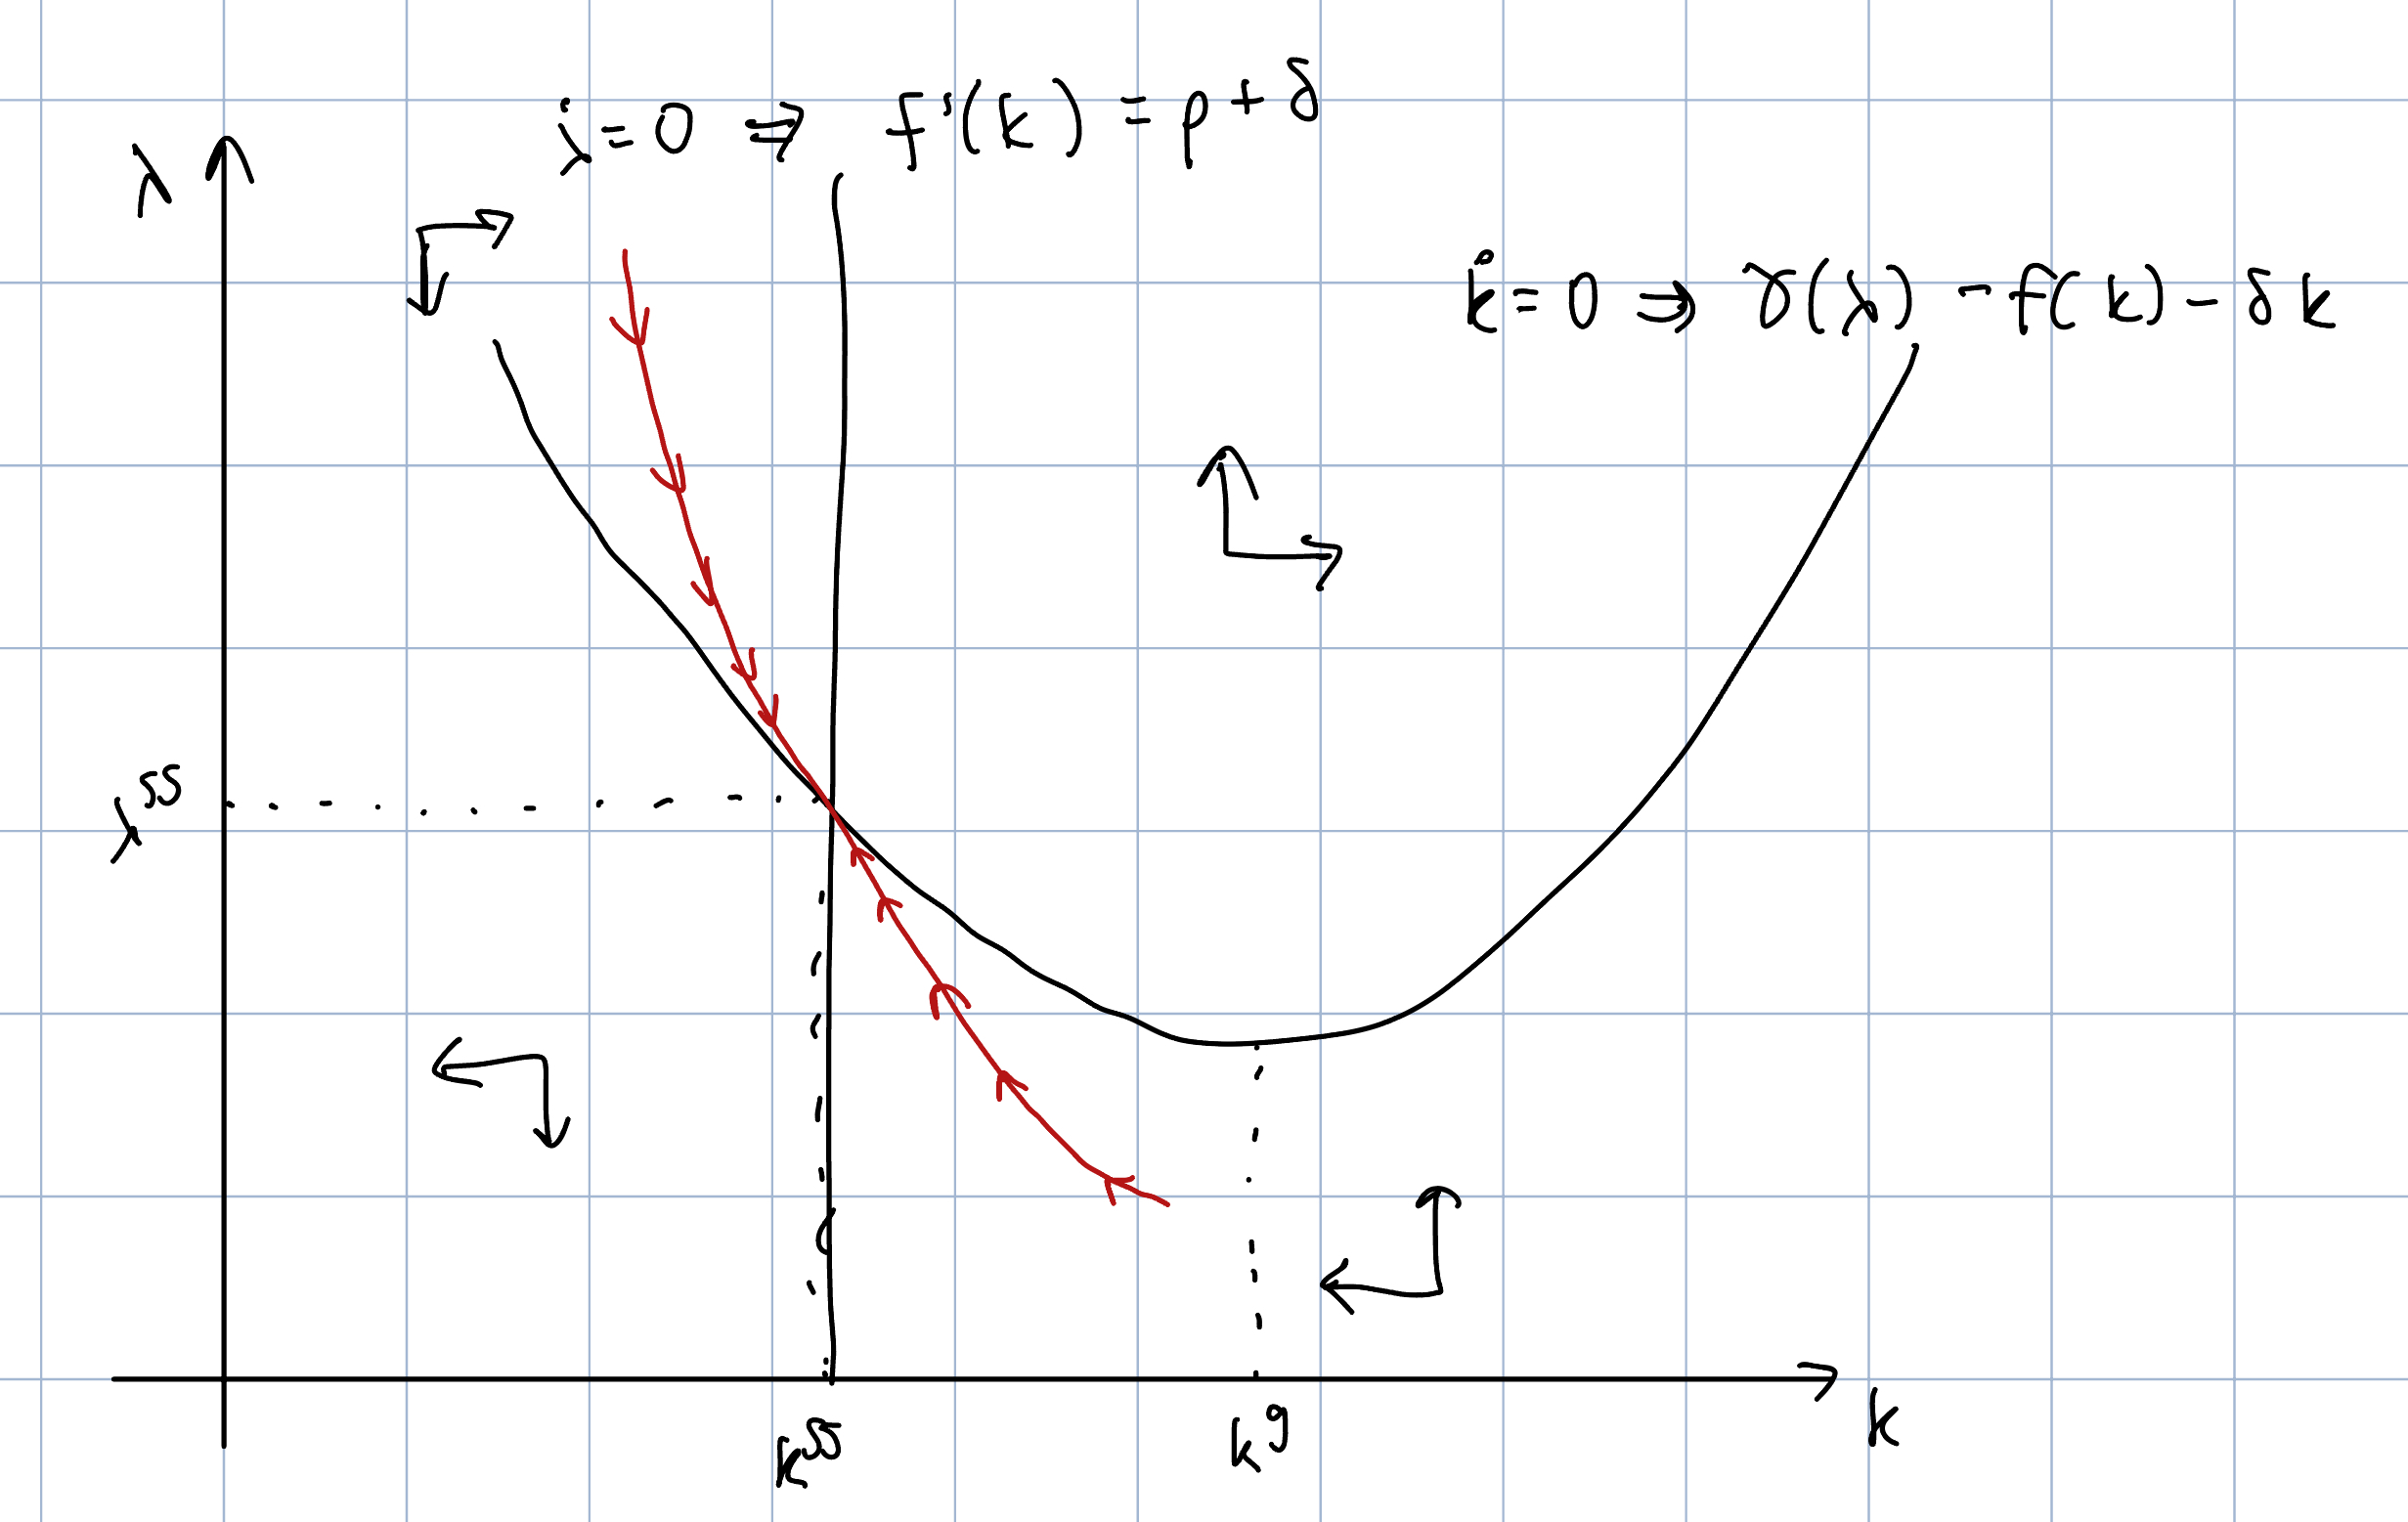
\includegraphics[width=0.9\textwidth]{10-14-1}
	\captionof{figure}{The Phase Diagram}
\end{center}

Put \[
	\mu(k) = u' \left[ f(k) - \delta k \right], \quad 0 < k \le \overline{k}
,\] 
where $\overline{k}$ is the largest maintainable capital stock, so $f(\overline{k}) = \delta \overline{k}$.

$\mu(k)$ is the marginal utility when $c = f(k) - \delta k$, so $(k,\mu(k))$ is the locus where $\dot{k} = 0$.

Differentiating, $\mu'(k) = u'' \left[ f(k)- \delta k \right] \left[ f'(k) - \delta \right].$ Since $u'' < 0$ and $f'(k^g) - \delta = 0$,
\begin{align*}
	\mu'(k) < 0, \quad \text{if } k < k^g \\
	\mu'(k) > 0, \quad \text{if } k > k^g
.\end{align*}

\subsection{Cass-Koopmans: Linear Approximation}
Linearize around the ODES (\ref{odelambda}, \ref{odek}) to get
\begin{align*}
	\dot{k}(t) &\approx \left( f' -\delta \right)(k-k^{ss}) - \gamma'(\lambda-\lambda^{ss}) \\
	\dot{\lambda}(t) &\approx -f''\lambda^{ss}(k-k^{s}) + \left( \delta + \rho - f' \right)(\lambda - ambda^{ss})
.\end{align*}
Substituting $f'(k^{ss}) = \rho + \delta$ and defining the deviations $x = k-k^{ss}, y = \lambda - \lambda^{ss}$, we get \[
	\begin{pmatrix}
	\dot{x} \\
	\dot{y}
	\end{pmatrix} \approx \begin{pmatrix}
	\rho & - \gamma'(\lambda^{ss}) \\
	-f''(k^{ss})\lambda^{ss} & 0
	\end{pmatrix} \begin{pmatrix}
	x  \\
	y
	\end{pmatrix} 
.\] 

Using the characteristic equation, we get the roots are of real and opposite sign. The particular solution of interest has the coefficient $0$ on the eigenvector associated with the positive eigenvalue, and the other coefficient is determined by the initial condition on the state variable. 

\section{Cass-Koopmans Model - Competitive Equilibrium Approach}
\subsection{Model Preliminaries}
Suppose all households are identical and identical firms have CRS technology. Add a government that taxes labor income at a flat rate and uses the revenue to finance lump-sum rebates. Households own the only asset, capital stock.

Let $w$ be the pre-tax wage, $R$ the rate of return on capital (rental price), $r$ the real interest rate, and $S$ the lump-sum rebate.

Assume $\rho > 0$ and $u(c,1-l)$ is strictly increasing, concave, strictly quasi-concave, and continuously differentiable with
\begin{align*}
	\lim\limits_{c \to 0} u_1(c,1-l) &= \infty, \quad \lim\limits_{l \to 1} u_2(c,1-l) = \infty, \\
	\lim\limits_{c \to \infty} u_1(c,1-l) &= 0, \quad \lim\limits_{l \to 0} u_2(c,1-l) = 0
.\end{align*}
Assume $\delta > 0$, $f(k,l)$ is strictly increasing, strictly quasi-concave, continuously differentiable with CRS, $f(0) = 0$, and Inada conditions for the limits as $k, l \to 0, \infty$.

\subsection{Optimization Problem of the Firm}
The representative firm takes as given prices $\{w(t), R(t), r(t)\}$. Their problem is\marginnote{The discounting rate of $-\int_{0}^{t} r(s)ds$ says that your profits at time $t$ are discounted by the interest rate, compounded over all time since the present. It replaces $rt$ as the interest rate can fluctuate over time.} \[
	\max_{\{k^d(t), l^d(t)\}} \int_{0}^{\infty} e^{-\int_{0}^{t} r(s)ds } \{f\left[ k^d(t), l^d(t) \right] - R(t) k^d(t) - w(t)l^d(t)\}dt 
.\] There is no intertemporal component. Profits must be zero because the firm has CRS --- it can shut down by demanding zero inputs and must have bounded profits.

Hence, in equilibrium, the solution must be interior and we have the FOCs
\begin{align*}
	f_k \left[ k^d(T), l^d(t) \right] &= R(t) \\
	f_l \left[ k^d(t), l^d(t) \right] &= w(t)
.\end{align*}
Because of CRS, only the ratio between $k^d$ and $l^d$ is pinned down from $(R,w)$.

\section{Wednesday, October 15: Nonlinear ODEs (TA Session \#3)}

The midterm will cover material until the end of week 3.

\subsection{Neoclassical Growth Model}
Recall that we have the two ODEs:
\begin{align*}
	\dot{\lambda}(t) &= \left( \rho + \delta - f'(k(t)) \right)\lambda(t) \\
	\dot{k}(t) &= f(k(t)) -\delta k(t) -\gamma(\lambda(t))
.\end{align*}

\begin{aside}
	If the problem is concave, then the transversality condition is also a sufficient condition. A steady state always solves the transversality conditions (assuming there is discounting).
\end{aside}
We take the two ODEs and use a first-order Taylor approximation around the steady state. Note that since the value we approximate around is the steady state where the rates of change are $0$, the only terms remaining are those attached to the deviation measures. 

Rewrite the deviations in the linearizations with $\dot{\lambda}^d, \dot{k}^d$
\begin{align*}
	\dot{\lambda}^d(t) &= -f''(k^{ss})\lambda^{ss} \cdot k^d(t) \\
	\dot{k}^d(t) &= -\gamma'(\lambda^{ss}) \cdot \lambda^d(t) + \rho \cdot k^d(t)
.\end{align*}
Then 
\[
	\begin{pmatrix}
	\dot{\lambda}^d(t)  \\
	\dot{k}^d(t)
	\end{pmatrix} = \begin{pmatrix}
	0 & -f''(k^{ss})\lambda^{ss} \\
	-\gamma'(\lambda^{ss}) & \rho
	\end{pmatrix} \begin{pmatrix}
	\lambda^d(t) \\
	k^d(t)
	\end{pmatrix} 
.\] 
The $2 \times 2$ matrix has $2$ eigenvectors: one positive and one negative. The positive eigenvector gets a constant of $0$ and the negative has its constant pinned down by the boundary conditions.

\subsection{Alternative: The Phase Diagram}
The $\dot{\lambda}$ locus is easy; it pins down a single value of $k$, called $k^{ss}$. The $\dot{k}$ locus is trickier; if we want to find where $k$ is increasing over time, we have that 
\begin{align*}
	0 &\le f(k(t)) - \delta k(t) - \gamma(\lambda(t)) \\
	\gamma(\lambda(t)) &\le f(k(t)) - \delta k(t) \\
		   \lambda(t) &\ge \gamma^{-1} \left[ f(k(t)) - \delta k(t) \right] 
.\end{align*}

Note that the inequality flips between the second and third lines because $\gamma^{-1}$ is a decreasing function. So $k$ increases when $\lambda$ is high.

Since $f(k)-\delta(k)$ is concave and $\gamma^{-1}$ is downward sloping (since $u'$ is downward sloping), the $\dot{k} = 0$ locus is convex. Its minimum is to the right of $k^{ss}$ for reasons explained in class.


\section{Thursday, October 16: NCG, Cont'd. and Sustained Long-Run Growth}
\subsection{Optimization of the Household}
The household solves 
\begin{align*}
	\max_{\{c(t), l^s(t), k^s(t)\}} &\int_{0}^{\infty} e^{-\rho t}u\left[ c(t), 1- l^s(t) \right] dt \\
	\text{s.t. } k^s(t) &= [R(t)-\delta]k^s(t) + (1-\tau)w(t) l^s(t) + S(t) - c(t) \\
	\lim\limits_{t \to \infty} k^s(t) &\ge 0 \\
	k^s(0) &= k_0 > 0
.\end{align*}

Putting $H_c = 0, H_l =0, \rho \lambda-H_k = \dot{\lambda}, H_\lambda = \dot{k}^s$, we have two controls, one state, and one costate. The problem is simpler when we eliminate the controls and solve it interms of the state and costate.

\subsection{Equilibrium and Characterizing the Solution}
We have the household budget constraint from the problem and the government's constraint is $S(t) = \tau w(t)l^s(t)$. Imposing market clearing on capital, labor, and the goods market ($f(k(t),l(t)) = c(t) + \delta k(t) + \dot{k}(t)$), we can get that \[
	f(k(t),l(t)) = R(t)k(t) + w(t)l(t) 
.\] We didn't need the condition of the goods market clearing because of Walras' Law\footnote{Actually Euler's theorem for homogeneous functions}, which automatically tells us \[
	f(k(t),l(t)) = f_k(k(t),l(t))k(t) + f_l(k(t),l(t))l(t)
.\] 

If we use the FOCs to write prices in terms of quantities, we can characterize the solution through quantities, as we have previously eliminated controls. Once finding states and costates, we can back out the controls and prices.

By imposing functional forms, we can get laws of motion: explicit expressions for $\frac{\dot{\lambda}}{\lambda}$ and $\dot{k}$. These pin down loci, where $\dot{\lambda} = 0$ leads to a ray from the origin and $\dot{k} = 0$ leads to a curve. If they intersect once, there is a unique steady state. 

Differentiating the expression for $l$ with respect to $\tau$, we see that a lax on labor income shifts households from consumption to untaxed leisure. The reduction in labor supply leads to a decrease in the marginal product of capital, which decreases the steady state capital stock. 

\subsection{Sustained Long-Run Growth: Labor-Augmenting Technical Change}

In the previous model, there was no sustained growth in consumption per capita.\marginnote{The problem was that the production function was CRS in (labor $\times $ capital) and hence DRS in capital, since labor was constant. This motivates adding technology growth to increase effective labor.} We first induce this growth by adding exogenous labor-augmenting technological change. In this model (and the others to follow), we want to have a balanced growth path.

\begin{defn}[Balanced growth path]
	On a BGP, the consumer is optimizing and choosing a constant rate of consumption growth, supplies a constant amount of labor, and has a wage that grows at the rate of consumption.
\end{defn}

Economists have backed out what functional forms on preferences are needed for a BGP.

Suppose technology improves at the constant rate $g > 0$. Using capital letters to denote aggregate quantities,
\begin{align*}
	Y(t) &= F(K(t),L(t),t) = F(K(t),e^{gt}L(t)) , \\
	\text{and assume CIES } u(\hat{c}) &= \begin{cases}
		\frac{\hat{c}^{1-\theta}}{1-\theta}, \quad \theta \in (0,1) \\
		\ln{(\hat{c})} = \lim\limits_{\theta \to 1} \frac{\hat{c}^{1-\theta} - 1}{1-\theta} 
	\end{cases}.
\end{align*}

Assuming constant rate of population growth at $n$ from the initial population $N_0$, the dynasty's problem is
\begin{align*}
	\max_{\{\hat{c}(t)\}} &\int_{0}^{\infty} e^{-\rho t} N_0 e^{nt} \frac{\hat{c}(t)^{1-\theta}}{1-\theta} dt \\
		\text{s.t. } C(t) &= N_0 e^{nt} \hat{c}(t) \\
		\dot{K}(t) &= F\left( K(t), N_0 e^{\left( n+g \right)t} \right) - \delta K(t) - C(t) \\
		0 &\le C(t) \le F\left( K(t), N_0 e^{\left( n+g \right)t}\right) \\
		K(0) &= K_0 > 0
.\end{align*}

We want to rewrite and solve the problem from a per effective labor perspective, not in the aggregate. Define $c(t), k(t)$ as consumption and capital \emph{per unit of effective labor}\marginnote{Note that the exponents are different because $\hat{c}$ is consumption \emph{per person}, while $K$ is the totla capital stock.}: \[
	c(t) = e^{-gt} \hat{c}(t), \quad k(t) = \frac{1}{N_0} e^{-\left( n+g \right)t K(t)}
.\] 

Rewriting the problem in terms of units per effective labor, the problem becomes \[
	N_0 \max_{\{c(t)\}} \int_{0}^{\infty} e^{-\hat{\rho}t} \frac{c(t)^{1-\theta}}{1-\theta}dt 
,\] where $\hat{\rho} = \rho - n - \left( 1-\theta \right)g$. The restriction $\hat{\rho} > 0$ requires $\rho > n + \left( 1-\theta \right)g$; otherwise, the objective function is unbounded above.

To get a LOM for $k$ using the LOM for $\dot{K}$ that we already have, write \[
	k(t) = \frac{1}{N_0} e^{-\left( n+g \right)t}K(t)
\] and differentiate. Then \[
	\dot{k}(t) = f(k(t)) - \hat{\delta} k(t) - c(t)
,\] where $\hat{\delta} = \delta + n + g$.

\subsection{Growth with Endogenous Labor Supply}

Now suppose that in addition to exogenous technical change, there is endogenous labor supply. On a BGP, per capital consumption $\hat{c}$ is growing but labor and leisure per capita are constant. 

The required preferences are \[
	u(\hat{c},l) = \begin{cases}
		\frac{1}{1-\theta} \left( \hat{c}v(l) \right)^{1-\theta}, \quad \theta \in (0,1) \\
		u(\hat{c},l) = \ln{(\hat{c})} + v\left( l \right), \quad \theta = 1
	\end{cases}
,\] where $v$ is increasing and concave and $u$ is concave. Note that the MRS between leisure and consumption grows at the same rate as consumption for constant $l$: \[
	\frac{u_l(\hat{c},l)}{u_c(\hat{c},l)} = \frac{\hat{c}v'(l)}{v(l)}
.\] 
If the wage rate grows at the same rate as per capita consumption, then constant labor supply is an optimal choice.

\subsection{Growth with Investment-Specific Technical Change}

Now suppose the price of investment goods, new capital goods, declines relative to the price of consumption goods. We will have two kinds of capital: equipment (falling price) and structures (constant price). See Greenwood, Hercowitz, and Krusell (1997) for more.

Let the price of equipment be $q(t) = e^{-\eta t}q_0$.

In a BGP, the technology must be Cobb-Douglas. GHK find that 60\% of growth comes from ISTC and 40\% from labor-augmenting TC.

\subsection{Endogenous Growth}

In the Cass-Koopmans model, $L$ was fixed and $F$ had DRS in the producible factor $K$. 

Rebelo puts $Y = AK$ for $K$ including both human and physical capital, so the problem is
\begin{align*}
	\max \int_{0}^{\infty} & e^{-\rho t} \frac{c(t)^{1-\sigma}}{1-\sigma}dt \\
	\text{s.t. } \dot{k}(t) &= Ak(t) - c(t)
,\end{align*} where $A > \rho$.

Then
\begin{align*}
	H(k,c,\lambda) &= \frac{c(t)^{1-\sigma}}{1-\sigma} + \lambda \left( Ak - c \right) \\
	\implies \frac{\dot{c}}{c} &= -\frac{1}{\sigma} \frac{\dot{\lambda}}{\lambda} = \frac{A-\rho}{\sigma} =: g
.\end{align*}
Since consumption growth is constant, capital must grow at a constant rate too, so $\frac{c}{k} = \gamma$ is also constant. The same portion of output is consumed over time.

\section{Tuesday, October 21: Deterministic Dynamic Programming}
\subsection{Overview}
We will mostly consider dynamic programming in a discrete, infinite-horizon context. Some advantages of dynamic programming over optimal control include ease of adding exogenous shocks and matching data.

We have the Social Planner's problem
\begin{align*}
	v(k_0) &= max_{\{c_t, k_{t+1}\}} \left[ u(c_0) + \underbrace{\sum\limits_{t=1}^{\infty} \beta^{t}u(c_t)}_{\beta v(k_1) = \beta \sum\limits_{t=0}^{\infty} \beta^{t}u(c_{t+1})} \right] \\
	c_t + k_{t+1} &\le f(k_t) + (1-\delta)k_t, \\
	c_t &\ge 0, \quad k_{t+1} \ge 0
.\end{align*}
Note that $\beta$ is now the discount factor and can be put as $\frac{1}{1+\rho}$. 

The Principle of Optimality says that if a candidate solution $\{c_t, k_{t+1}\}$ is optimal from $t=0$, the continuation is optimal from $t=1$ on. This is satisfied because the objective function is additively separable over time with a constant discount factor.

Hence we can rewrite the problem as
\begin{align*}
	\hat{v}(k) &= \max_{c\ge 0,y \ge 0} \left[ u(c) + \beta\hat{v}(y) \right]  \\
	\text{s.t.} \quad c+ y &\le f(k) + (1-\delta)k
.\end{align*}
The problem appears simpler, but we don't know what $\hat{v}$ is. We wonder:
\begin{itemize}
	\item Does $\hat{v}$ agree with $v(\cdot)$ as an infinite sum?
	\item Is $v$ the unique solution to this recursive problem?
	\item What are the properties of the optimal $c$ and $y$?
	\item How can we get a numerical approximation to the solution?
\end{itemize}

The \emph{primitives} for the Planner's problem are the objective function, discount factor, and the constraints. 

\subsection{Dynamic Programming in the Cass-Koopmans Model}
Consider a discrete version of the Cass-Koopmans model with no population growth, no technical change, and no taxes.
The value function is defined by
\begin{equation}
	v(k_0) = \sup\limits_{\{k_{t+1}\}} \sum\limits_{t=0}^{\infty} \beta^t u\left( f(k+1) + (1-\delta)k_t - k_{t+1} \right) \label{eq:10-21-SP}
\end{equation}
such that $k_{t+1} \in \left[ 0, f(k_t) + (1-\delta)k_t \right] =: [m(k),M(k)]$.

Use the state space of $K = [0,\overline{k}]$, where $\overline{k} = k^g$ is defined by $f'(k^g) = \delta$. The Bellman is
\begin{equation}
	\hat{v}(k) = \max_{y \in [0,f(k) + (1-\delta)k]} u\left( f(k) + (1-\delta)k - y \right) + \beta \hat{v}(y) \label{eq:10-21-BE}
,\end{equation}
where $y$ is the capital carried over to the next period.
The current period return function is
\begin{equation}
	F(k,y) = u\left( f(k) + (1-\delta)k - y \right) \label{eq:10-21-F}
.\end{equation}

We have the following assumptions:
\begin{itemize}
	\item $\beta \in (0,1)$
	\item $u$ and $f$ are strictly increasing, strictly concave, $C^2$, and satisfy Inada conditions with $u(0) = 0$, $f(0) = 0$.
\end{itemize}

Note that the functions $m,M$ for the boundaries on the choice set are continuous and bounded for each $k$. Furthermore, the current period return is continuous and bounded on the set $A$ where \[
	A = \{(k,y) : k \in K, y \in [0,M(k)]\}
.\] 

$A$ is the feasible set for $(k,y)$. Since $M(k)$ is concave and $m(k) = 0$, the graph of $A$ is a convex set.
\begin{center}
	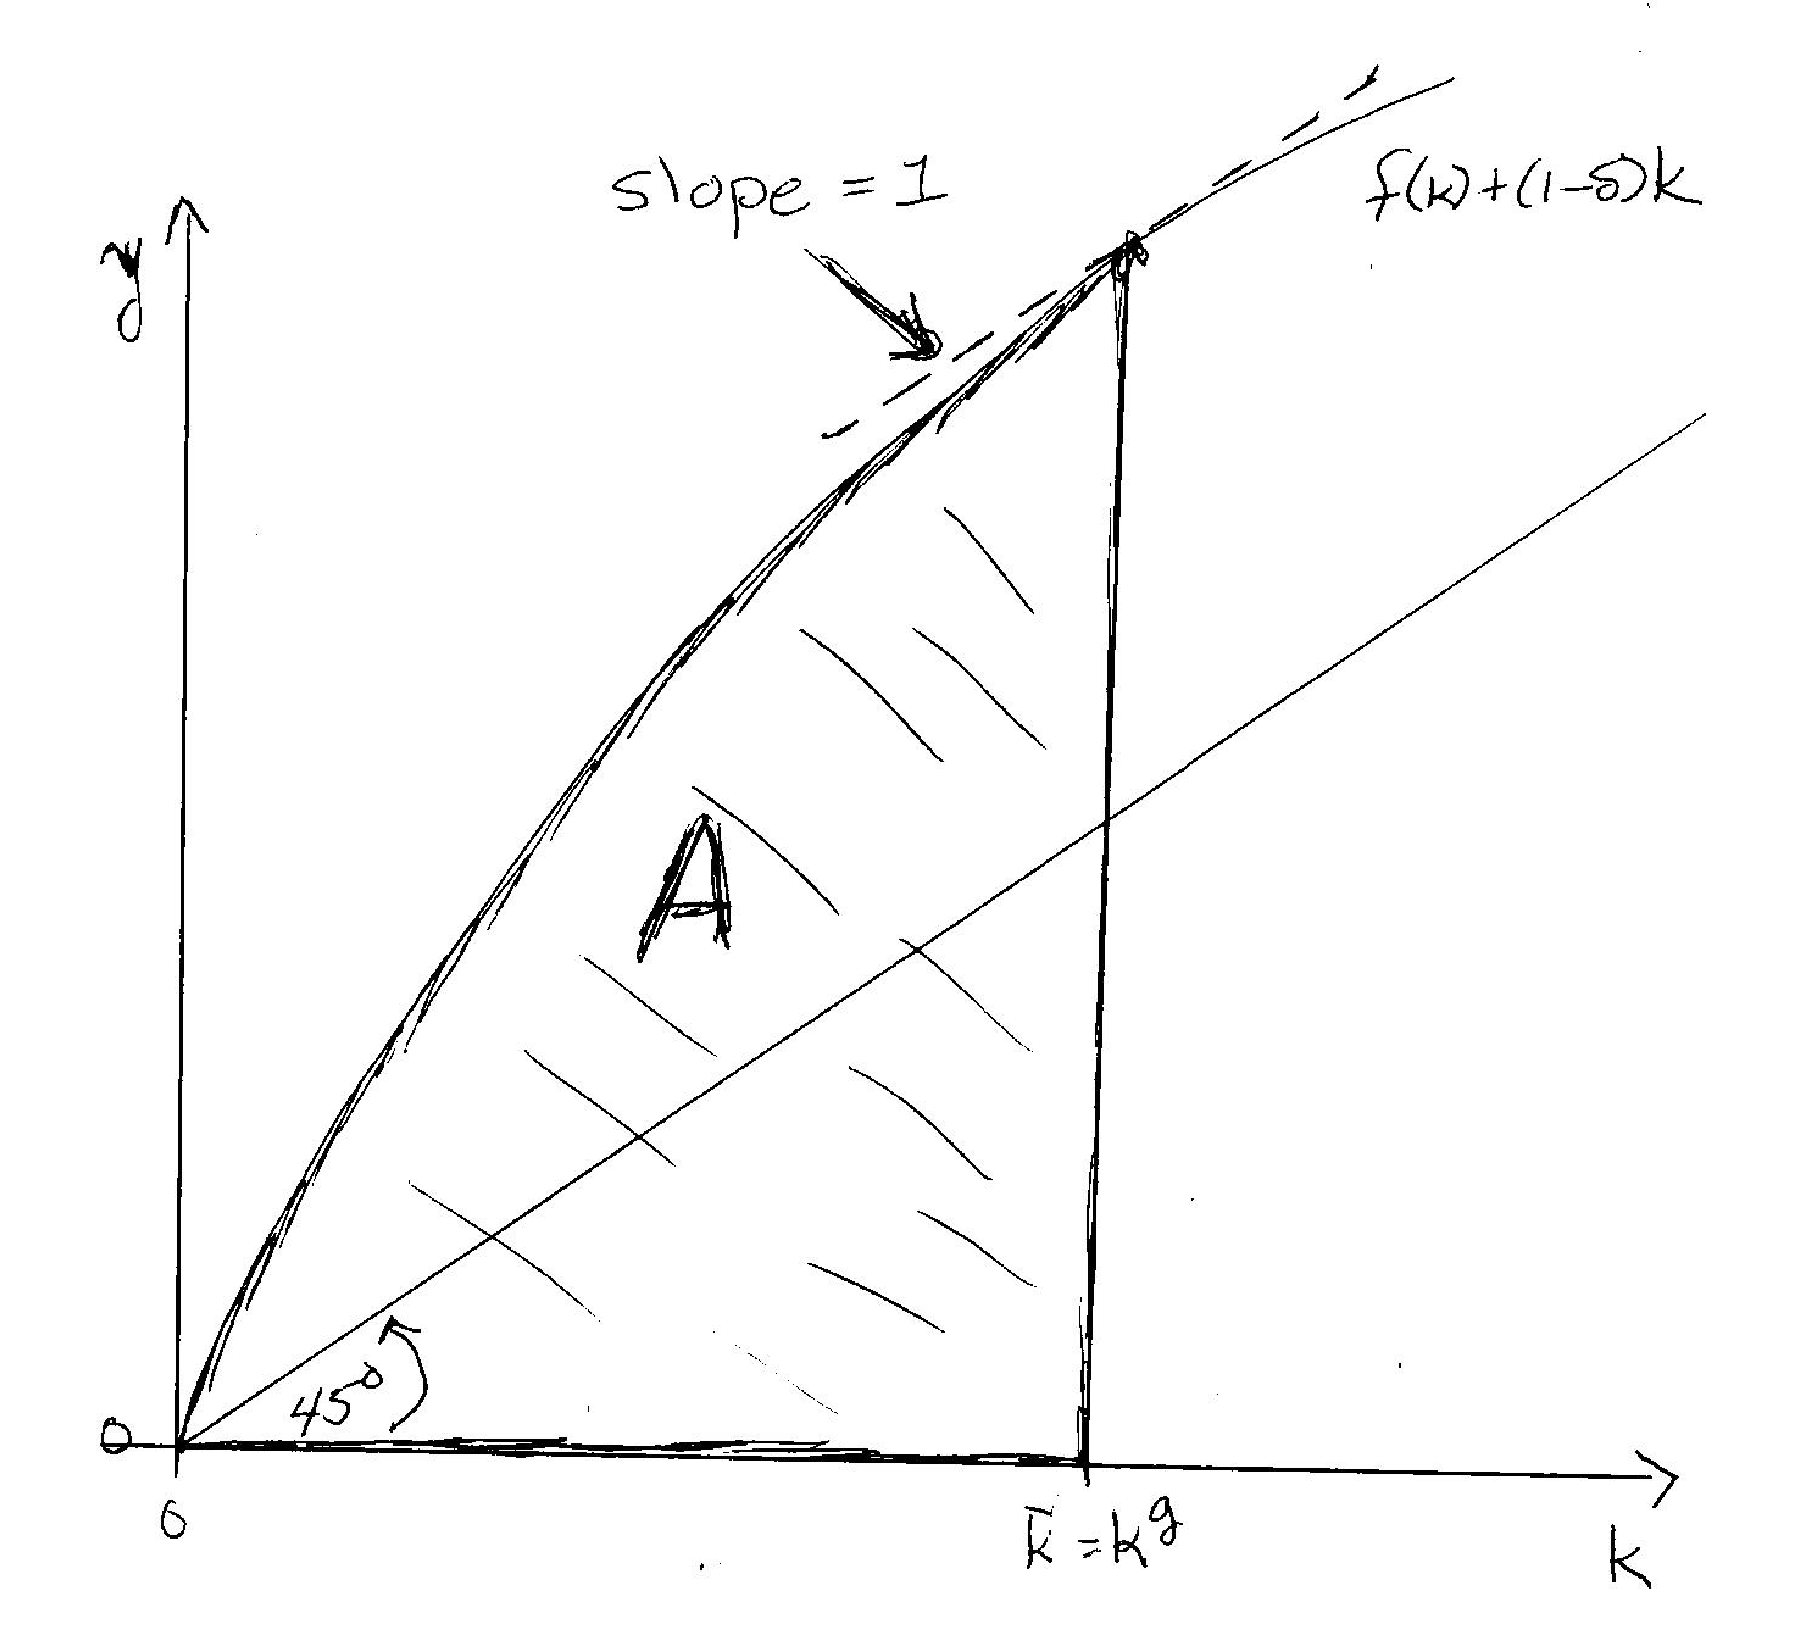
\includegraphics[width=0.7\textwidth]{10-21-1}
	\captionof{figure}{Convexity of $A$}
\end{center}
Furthermore, $F(k,y)$ is concave in $(k,y)$ and strictly concave in $k$. Putting $g(k) = k'$ as the unique optimal choice for the capital stock next period, the optimal consumption is \[
	c(k) = f(k) + (1-\delta)k - g(k)
.\] 

Inada conditions on $u$ and $f$ guaranteed that for $k > 0$, the optimal choice of $y$ is not at the boundary of the feasible set. Using the Bellman (\ref{eq:10-21-BE}), we get the FOC \[
	u'\left( F(k) + (1-\delta)k - g_(k) \right) = \beta v'(g(k))
.\] The LHS is increasing in $y$ and the RHS is decreasing in $y$. Examining behavior as $y\to 0$ and $y\to f(k) + (1-\delta)k$, we see that there is a unique solution (and so it must be $y = g(k)$ by definition.

The envelope condition on the Bellman says \[
	v'(k) = \left( f'(k) + (1-\delta)k \right) u'\left( f(k) + (1-\delta)k - y \right)
.\] Plugging in $g(k)$ for $y$ in the FOC and replacing $v'(g(k))$ with the envelope condition, 
\begin{align*}
	0 &= -u'\left( f(k) + (1-\delta)k - g(k) \right) + \beta \left( f'(g\left( k \right) + (1-\delta)\right) u'\left( f(g(k)) + (1-\delta)g(k) - g(g(k)) \right) \\ 
	\implies 1 &= \beta \left( f'(k^{ss}) + (1-\delta) \right) \text{ because } g(k^{ss}) = k^{ss}\\
	\frac{1}{\beta} &= f'(k^{ss}) + 1 - \delta \\
	f'(k^{ss}) &= \rho + \delta
.\end{align*}

To examine transitional dynamics, we see that $u,f \in C^2 \implies F \in C^2$, so we can write the linearized Euler Equation: \[
	0 = F_{12}z_t + F_{22}z_{t+1} + \beta\left[ F_{11} z_{t+1} + F_{12} z_{t+2} \right] 
.\] \marginnote{The Euler equation contains first derivatives and we linearize with deviations $z_t, z_{t+1}$ in $k, k_{t+1}$. }
The second-order ODE can be written \[
	\begin{pmatrix}
	z_{t+2} \\
	z_{t+1}
	\end{pmatrix} = \begin{pmatrix}
	J & K \\
	1 & 0
	\end{pmatrix} \begin{pmatrix}
	z_{t+1} \\
	z_t
	\end{pmatrix} 
,\] where $J$ and $K$ are in terms of $u''$ and $f''(k)$.

\subsection{Deterministic Dynamic Programming: The Canonical Model}

We generalize the dynamic programming method.

Given the primitives:
\begin{itemize}
	\item A return function $F(x,y)$ 
	\item The discount factor $\beta \in (0,1)$ 
	\item Feasibility constraints $y \in \left[ m(x),M(x) \right] $,
\end{itemize}

We can write the sequence problem by defining
\begin{align*}
	v(x_0) &= \sup\limits_{\{x_{t+1}\}} \sum\limits_{t=0}^{\infty} \beta^t F(x_t,x_{t+1}) \\
	\text{s.t. } x_{t+1} &\in \left[ m(x), M(x) \right] 
\end{align*}
then choosing a state space $X$ and writing the Bellman \[
	\hat{v}(x) = \max_{y \in [m(x), M(x)]} F(x,y) + \beta \hat{v}(y)
.\] 
This is a functional equation in the unknown function $\hat{v}$. The value function is as defined with $v$, and we are interested in if $v$ solves the equation with $\hat{v}$. 

If the following basic assumptions hold --- 
\begin{itemize}
	\item The feasible set $[m(x),M(x)]$ is bounded for each $x \in X$, and $m,M$ are continuous,
	\item The return $F(x,y)$ is bounded and continuous, and
	\item $\beta \in (0,1)$
\end{itemize}
--- then 
\begin{itemize}
	\item We can use the Contraction Mapping Theorem on the operator $T$ defined by \[
		T \phi(x) = \max_{y \in \left[ m(x),M(x) \right]} F(x,y) + \beta \phi(y)
	\] to see there is a unique, bounded, continuous function $v$ satisfying the Bellman
	\item This function is the one defined in the Social Planner's problem
	\item The set of maximizing values for $y$ (called $G(x)$) is nonempty and upper-hemicontinuous
	\item Starting from $v_0$ as a bounded, continuous function, $v$ can be computed by successive approximations where $v_{n+1} = Tv$ satisfies $v_n \to v$ at a rate of convergence of $\beta$.
\end{itemize}

\section{Stochastic Dynamic Programming}
\subsection{Lucas and Prescott: Setup}
We first look at Lucas and Prescott's model of industry investment under uncertainty. 
Consider a perfectly competitive industry where:
\begin{enumerate}[(i)]
	\item All firms have the same CRS technology with capital as the only input, $Q_i = X_i$
	\item The cost of investment depends on current capital: \[
		C(X_i;,X_i) = X_i c(X_i',x_i)
	,\] wheere \[
		c(1-\delta)=0
	\] and $\cdot$ is strictly increasing and strictly convex
	\item Industry demand is stochastic with demand shock $z \in Z$. $D(\cdot, z)$ is a downward sloping demand curve and $U$ is the area under it\marginnote{$U$ is strictly increasing and strictly concave in $q$. We also assume that it is uniformly bounded}: \[
		U(q,z) = \int_{0}^{q} D(v,z)dv 
	.\] 
	\item Put $x = \sum_i X_i$ has industry capital stock so total output is \[
		q= \sum Q_i = \sum X_i = x
	.\] 
\end{enumerate}

We suppose the Invisible Hand solves \[
	v(x_0,z_0) = \sup \E_0\left[\sum\limits_{t=0}^{\infty} \left( \frac{1}{1+r} \right)^t \left[ U(x_t,z_t) - x_t c(\frac{x_{t+1}}{x_t}) \right] \mid z_0\right] 
\] given $x_0 > 0$, where the expectation is taken over future shocks conditional on the initial shock $z_0$.

The economy has two state variables: the endogenous capital stock $x$ and the current value $z$ for the exogenous demand shock. We choose our state space as follows:
\begin{itemize}
	\item For $x$, let $X = [\epsilon,M]$ for $\epsilon$ small and $M$ large.
	\item Assume $z \in Z = \left[ \underline{z}, \overline{z} \right]$ and there is a transition function $q(z,z')$ on $Z$ where $q(z, \cdot)$ is the density of $z'$ next period.
\end{itemize}
We then define the value function $v: X\times Z \to \R$.

The return function is \[
	F(x,y,z) = U(x,z) - xc(\frac{y}{x})
\] and the feasible set of choice of $y$, next period's capital, is \[
	\Gamma(x,z) = \left[ (1-\delta)x, M \right] 
.\] 

\subsection{Defining the Shock Process}
We need the following assumptions so our results from deterministic dynamic programming carry over:
\begin{enumerate}[(i)]
	\item The shocks follow a first-order Markov process with stationary transition function\marginnote{A finite $n$th-order Markov process can be written as a first-order process by expanding the state space to be of tuples length $n$.}
	\item Either:
		\begin{itemize}
			\item $Z = \{z_1,z_2,\ldots\}$ is a countable set and $Q = \left[ q_{ij} \right] $ is a transition matrix
			\item $Z \subseteq \R^k$ is a closed rectangle and for each $z \in Z$, there is a continuous density $q(z,\cdot)$ describing next period's shock distribution. Assume $q$ is continuous in its first argument ensuring that $Q$ has the \emph{Feller property}.\marginnote{The Feller property says if $h(z)$ is continuous in $z$, the function \[
						(Mh)(z) = \E\left[h(z') \mid z\right] = \int_{}^{} h(z')q(z,z')dz' 
			\] is continuous in $z$, where $M$ is an operator on the function $h$. In other words, a small perturbation in today's shcok does not change tomorrow's shock value very much.}
		\end{itemize}
\end{enumerate}
We say the transition function $Q$ is monotone if for any nondecreasing function $h$, $Mh$ is also nondecreasing.

\subsection{Solving the Model}
The Bellman equation is \[
	v(x,z) = \max_{y \in \left[ (1-\delta)x,M \right] } \left[ U(x,z) - xc(\frac{y}{x}) + \frac{1}{1+r} \int_{}^{} v(y,z')q(z,z') dz'  \right] 
.\] Under some assumptions, there exists a unique bounded continuous function $v$ that solves the Bellman equation by way of the Contraction Mapping Theorem. The optimal policy function $g(x,z)$ is single-valued, continuous, and strictly increasing in $x$. 

\marginnote{
\begin{center}
	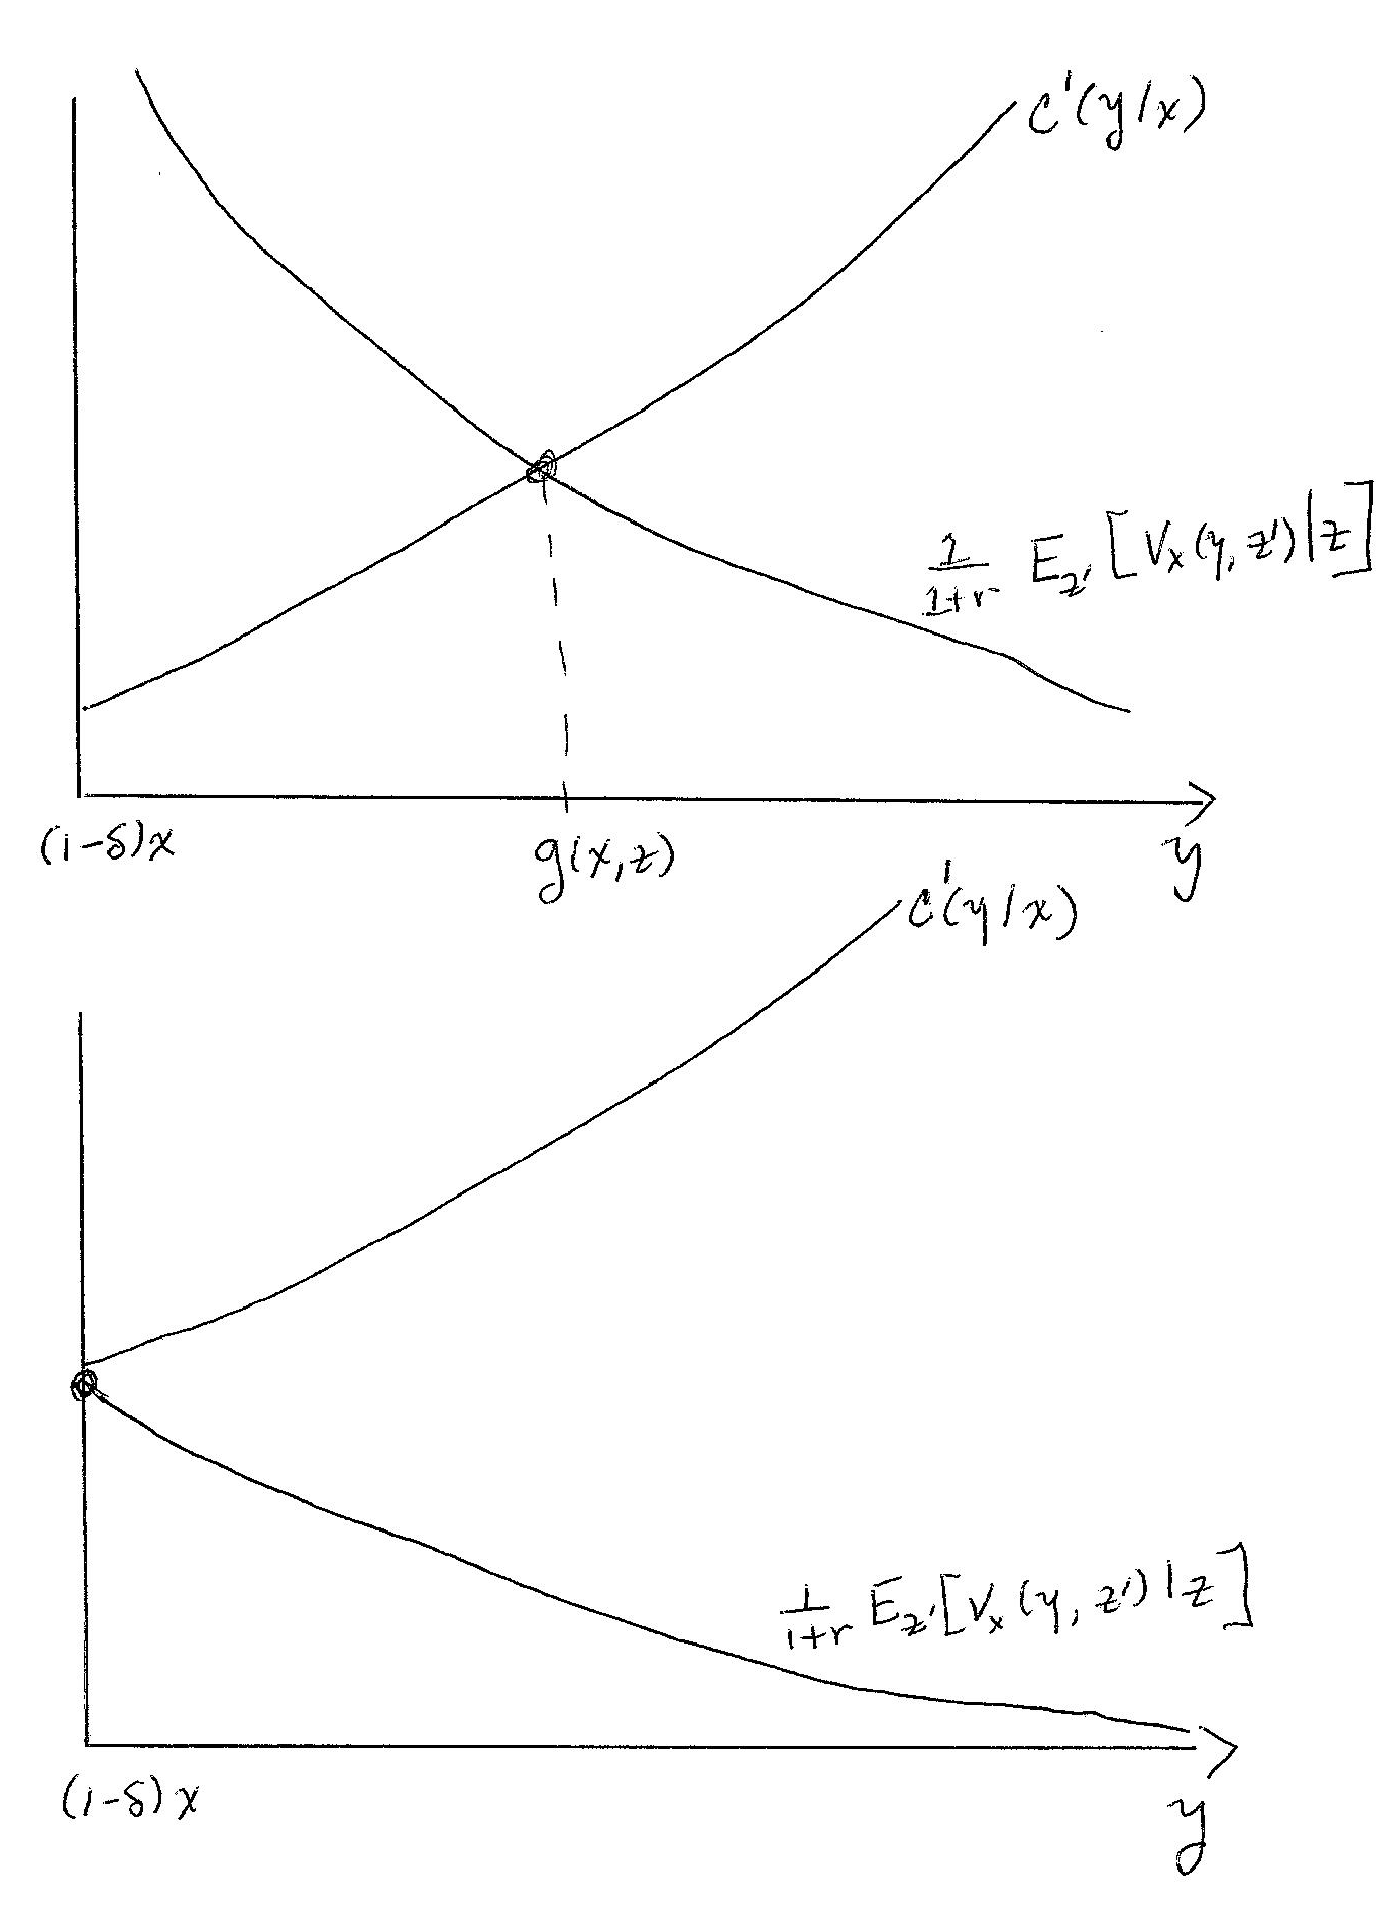
\includegraphics[width=0.5\textwidth]{11-4-1}
	\captionof{figure}{Interior solution and corner solutions to the planner's problem.}
\end{center}}
The FOC is \[
	c'(\frac{y^*}{x}) \ge \frac{1}{1+r} \int_{}^{} v_x(y^*,z')q(z,z')dz' 
\] with equality if \[
	y^* = g(x,z) > (1-\delta)x
.\] the LHS is increasing in $y$ and the RHS decreasing in $y$.

How do the two curves shift as $x$ and $z$ change? An increase in $x$ shifts the left boundary rightward, has no effect on the RHS, and shifts the LHS rightward. So if the solution is interior, it increases, but by less than the factor that $x$ increased by. If it is at the boundary, it increases by the same factor as $x$. So $g$ is strictly increasing in $x$ with a slope that is $1$ at a corner solution and less than $1$ at an interior solution.

An increase in $z$ does not affect the LHS, but we are not sure how it changes the RHS.\marginnote{\texthl{review why!}}

\subsection{Canonical Stochastic Dynamic Programming Model}

\begin{thm}
	If $h: X \times Z \to \R$ is bounded and continuous and $Q$ has the Feller property, then \[
		(Mh)(y,z) = \int_{-\infty}^{\infty}h(y,z')q(z,z')dz' 
	\] is also bounded and continuous. Furthermore, $Mh$ inherits (strict) monotonicity and (strict) concavity from $h$ in $y$.
\end{thm}

With this, we can apply arguments from the deterministic case. Define the operator $T$ on $C(S)$ by 
\begin{align*}
	Tf(x,z) &= \sup_{y \in \Gamma(x,z)} \left\{ F(x,y,z) + \beta \int_{} f(y,z')q(z,z')dz'  \right\} \\
			&= \sup_{y \in \Gamma(x,z)} \left[ F(x,y,z) + \beta \left( Mf \right)(y,z) \right] 
.\end{align*}

Obviously a stochastic system cannot have a steady state, since the shock is changing every period. The policy function $g$ and the transition function $Q$ for the shocks define a transition function $P$ on the state space $S = X\times Z$. If $Q$ has the Feller property and $g$ is continuous, then $P$ has the Feller property. 

The probability measure for the state next period is calculated by using the policy function $g(x,z)$ and the transition function $Q$ state-by-state, weighting with the probability measure $\lambda$. A new probability measure is produced, which we call \marginnote{
\begin{center}
	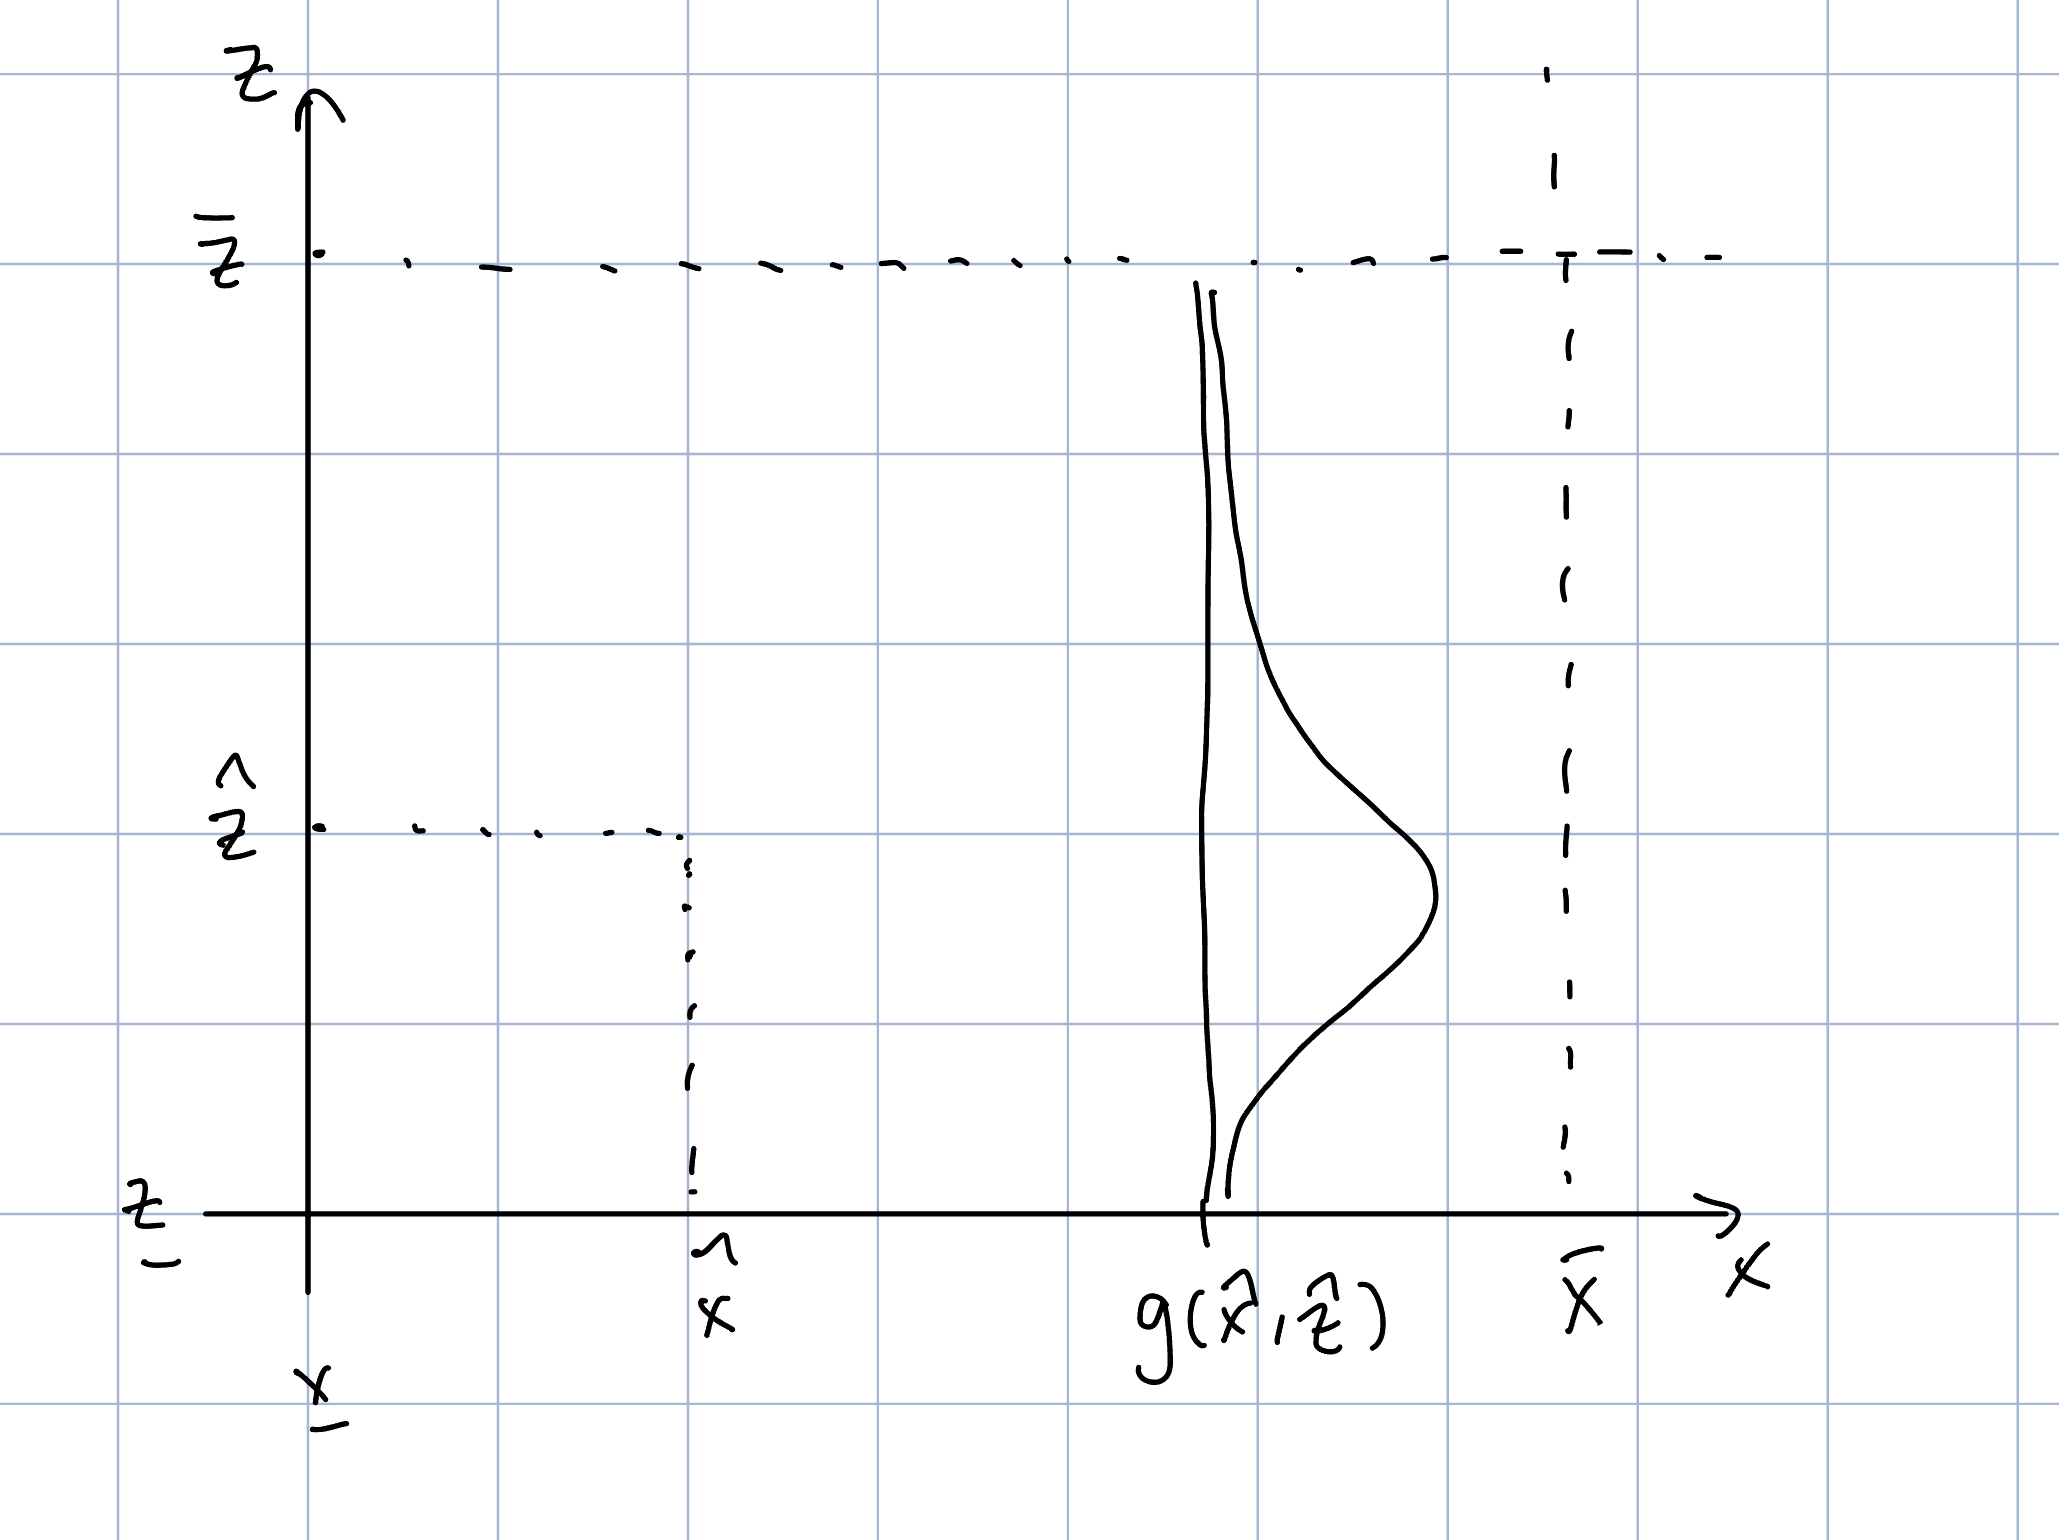
\includegraphics[width=0.5\textwidth]{11-6-1}
	\captionof{figure}{A new probability measure}
\end{center}
}\[
	 \lambda' = T^*\lambda
 ,\] where $T^*$ is the operator on measures associated with $P$. An invariant distribution will be a fixed point of $T^*$.

\section{Commodity Prices - Deaton and Laroque (1992)}
\subsection{Background on the Paper}
Prices for agricultural commodities fluctuate wildly from year to year. There are "greedy" speculators that hold inventory to take advantage of the price swings. Economists wondered if they stabilize or destabilize prices. \marginnote{
\begin{center}
	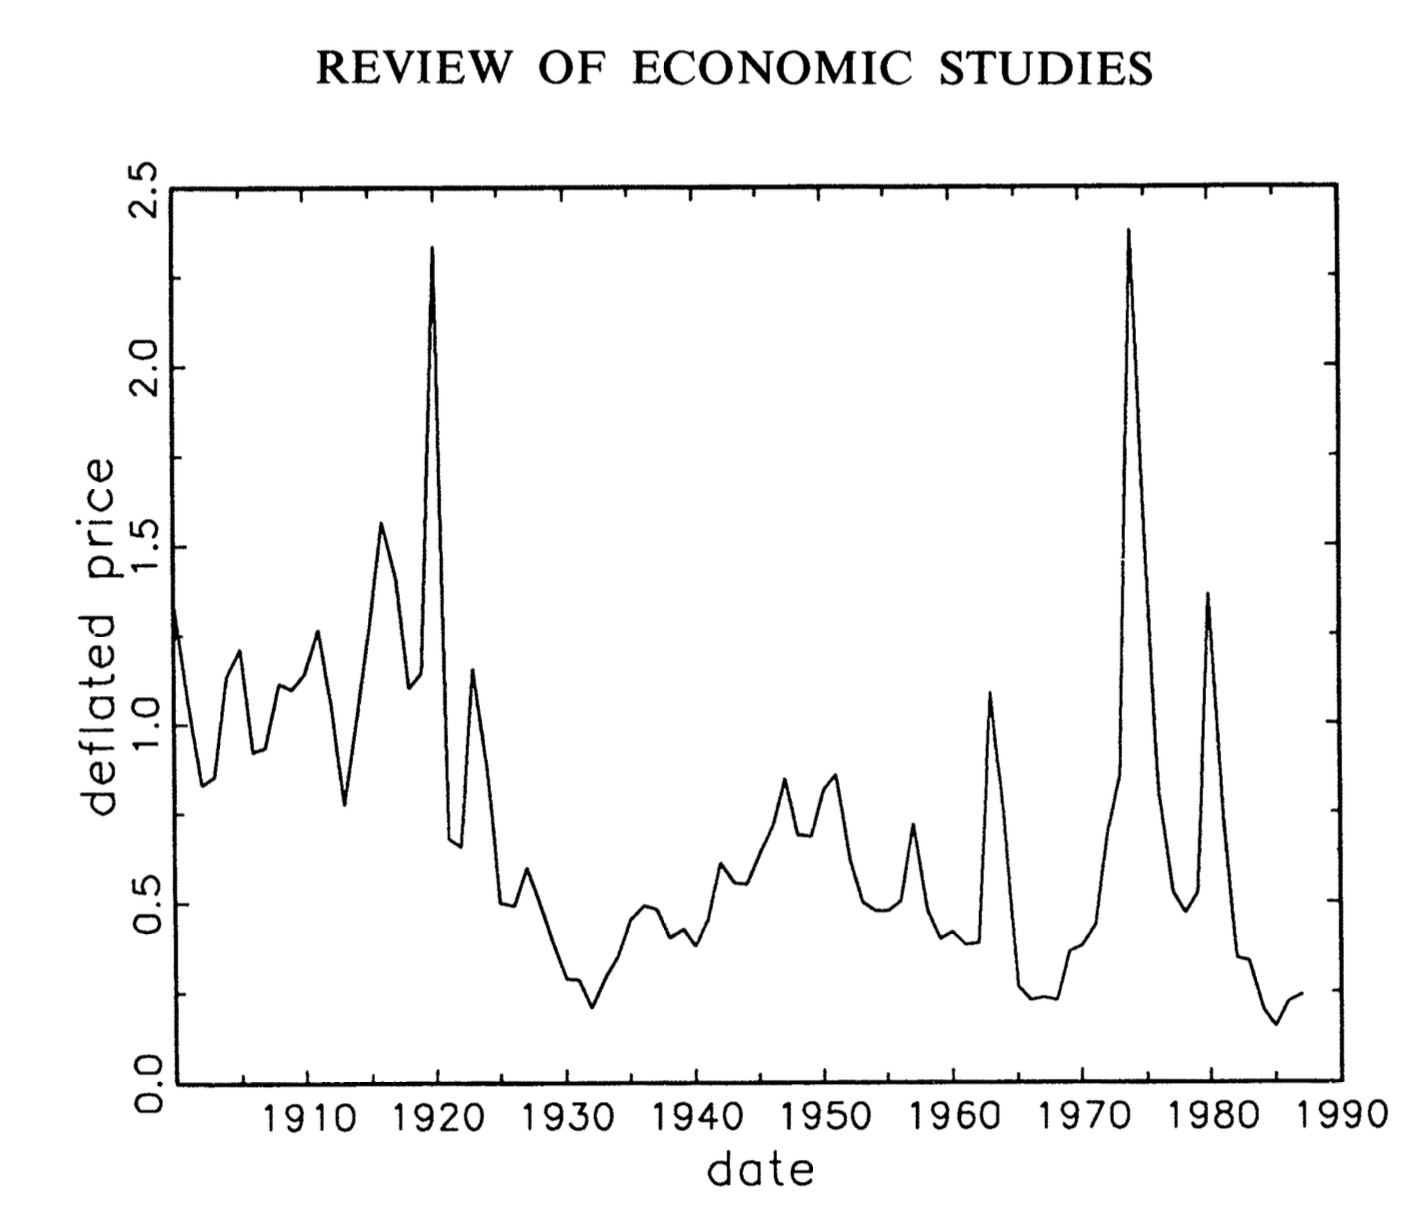
\includegraphics[width=0.5\textwidth]{11-6-2}
	\captionof{figure}{Sugar prices from Deaton and Laroque (1992)}
\end{center}}Looking at the price of sugar over time, price swings are asymmetric, with only upward spikes. Furthermore, the authors found that prices display high serial correlation. In this model, production is stochastic and goods can be stored.

\subsection{Model Overview}
The market is perfectly competitive, buyers are represented by a stationary and deterministic demand curve $D(q)$. On the sellers' side, each period endows the sellers with a random endowment (their aggregate output) $\omega_t$, which is i.i.d. year-to-year on the interval $[m,M]$. Let $\mu(\omega)$ be the density function for $\omega$. The speculators (just considered to be the producers themselves) can store $y$ units for one period with cost $\phi(y)$, where $\phi$ is strictly increasing, strictly convex, $C^1$ and $\phi(0) = 0$.\marginnote{Another way to make storage costly is to assume inventories depreciate.} Each period, the producers decide how much to sell and how much to carry forward as inventories.

Our strategy to characterize the competitive equilibrium is to use the fact that it is Pareto efficient and solves a Social Planner's Problem. Assume buyers discount future consumers' surplus and sellers discount future profits at $r > 0$. The SP's objective is to maximize the ADV of consumers' surplus minus storage costs, discounted at rate $r >0$.

\subsection{Formal Model}
Define consumer surplus \[
	U(q) = \int_{0}^{q} D(v)dv, \quad q\ ge 0 
\] as the area under the demand curve. 

A special feature of this model is that the shocks are i.i.d., so this period's shock provides no information on the distribution of next period's shock. Each period, $\hat{y}$ is carried forward from last period. The current endowment $\omega$ is then realized, so the total supply of goods is $\hat{y} + \omega$. The quantity must be divided between new inventories $y$ and current consumption $c = \hat{y} + \omega - y$. 

We just need one state variable: total supply $x = \hat{y}+\omega$, with new inventories $y \in \left[ 0,x \right] $ as the control. The state space is $X = \left[ m,S+M \right] $.

The Bellman equation is thus \[
	v(x) = \max_{y\in[0,x]} U(x-y) - \phi(y) + \frac{1}{1+r} \int_{m}^{M} v(y+\omega')\mu(\omega')d\omega' 
.\] 

\begin{prop}
	Inventory carried over to next period, $Y(x)$ is nondecreasing in beginning-of-period (BoP) stock $x$ and consumption, $c(x) = x-Y(X)$ is strictly increasing in $x$.
\end{prop}

\begin{proof}
	The FOC is \[
		U'(x-y) + \phi'(y) \ge \frac{1}{1+r} \int_{m}^{M} v'(y+\omega')\mu(\omega') d\omega'
	\] with equality if $y>0$. The LHS is the MC of increasing inventory carried forward and increasing in $y$, and the RHS is the expected discounted marginal value of inventory next period and decreasing in $y$.

	If \[
		U'\left(x \right) + \phi'(0) < \frac{1}{1+r}\int_{m}^{M} v'(\omega')\mu(\omega')d\omega' 
	,\] then the two curves intersect once and the unique intersection is $y^* = Y(x) > 0$. If \[
		U'\left(x \right) + \phi'(0) \ge \frac{1}{1+r}\int_{m}^{M} v'(\omega')\mu(\omega')d\omega' 
	,\] then $y^* = Y(x) = 0$.

	Now suppose that $\hat{x} > x$. The LHS shifts down, so the intersection shifts right and down, as long as $Y(\hat{x}) > 0$.\marginnote[-2\baselineskip]{If $Y(x) = 0$, then $Y$ is still nondecreasing in $x$.} \marginnote{
	\begin{center}
		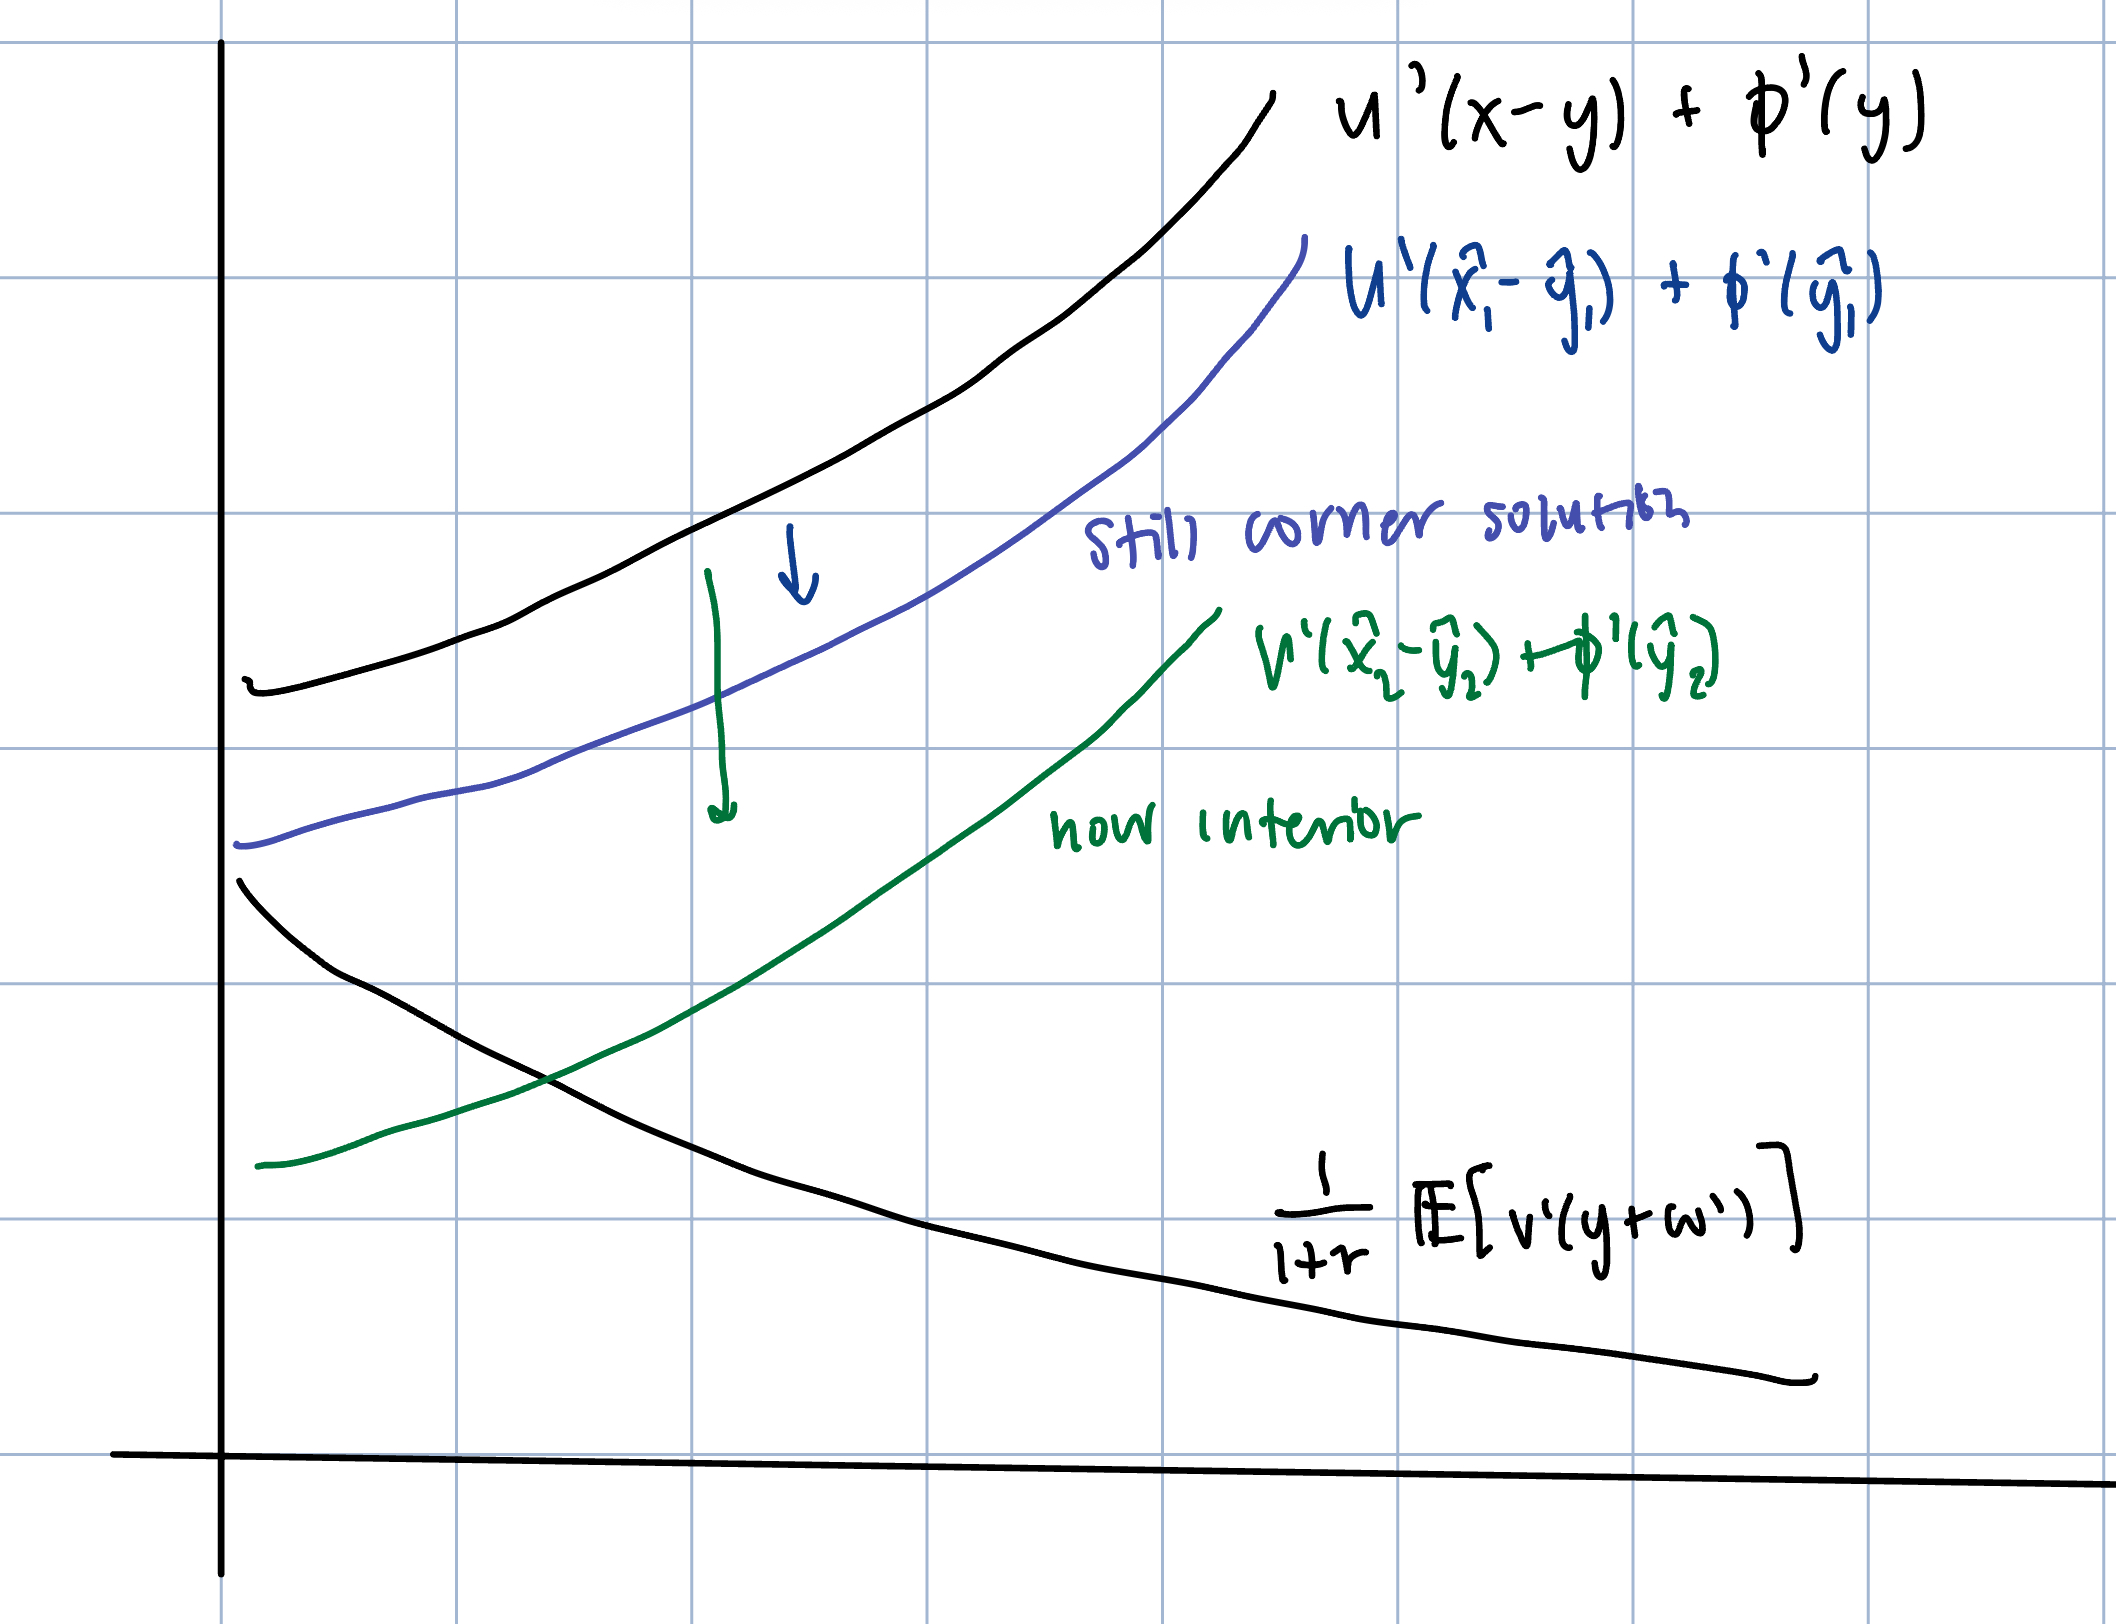
\includegraphics[width=0.5\textwidth]{11-6-3}
		\captionof{figure}{A corner solution can move to an interior solution or stay at the corner if $\hat{x} > x$.}
	\end{center}}Because the intersection moves down,
	\begin{align*}
		U'(\hat{x}-Y(\hat{x})) + \phi'(Y(\hat{x})) &< U'(x-Y(x)) +\phi'(Y(x)) \\
		\implies U'(\hat{x} - Y(\hat{x})) &< U'(x-Y(x))
	,\end{align*} since $\phi(Y(\hat{x})) > \phi'(Y(x))$. Then, \[
		\hat{x} - Y(\hat{x}) = c(\hat{x}) > c(x) = x-Y(x)
	,\] so consumption increases. 

	Notice that in the interior solution, consumption and storage increase. But in a corner solution, we may not increase everything; in this case, we just increase consumption (if storage stays at $0$) keeps the solution from moving interior.
\end{proof}

\subsection{Additional Properties of the Optimal Inventory Policy}
Note that the option to store goods may or may not be useful, depending on
\begin{enumerate}[(i)]
	\item Variation in endowment
	\item Cost of storage
	\item Discount rate
	\item Curvature in the utility function.
\end{enumerate}

We want to provide a sufficient condition for inventories to always be zero.
\begin{prop}
	If \marginnote{The LHS represents when storage would be most worthwhile to the planner.} 	\begin{equation}
		U'(M) + \phi'(0) \ge \frac{1}{1+r} \int_{m}^{M} U'(\omega')\mu(\omega')d\omega'  \label{11-6C1}
	,\end{equation}
	then storage is not valuable. In particular, if inventory begins at $0$, then no inventory is ever acquired.
\end{prop}

\begin{proof}
	Choose $\epsilon>0$ so (\ref{11-6C1}) holds with equality at $M+\epsilon$ on the RHS. We can verify that the value function of consuming all of the current endowment \[
		v(x) = U(x) + \frac{1}{1+r} \E\left[\frac{1}{r} U(\omega')\right] 
	\] with the state space $X = \left[ m,M+\epsilon \right]$ satisfies the Bellman equation with the optimal policy $Y(x) = 0$. The RHS implies that the current endowment $x$ is consumed entirely in the first period, and next period's endowment $\omega'$ is consumed entirely in next period. For a state space with a larger upper bound (so $x > M+\epsilon$ must be considered), it can be shown that there is an optimal decumulation policy.
\end{proof}

\begin{prop}
	A sufficient condition for storage to be sometimes worthwhile (and hence sometimes positive) is \begin{equation}  		U'(M) + \phi'(0) < \frac{1}{1+r} \int_{m}^{M} U'(\omega')\mu(\omega')d\omega' \label{11-11C2}
	.\end{equation}
\end{prop}

\begin{proof}
	The proof is similar, maybe.	
\end{proof}

\subsection{Long-run Properties of Inventories}

Together, the conditions (\ref{11-6C1}, \ref{11-11C2}) cover all cases.

\begin{prop}
	The exists a unique ergodic\marginnote{An ergodic set is the state space of a recursive and irreducible Markov chain.} set for $x$ and the distribution converges to it from any initial $x_0$.
\end{prop}

\begin{proof}
	Fix $X = \left[ m,\overline{x} \right]$, where $\overline{x} > M$. If (\ref{11-6C1}) holds, then inventories are depleted in finite time. So it remains to just show that the claim holds when (\ref{11-11C2})	holds. 

	Note that for any $x \in X$, there exists some $N \ge 1$ such that the stock hits zero with positive probability in $N $ periods. Thus the stock hits zero eventually with probability one. Note that irreduciblity in this case gives uniqueness. We need to show existence.

	There is a value $\hat{x} \in (m,\overline{x})$ with the property that \[
		Y(x) = 0, x \in [m,\hat{x}], \qquad x > \hat{x}
	.\] Furthermore, for $x > \hat{x}$, new inventories $Y(x)$ is strictly increasing with slope less than one.\marginnote{Slope less than one implies that if new supply is acquired, not all of it is carried over to next period; some is consumed in the current period.} We sketch the next period's beginning-of-period supply $x'$ as a function of current period's supply: \[
		x' = Y(x) + \omega'
	.\]
	\marginnote{
		\begin{center}
			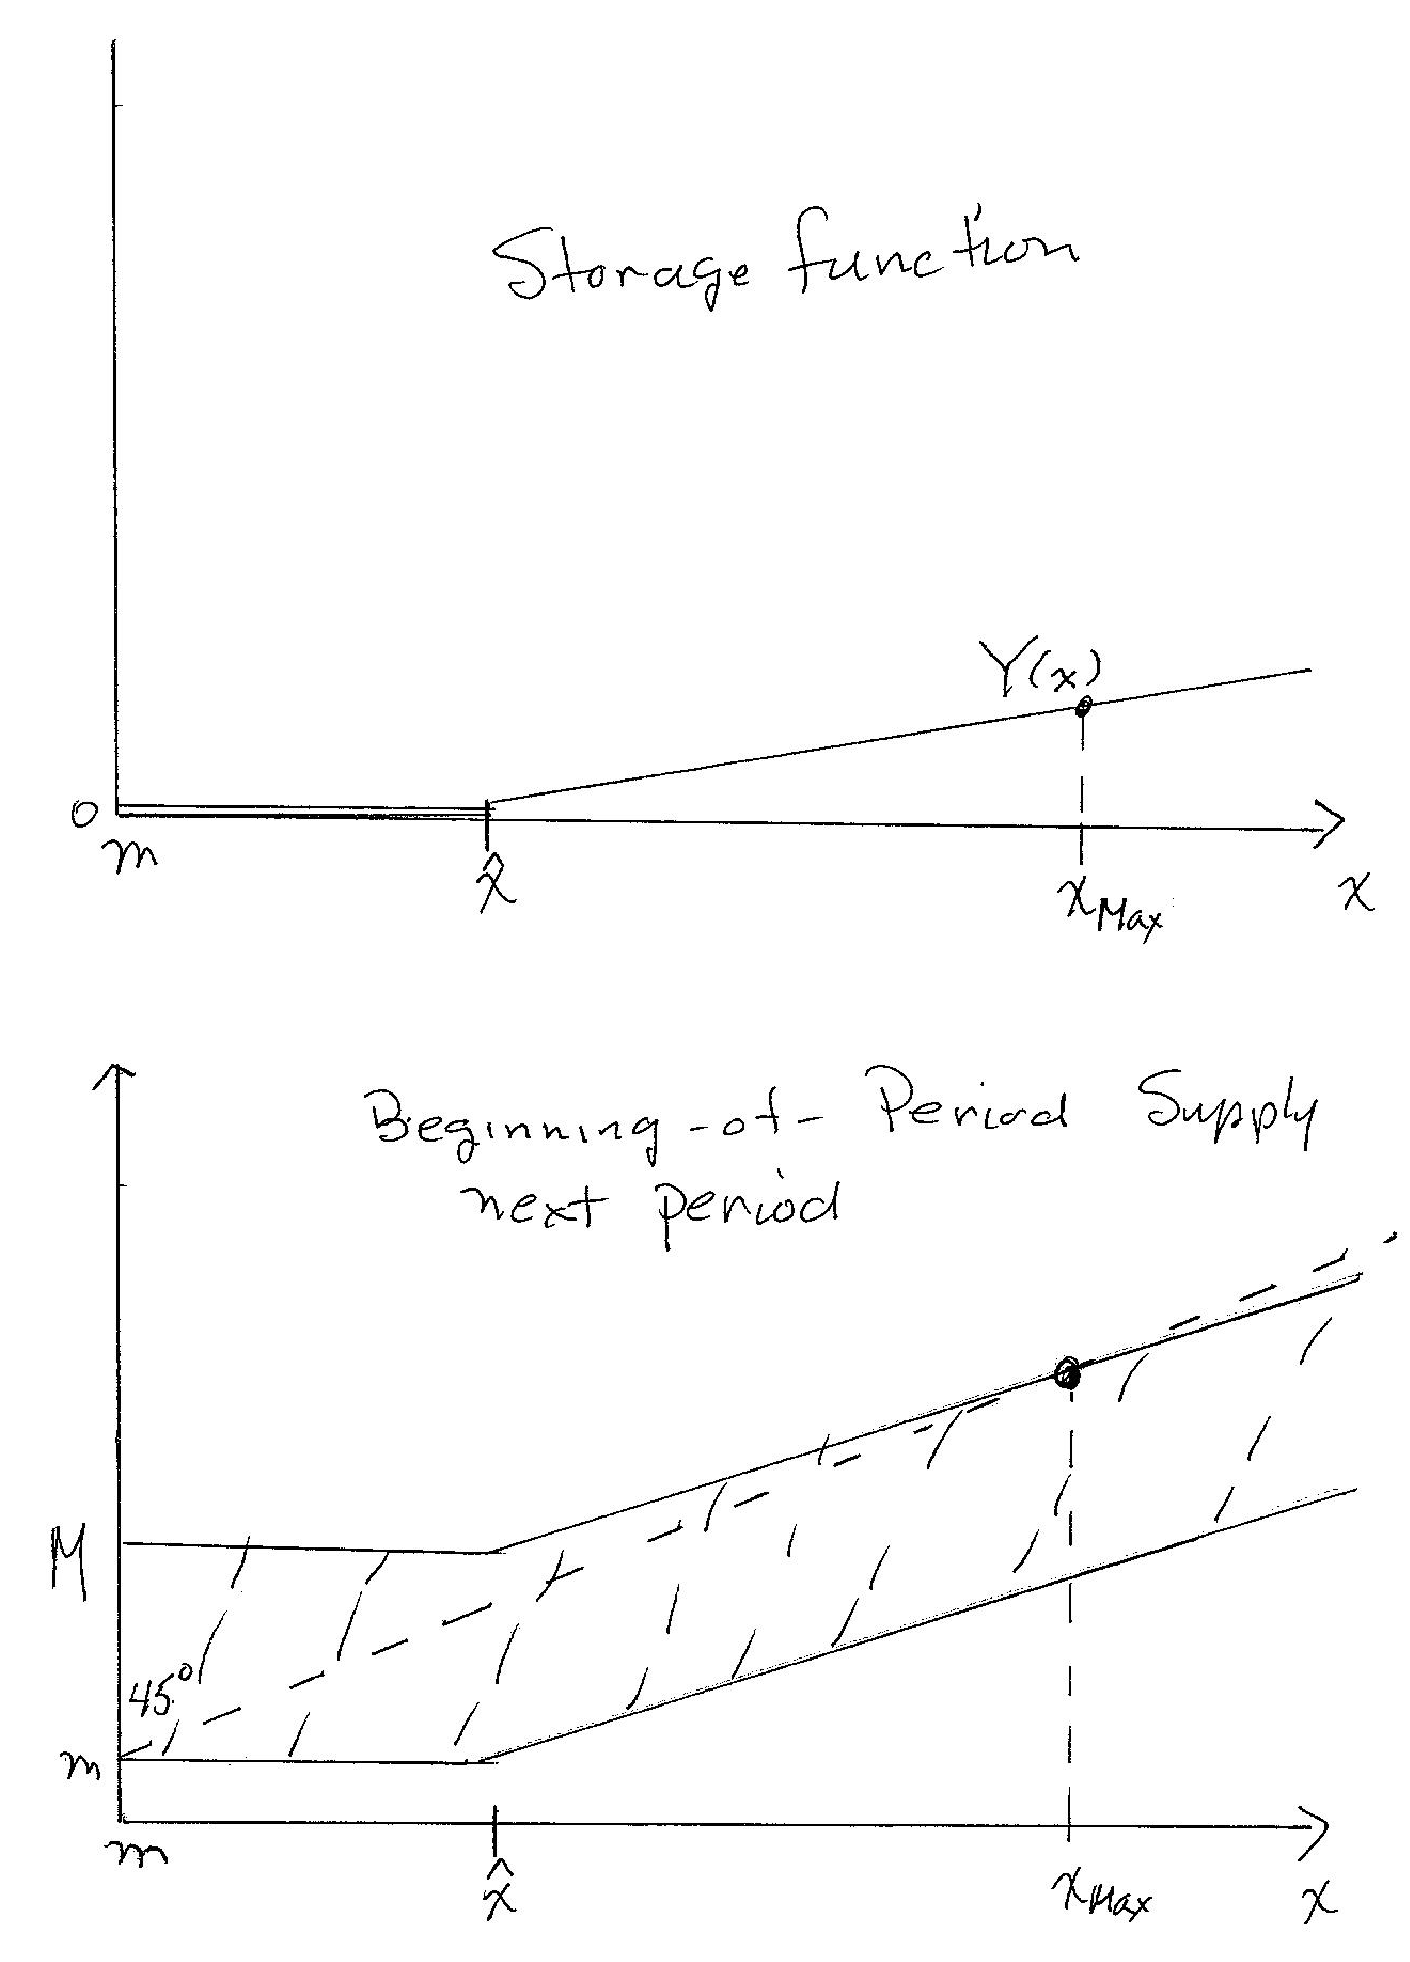
\includegraphics[width=0.5\textwidth]{11-11-1}
			\captionof{figure}{Storage function and future beginning-of-period supply}
		\end{center}
	}

	From an initial inventory of zero, the stochastic process going forward is always the same. So there exists a stationary distribution, and we know from before that it is unique. $\left[ m, x_{max} \right]$ is the ergodic set for beginning-of-period supply. \texthl{Review why we actually get existence.}

	For arguments relation to stationary distributions, we want to use the CDF. Note that since $x' = Y(x) + \omega'$, we get that for any $z \in \R$, \[
		x ' \le z \iff \omega' \le z- Y(x)
	.\] Define $\Psi(\omega) = \int_{m}^{\omega} \mu(\zeta)d\zeta $ as the CDF for the harvest. The conditional CDF for beginning-of-supply next period given current supply $x$ satisfies 
	\begin{align*}
		\P\left[x' \le z \mid x\right] &= \P\left[\omega' \le z- Y(x)\right]  \\
									   &= \Psi(z - Y(x))
	.\end{align*}

	The stationary CDF $G(\cdot )$ for beginning-of-period supply satisfies 
	\begin{equation}
		G(z) = \int_{m}^{\overline{x}} \Psi(z-Y(x))dG(x) , \quad z \in [m,\overline{x}] \label{eq:11-11G}
	.\end{equation}
	The LHS is the probability that $x' \le z$ next period, and the RHS is the integral of the conditional probabilities weighted by the stationary distribution itself.

	Now we consider prices. Recall that the price $p$ is a function of the state: \[
		p(x) = D(x-Y(x)) = U'(c(x))
	.\] Since $c$ is strictly increasing in $x$, the price is strictly decreasing in $x$. From (\ref{eq:11-11G}), we get the stationary CDF for price:
	\begin{align*}
		\P\left[p(x) \le b \right] &= \P\left[x \ge p^{-1}(b)\right]  \\
								  &= 1- G(p^{-1}(b))
	.\end{align*}

	Now we claim that if a storage technology is available, fluctuations in consumption and price are damped compared with what they are in an economy where storage is not possible. Claiming this concludes the proof.
\end{proof}

\subsection{Variable Inputs}
Some produces can respond to price fluctuations by adjusting variable inputs like land and labor.
Let $n$ be the quantity of inputs (an aggregate) used in production and $f(n,\omega')$ be the production function where it is strictly increasing, strictly concave in $n$, and satisfies \[
f(0,\omega') = 0, \qquad f'(0,\omega') = \infty
.\] 
Suppose these must be chosen in advance of the weather shock.
Assume inputs have a constant unit cost $c_0$. Then the Bellman equation is \[
 v\left(x \right) = \max_{n\ge 0, y\in[0,x]} U(x-y) - c_0 n - \phi(y) + \frac{1}{1+r} \int_{m}^{M} v(y+ f(n,\omega'))\mu(\omega')d\omega' 
.\] 

The behavior of the economy is similar to the one with an exogenous endowment, but there is further dampening on consumption and price swings, as depleted inventory can be built by increasing inputs and vice versa.

\section{Asset Pricing}

\subsection{Background}

We want to provide a general equilibrium framework for thinking about Fama's ``efficient markets'' hypothesis. We will characterize asset prices and how they depend on 
\begin{enumerate}[(i)]
	\item preferences (risk aversion, time preferences),
	\item current endowment, and
	\item properties of the stochastic process for relevant shocks.
\end{enumerate}

Lucas's model has the following characteristics:
\begin{itemize}
	\item General equilibrium model.
	\item One consumption good that is the numeraire for asset prices.
	\item A representatieve consumer has everyone's common preferences.
	\item Explicit production is not needed; it uses an endowment economy where the ``Lucas tree'' is a productive asset and can be traded for consumption goods.
	\item Endowments are stochastic.
\end{itemize}

Output is an exogenous first-order Markov process and in equilibrium, consumption equals endowment --- the only way to save is by buying trees. Hece, quantities consumed are exogenous and prices are endogenous.\marginnote{While nobody is trading trees for consumption goods in equilibrium, we are interested in the prices that lead to this result.}

To characterize prices, we use a recursive competitive equilibrium: we look at the consumption and portfolio decisions of the representative consumer, imposing market clearing, and then back out the prices.

\begin{rmk}
	We have a few more questions, collectively known as ``asset pricing puzzles.'' Among these are
	\begin{itemize}
		\item The equity premium puzzle: Average returns to equity are very high compared to returns on save assets (Mehra and Prescott, 1985).
		\item Excess voltality puzzle: Equity prices are volatile relative to dividends (Schiller).
		\item Risk-free rate puzzle: The risk-free rate is very low.
		\item No Trade Theorem (Milgrom and Stokey).
		\item More from Kocherlakota (1996) and others.
	\end{itemize}
\end{rmk}

\subsection{Environment and Markets Overview}

We now specialize to the Lucas tree asset–pricing environment.

There is a large number of consumers with identical preferences and identical asset endowments, so we can work with a representative consumer (RC). There is a single consumption good, which is \emph{not} storable, and serves as the numeraire in which asset prices are quoted.

There is no production sector. Instead, there is a finite set of assets, interpreted as “trees.” Each unit of asset $n$ is in fixed aggregate supply and yields a stream of the consumption good (its dividend) each period. A share in asset $n$ is a claim on that entire dividend stream. We normalize per capita supply of each asset to one, so holding the vector $1 = (1,\ldots,1)'$ corresponds to holding the per–capita “market portfolio” of trees.

Uncertainty is summarized by an \emph{aggregate} shock. The shock follows a first–order Markov process and determines both current dividends and the transition probabilities for future shocks. Dividends for different assets may be jointly first–order Markov, but the mapping from state to dividends need not be injective: two distinct aggregate states can imply the same current dividend vector while implying different transition probabilities for the future. There are no idiosyncratic shocks in this baseline model.\marginnote{With heterogeneous agents and/or incomplete markets, the cross–sectional distribution of asset holdings would also enter the state and destroy the simple RC structure.}

Asset shares are traded each period for the current consumption good, after that period’s dividends are realized and paid. Prices and allocations are time–invariant functions of the current aggregate state. The aggregate state variable is the current shock; the individual state variable for the RC is her portfolio vector of asset holdings.

In equilibrium quantities are trivial: each consumer optimally holds one unit of each asset and consumes the aggregate dividend per capita. The interesting object is the price system that supports this “no–trade” allocation. Our strategy is:
\begin{enumerate}[(i)]
	\item Fix an asset price function and solve the RC’s consumption–portfolio problem.
	\item Impose representativeness (market clearing): in every state the RC optimally chooses to keep holding $1$ and consume her dividend. This pins down the recursive competitive equilibrium (RCE) price matrix.
\end{enumerate}

\subsection{The Model}

Now we define the model primitives.

\newthought{Preferences}: The representative consumer has time–separable expected utility over consumption,
\[
	\E\left[ \sum_{t=0}^{\infty} \beta^t U(c_t) \right],
\]
where $U:\R_+ \to \R$ is twice continuously differentiable, strictly increasing, and strictly concave, and $\beta \in (0,1)$ is the discount factor.

\newthought{Shocks}: There is a finite set of aggregate states indexed by $j = 1,\ldots,J$. The state follows a first–order Markov process with transition matrix
\[
	Q = [q_{jk}]_{j,k=1}^J, \qquad q_{jk} = \P(j_{t+1} = k \mid j_t = j),
\]
so $q_{jk} \ge 0$ and $\sum_{k=1}^J q_{jk} = 1$ for each $j$. We assume $Q$ has a single ergodic set and no transient states; cycles are allowed (e.g., to capture seasonality).

\newthought{Assets (technology)}: There are $N$ assets, indexed by $n = 1,\ldots,N$, and the per capita supply of each asset is one. Dividends are functions of the aggregate state. Collect them in the $J \times N$ \emph{dividend matrix}
\[
	Y = [y_{jn}]_{j=1,\ldots,J}^{n=1,\ldots,N}.
\]
In state $j$, the row
\[
	y_{j\cdot} = (y_{j1},\ldots,y_{jN})
\]
gives the dividend on each asset. For asset $n$, the column
\[
	y_{\cdot n} = (y_{1n},\ldots,y_{Jn})^T
\]
gives its dividend across states.

\newthought{Aggregate state and heterogeneity}: If consumers differed in tastes or initial portfolios, the \emph{distribution} of asset holdings across types would generally affect prices and would therefore be part of the aggregate state. With identical preferences and identical per–capita endowments, the aggregate state can be summarized by the current shock alone, which justifies the RC formulation.\footnote{This is the same “representative agent” logic as in the standard Lucas (1978) asset–pricing model.}

\newthought{Market structure}: Asset trade occurs each period after the realization and payment of current dividends. Prices depend only on the current aggregate state $j$. Let
\[
	P = [p_{jn}]_{j=1,\ldots,J}^{n=1,\ldots,N}
\]
denote the $J \times N$ price matrix, where $p_{jn}$ is the price (in units of the consumption good) of one unit of asset $n$ in state $j$. In the RCE we seek, $P$ is stationary: it is a time–invariant function of $j$, not of calendar time.

\subsection{The Consumer's Problem}

Let $\tilde{y}_t$ denote the shock and the consumer's asset holdings in period $t$ be represented by a column vector $z_T \in R_+^N$. His problem is to choose $\{c_t, z_{t+1}\}_{t=0}^{\infty}$ to maximize the expected discounted lifetime utility: \[
	v(z_0,y_0) = \max_{\{c_t,z_{t+1}\}} \E\left[ \sum\limits_{t=0}^{\infty} \beta^{t} U(c_t) \mid y_0\right] 
.\] 

Let the state variable be $(z,j)$, individual asset holdings and aggregate state.\footnote{The aggregate state $j$ deterines the current dividend $y_j$, asset prices $p_j$, and expectations about next period's shock, $Q_j$.} The feasible set for the consumer should be closed and bounded and contain $1$ in the interior. Let \[
	Z = \left[ 1-\epsilon,1+\epsilon \right]^{N}
	,\] and let the feasible set (given $z \in Z$ and $j$) be\marginnote{Note that since the market meets after the dividend is paid, $p_j$ is the \emph{post-dividend} price.} \[
	\Gamma(z,j) = \{x\in Z : c= (y_j z) - \left[ p_j (x-z) \right] \ge 0\}
.\] 

Given a matrix $P$, the Bellman equation is \[
	v^P(z,j) = \max_{x \in \Gamma(z,j)} \left[ U\left[ (y_j z) - p_j(x-z) \right] + \beta \sum\limits_{k=1}^{J} q_{jk}v^P(x,k) \right]
.\] 

\newthought{Now we solve the consumer's problem.} The RHS of the Bellman equation is a contraction, so for any $P$, there is a unique fixed point $v^P$. For each $j$, $v^P(\cdot ,j)$ is weakly increasing in $z$, and strictly increasing if $P \gg 0$.\marginnote{$v^P$ is weakly increasing in $z$ if $y_{jn} + p_{jn} = 0$ for some $j,n$; this occurs if the transition matrix $Q$ has multiple ergodic sets or transient states -- and some assets have dividents that are strictly positive in only some ergodic sets or only in the transient set.}

We need to assume that $Q$ has only one ergodic set and no transient states, but allow cycles. From this assumption, we get that the limit of $Q^t$ has all rows identical. For some $T > 1$ (larger than the length of the cycle), \[
	\frac{1}{T} \sum\limits_{t=1}^{T}  Q^t \gg 0
.\] 

Note that for each $j$, $v^P(\cdot ,j)$ is strictly increasing and weakly concave in $z$. To see why concavity is weak, if two assets have dividends that are linearly dependent, the value function has ``flat'' segments and the optimal portfolio is not unique. However, consumption is still uniquely determined.

\begin{prop}
	Fix $P$ and let $v^P, G^P$ be the value function and policy correspondence. Fix $(\hat{z},j)$, and suppose there eis at least one optimal portfolio $x^*$ in the interior of $\Gamma(\hat{z}, j)$: \[
		x^* \in G^P(\hat{z},j), \qquad x^* \in \Gamma(\hat{z},j)^{\circ}
	.\] Then $v^P(\cdot ,j)$ is differentiable in $z$ at $\hat{z}$, and \[
		v_n^P(\hat{z},j) = \left. \frac{\partial v^P(z,j)}{\partial z_n} \right|_{z = \hat{z}} = U'\left[ (y_j\hat{z}) - p_j \left( x^* - \hat{z} \right) \right]\left( y_{jn} + p_{jn} \right)
	.\] 
\end{prop}

\subsection{Recursive Competitive Equilibrium}
\begin{defn}[Recursive Competitive Equilibrium]
	A Recursive Competitive Equilibrium is
	\begin{enumerate}[(i)]
		\item a price matrix $P^e = \left[ p_{jn}^{e} \right]$,
		\item value function, and policy correpondence \[
			v^e(z,j), \quad G^e(z,j), \quad z \in Z, j = 1,2,\ldots,J
		\] such that
	\end{enumerate}
	\begin{enumerate}[(i)]
		\item $v^e$ satisfies the household's Bellman Equation given $P^e$, and $G^e$ is the associated optimal policy correspondence, and
		\item we have representativeness: for initial assets $z = 1$\marginnote{$1$ is a column vector in $R^J$}, the portfolio $x = 1$ is optimal: \[
			1 \in G^e(1,j)
		.\] 
	\end{enumerate}

\end{defn}

After some work from the Euler equations, we eventually get that $P^e$ satisfies \[
	U'(c_j^e) p_{jn}^{e} = \beta \sum\limits_{k=1}^{J} q_{jk} U'(c_k^{e}) \left( y_{kn + p_{kn}^{e}} \right)
\] for all $n,j$, where $c_j^{e} = y_j \cdot 1$ is equilibrium consumption in state $j$.

\begin{prop}
	There exists a unique RCE such that $P^e \gg 0$.
\end{prop}
\begin{proof}
	Define
	\[
		a_j \equiv U'(c_j^e), \qquad j=1,\ldots,J,
	\]
	and let $A$ be the $J\times J$ diagonal matrix with diagonal
	$a = (a_1,\ldots,a_J)$, i.e.\ $A = \mathrm{diag}(a_1,\ldots,a_J)$.
	Let $Y = [y_{jn}]$ be the matrix of dividends and recall that
	$Q = [q_{jk}]$ is the Markov transition matrix.

	For a fixed asset $n$, collect the prices and dividends in
	$J\times 1$ vectors
	\[
		p_n^e = (p_{1n}^e,\ldots,p_{Jn}^e)^T, \qquad
		y_n = (y_{1n},\ldots,y_{Jn})^T .
	\]
	The Euler equations can then be written in vector form as
	\[
		A p_n^e \;=\; \beta Q A (y_n + p_n^e), \qquad \forall n.
	\]
	Stacking these equations over $n=1,\ldots,N$ gives the matrix equation
	\begin{equation}
		A P^e = \beta Q A (Y + P^e). \label{11-13-1}
	\end{equation}

	Rearranging,
	\[
		(I - \beta Q) A P^e = \beta Q A Y.
	\]
	Since $A$ is diagonal with strictly positive entries (because $U'$ is
	strictly positive) it is invertible.  Also, $Q$ is a transition matrix and
	$0<\beta<1$, so the Neumann series
	\[
		(I - \beta Q)^{-1} = I + \beta Q + \beta^2 Q^2 + \cdots
	\]
	converges, which shows that $I - \beta Q$ is invertible.  Hence from
	(\ref{11-13-1}) we obtain the solution
	\[
		P^e
		= A^{-1} (I - \beta Q)^{-1} \beta Q A Y.
	\]

	\emph{Uniqueness:} If $\widetilde P$ is another solution to (\ref{11-13-1}), then
	\[
		(I - \beta Q) A (P^e - \widetilde P) = 0,
	\]
	and multiplying by $A^{-1}(I - \beta Q)^{-1}$ yields $P^e = \widetilde P$.
	Thus the RCE price matrix is unique.

	\emph{Positivity:} Note that
	\[
		(I - \beta Q)^{-1} \beta Q
		= \sum_{t=1}^{\infty} \beta^t Q^t.
	\]
	Because $Q$ has a single ergodic set, there exists $T>1$ such that
	\[
		\frac{1}{T} \sum_{t=0}^T Q^t \gg 0,
	\]
	so in particular $\sum_{t=1}^T Q^t \gg 0$, and therefore
	$\sum_{t=1}^{\infty} \beta^t Q^t \gg 0$.  The matrices $A$ and $A^{-1}$
	are diagonal with strictly positive entries, and the dividend matrix
	$Y$ satisfies $Y \gg 0$ (each tree pays a strictly positive dividend in
	every state).  Hence
	\[
		P^e
		= A^{-1} \Bigl( \sum_{t=1}^{\infty} \beta^t Q^t \Bigr) A Y \gg 0.
	\]

	Thus there exists a unique recursive competitive equilibrium with
	strictly positive equilibrium prices $P^e \gg 0$.
\end{proof}

\subsection{Equilibrium Prices}
A portfolio is an $N\times 1$ column vector $\Lambda= \left( \lambda_1,\ldots,\lambda_N \right)^{T}$. 
The $J\times 1$ column vector $Y\Lambda$ gives the vector of payoffs from the portfolio $\Lambda$ in the $J$ states.

\begin{prop}
	If there is a set of assets with linearly dependent payoffs, i.e., if there exists $\Lambda = (\lambda_1,\ldots,\lambda_n)^{T} \ne 0$ such that\marginnote{Note that some $\lambda_i$s must be negative.}\[
		Y\Lambda_0 = 0
	,\] then $P^e (\Lambda_0)$.
\end{prop}

Let $e_{.j}$ denote the $J\times 1$ column vector with $1$ in the $j$th position and $0$s elsewhere.\marginnote{$e_{.j}$ is the return on an asset that pays one unit when state $j$ occurs and nothing otherwise.}

\begin{defn}[Spanning]
	The asset returns $Y$ span the state space if for each state $j$ there exists a column vector $\Lambda_{.j} = \left( \lambda_{1j},\ldots,\lambda_{Nj} \right)^{T}$ such that \[
		Y \Lambda_{.j} = e_{.j}
	\] for $j = 1,\ldots,J$.
\end{defn}
The portfolio $\Lambda_{.j}$ delivers one unit of goods when state $j$ occurs and zero otherwise.

\begin{prop}
	The asset returns span the state space if and only if there exist $J$ assets whose returns are linearly independent.
\end{prop}
\begin{proof}
	This is a standard linear algebra result.
\end{proof}

\begin{prop}
	Suppose the asset returns span the state space with the set of portfolios $\Lambda_{_.j}, \ldots,\Lambda_{.J}$. The $J\times J$ matrix $\Pi^{e} = P^e \Lambda$ contains the prices of infinitely-lived state-contingent claims: $\pi_{ij}^{e}$ is the price in state $i$ of a portfolio that delivers one unit of goods every time state $j$ occurs and zero otherwise.
\end{prop}



\newthought{How do we price a new asset?} Suppose the assets $Y$ span the state space.\marginnote{If $Y$ does not span the state space, the new asset can be priced iff its payoffs are a linear combination of the payoffs of old assets.} Consider the price of a new asset with return vector \[
	\hat{y} = \left( \hat{y}_1,\ldots,\hat{y}_J \right)
\] and a small amount $\epsilon > 0$ per capita is introduced. Consumption in each state changes very little, so equilibrium prices of old assets also change very little. The new asset can be priced as a linear combination of the assets $\left( \Lambda_{.1},\ldots,\Lambda_{.J} \right)$ with weights $\left( \hat{y}_1,\ldots,\hat{y}_J \right)$. 

Since the new asset delivers $\hat{y}_j$ when state $j$ occurs, the price vector is the $J\times 1$ column vector \[
	\hat{p} = \Pi^{e} \hat{y}
.\] 

After doing some manipulation, we can get that the equilibrium asset prices are \[
	P^e = A^{-1}\left[ \beta Q + \beta^2Q^2 + \beta^3Q^3+\ldots \right]AY
,\] where $A$ is a diagonal matrix with the marginal utility of consumption $a_j = u'(c_j)$ on the diagonal. 

\begin{ex}
	Suppose there is a large number of assets with i.i.d.\ dividends across assets and over time.
	We model this with by the following:
	Let $N$ be large and each asset's payoff take $K$ distinct values, so $J = K^{N}$ is very large. 
	Then consumption and marginal utility of consumption are approximately constant: \[
		c_j^e = y_j \cdot 1 \approx \overline{c}^{e}, \quad a_j = U'(y_j \cdot 1) \approx \overline{a}^e
	.\] Since consumption is approximately constant and all assets look the same going forward, asset prices are constant across assets and across states (over time).
\end{ex}

\begin{ex}
	(Serial correlation in an asset's dividend process) Suppose there are many assets with independent and symmetric dividend processes, but dividends are serially correlated for each asset. Then consumption is approximately constant, but the price of an asset varies with its current divided. Since the shocks are independent across assets, the cross-sectional distribution of asset prices is constant over time.

	Recall the price of asset $n$ in state $j$ is \[
		a_j p_{jn}^{e} = \beta \sum\limits_{k=1}^{J} q_{jk}a_k (y_{kn} + p_{kn}^{e}), \quad \forall n,j
	.\] 
	In this example, $a_j$ is approximately constant, so \[
		p_{jn}^{e} = \beta \sum\limits_{k=1}^{J} q_{jk} \left( q_{kn} + p_{kn}^{e} \right), \quad \forall n,j
	.\] 
\end{ex}

\begin{ex}
	(Insurance motive) Consider two states and two assets, so $J=N= 2$. Let \[
		Q = \begin{pmatrix}
		0.9 & 0.1 \\
		0.5 & 0.5
		\end{pmatrix} 
	\] and \[
		Y = \begin{pmatrix}
		10 & 0 \\
		0 & 1
	\end{pmatrix} 
	.\] Asset 2 is valuable since it provides a divided in bad times. Prices differ across states for two reasons: $q_{1\cdot } \ne q_{2\cdot }$ and $a_1 \ne a_2$. From the asset pricing equation, we see that \[
		\frac{a_k}{a_j} = \frac{U'(c_k^{e})}{U'(c_j^{e})}
	.\] The ratio of marginal utility of consumption is close to unity if the aggregate dividend doesn't vary much (where $c_j^{e} \approx c_k^{e}$) or if $U$ is close to linear, so $U'$ is almost constant.
\end{ex}

\subsection{Asset Pricing Equations Summary}
The price of asset $n$ in today's state $j$ is given by \[
	U'(c_j^e)p_{jn}^{e} = \beta \sum\limits_{k=1}^{J} q_{jk} U'(c_k^{e}) \left( y_{kn} + p_{kn}^{e} \right)
.\] The left hand side is the utility gain from selling the asset today then consuming, while the right hand side is the expected discounted utility of holding the asset until tomorrow, getting the dividend in whatever state $k$ is realized, then selling and consuming.

The price should be such that $c_j^e = y_j \cdot 1$.
We can represent all of these pricing equations with \[
	AP^{e} = \beta Q A(Y+P^{e})
.\] This yields \[
	p_{jn} = \frac{1}{U'(c_j^{e})} \left[ \beta Q + \beta^2 Q^2 + \ldots\right]_{j,\cdot} \begin{bmatrix}
		U'(c_1^{e}) Y_{n 1} \\
		\vdots \\
		U'(c_J^{e}) Y_{n J}
	\end{bmatrix} 
.\] Equivalently, we have \[
	P = A^{-1} (I - \beta Q)^{-1} \beta Q A Y
.\] 

\section{Aiyagari Model -- Savings with Idiosyncratic Income Shocks}

We wonder why in measurement, capital stock and investment are so high. Realistic wealth to income ratios are hard to generate in riskless models. Furthermore, the wealth distribution is even more skewed more than that of income. Furthermore, we hope to explain:
\begin{enumerate}[(i)]
	\item Individual income and consumptions are much more variable than the aggregates
	\item Individul and aggregate income and consumption are not very highly correlated\marginnote{Most risk is idiosyncratic and there isn't much risk sharing}
	\item Individual asset holdings are volatile.	
\end{enumerate}

We use an infinitely lived dynasty framework to examine self-insurance as a way to insure against idiosyncratic risk. In terms of individual behavior, we will answer:
\begin{enumerate}[(i)]
	\item How much more saving does an individual do?
	\item How effective is self-insurance in smoothing consumption?
\end{enumerate}
In the aggregate, we will answer:
\begin{enumerate}[(i)]
	\item What is the effect on aggregate saving, the aggregate capital stock, and the real interest rate?
\end{enumerate}

With complete insurance markets, individuals first insure against their idiosyncratic labor supply risk, so the consumption of each individual is constant over time.\marginnote{With complete markets, consumption levels can only differ across individuals if their initial conditions are different.} With incomplete markets, consumption depends on what assets are available to self-insure.

In Aiyagari (1994), physical capital is the only asset and there are no aggregate shocks. He examines the steady state, where capital stock, aggregate labor supply, and aggregate consumption are constant. Because of precuationary motives, individuals hold more assets than if shocks were absent.

As a preview of results:
\begin{itemize}
	\item Additional saving is very modest; it is about 3 percentage points
	\item Income and wealth distributions are positively skewed
	\item While the Gini coefficient rises, it is not big enough, and the wealth distribution is missing the upper tail.\marginnote{Entrepreneurial income or another big shock is needed to fit this tail.}
\end{itemize}

\subsection{The Model}
Consider a continuum of individiuals indexed on $[0,1]$ with idiosyncratic labor shocks. Let the individual labor supply $l \in L = \left[ \underline{l}, \overline{l} \right]$ be a first order Markov process with $\underline{l} > 0$. Let\marginnote{$G$ can be fit to data.} $G(l';l)$ be the transition function with continuous density $g(l';l)$ with the Feller property.\marginnote{With the Feller property, for any $l'$, $g(l';l)$ is continuous in $l$.} Let $\Phi(l)$ with density $\phi(l)$ be the unique invariant distribution, so \[
	\Phi(\hat{l}) = \int_{\underline{l}}^{\overline{l}}  G(\hat{l};l)\phi(l)dl, \qquad \forall\ \hat{l} \in L 
.\] Choose the units so average labor supply per capita is unity: \[
	\int_{\underline{l}}^{\overline{l}}  l \phi(l)dl = 1 
.\]

\newthought{Preferences} Let each agent have preferences \[
	U\left( c \right) = \E_0\left[\sum\limits_{t=0}^{\infty} \beta^{t} u(c_t)\right] 
\] with discount rate $\rho > 0 $ and \[
	\beta = \frac{1}{1+\rho} <1
\] is the discount factor. Assume $u$ is continuous, strictly increasing, strictly concave, and continuously differentiable with $u'(0) = \infty$.

\newthought{Technology} Suppose there are many identical competitive firms that rent capital and labor from households and produce output using the CRS technology \[
	Y = F(K,L)
,\] where $F$ is defined net of depreciation. Assume $F$ is continuous, strictly increasing, strictly quasiconcave, differentiable, and satisfies Inada conditions. Define $f(k) = F(k,1)$ so factor returns are \[
	r(k) = f'(k), \qquad w(k) = f(k) - kf'(k)
.\] 

We want to characterize the steady state, finding $k^{ss}$, $r^{ss} = f'(k^{ss})$, and $w^{ss} = f(k^{ss}) - k^{ss} f'(k^{ss})$.

\newthought{Our plan is as follows:} 
Fix factor prices $(w,r)$. The state variable for an individual is $(a,l)$, this current asset holdings are current labor supply shock. Let $G$ be the exogenous Markov process for $l$ and $\alpha^*(a,l;w,r)$ be the optimal policy function for the individual. Use these to define a transition function $P(a,l;w,r)$ on $S$. 
Then we can characterize the invariant joint distribution of $s=(a,l)$ under $P$, which is also the invariant distribution across individuals in the steady state. 

Summing across individuals, we can get the aggregate capital stock per capita $K^{av}$. We then check if factor returns are compatible with average assets: \[
	K^{av} \left[ w(k^{ss}), r(k^{ss}) \right] = k^{ss}
.\] If it's not, then we have to adjust $(w,r)$.

\subsection{The Consumer's Problem}

We can limit the wage rates and rental rate of capital to ones compatible with production function: pick a $\hat{k}$ and put \[
	r = f'(\hat{k}), \qquad w = f(\hat{k}) - \hat{k} f'(\hat{k})
.\] For notational simplicity, suppress $\hat{k}$. Fix $B \le 0$, an exogenously given lower bound on assets. The Bellman equation for the individual's consumption and saving decision is \[
	V(a,l) = \max_{a' \in \Gamma(a,l)} \left[ u\left[ (1+r)a + wl - a' \right] + \beta \int_{}^{} V(a',l')g(l';l)dl'  \right]
,\] where \[
	\Gamma(a,l) = \left[ B, (1+r)a + wl \right]
.\] 

We need restrictions on the assumptions.

\begin{enumerate}[(i)]
	\item We require the interest rate is less than the rate of time preference, so $r < \rho$. If $r=\rho$ and labor income $wl$ is constant, then any amount of wealth is optimal. If $wl$ is stochastic, then the agent acumulates infinite wealth.
	\item The interval $L$ of labor supply shocks and function $G$ must be so precautionary saving is worthwhile. When the agent has BOP assets of zero, he saves iff \[
		u'(wl) < \frac{1+r}{1+\rho} \int_{}^{} u'(wl') g(l';l)dl' 
	.\] Thus we have a joint restriction on the shock process $G$, marginal utility function $u'$, and the ratio $\frac{1+r}{1+\rho} < 1$.
	\item We need an upper bound $a^{\text{max}}$ so the state space is compact. We can achieve this with a restriction on $u$: assume $u$ has decreasing average risk aversion and ARA goes to zero as $c$ grows.\marginnote{The technical details are skipped.}
	\item The lower bound on assets should be determined for which the consumer remains solvent with probability 1; even when he has the lowest labor shock, his wage income is enough to pay the interest: \[
		B = -\frac{wl}{r}
	.\] \marginnote{Alternatively, we can take $B=0$ or $B > -\frac{wl}{r}$. Having $B < -\frac{wl}{r}$ is difficult but more commonly seen in instances of secured debt; e.g. when someone puts a house as collateral.}
\end{enumerate}

\subsection{Analysis of the Consumer's Problem}

Standard arguments show that $V$ is continuous, strictly increasing, and weakly concave in $a$ for each fixed $l$. To show strict concavity, note that the feasible set is convex and the objective function in the sequence problem strictly concave, so the problem has a unique optimal choice.

\marginnote{
	\begin{center}
		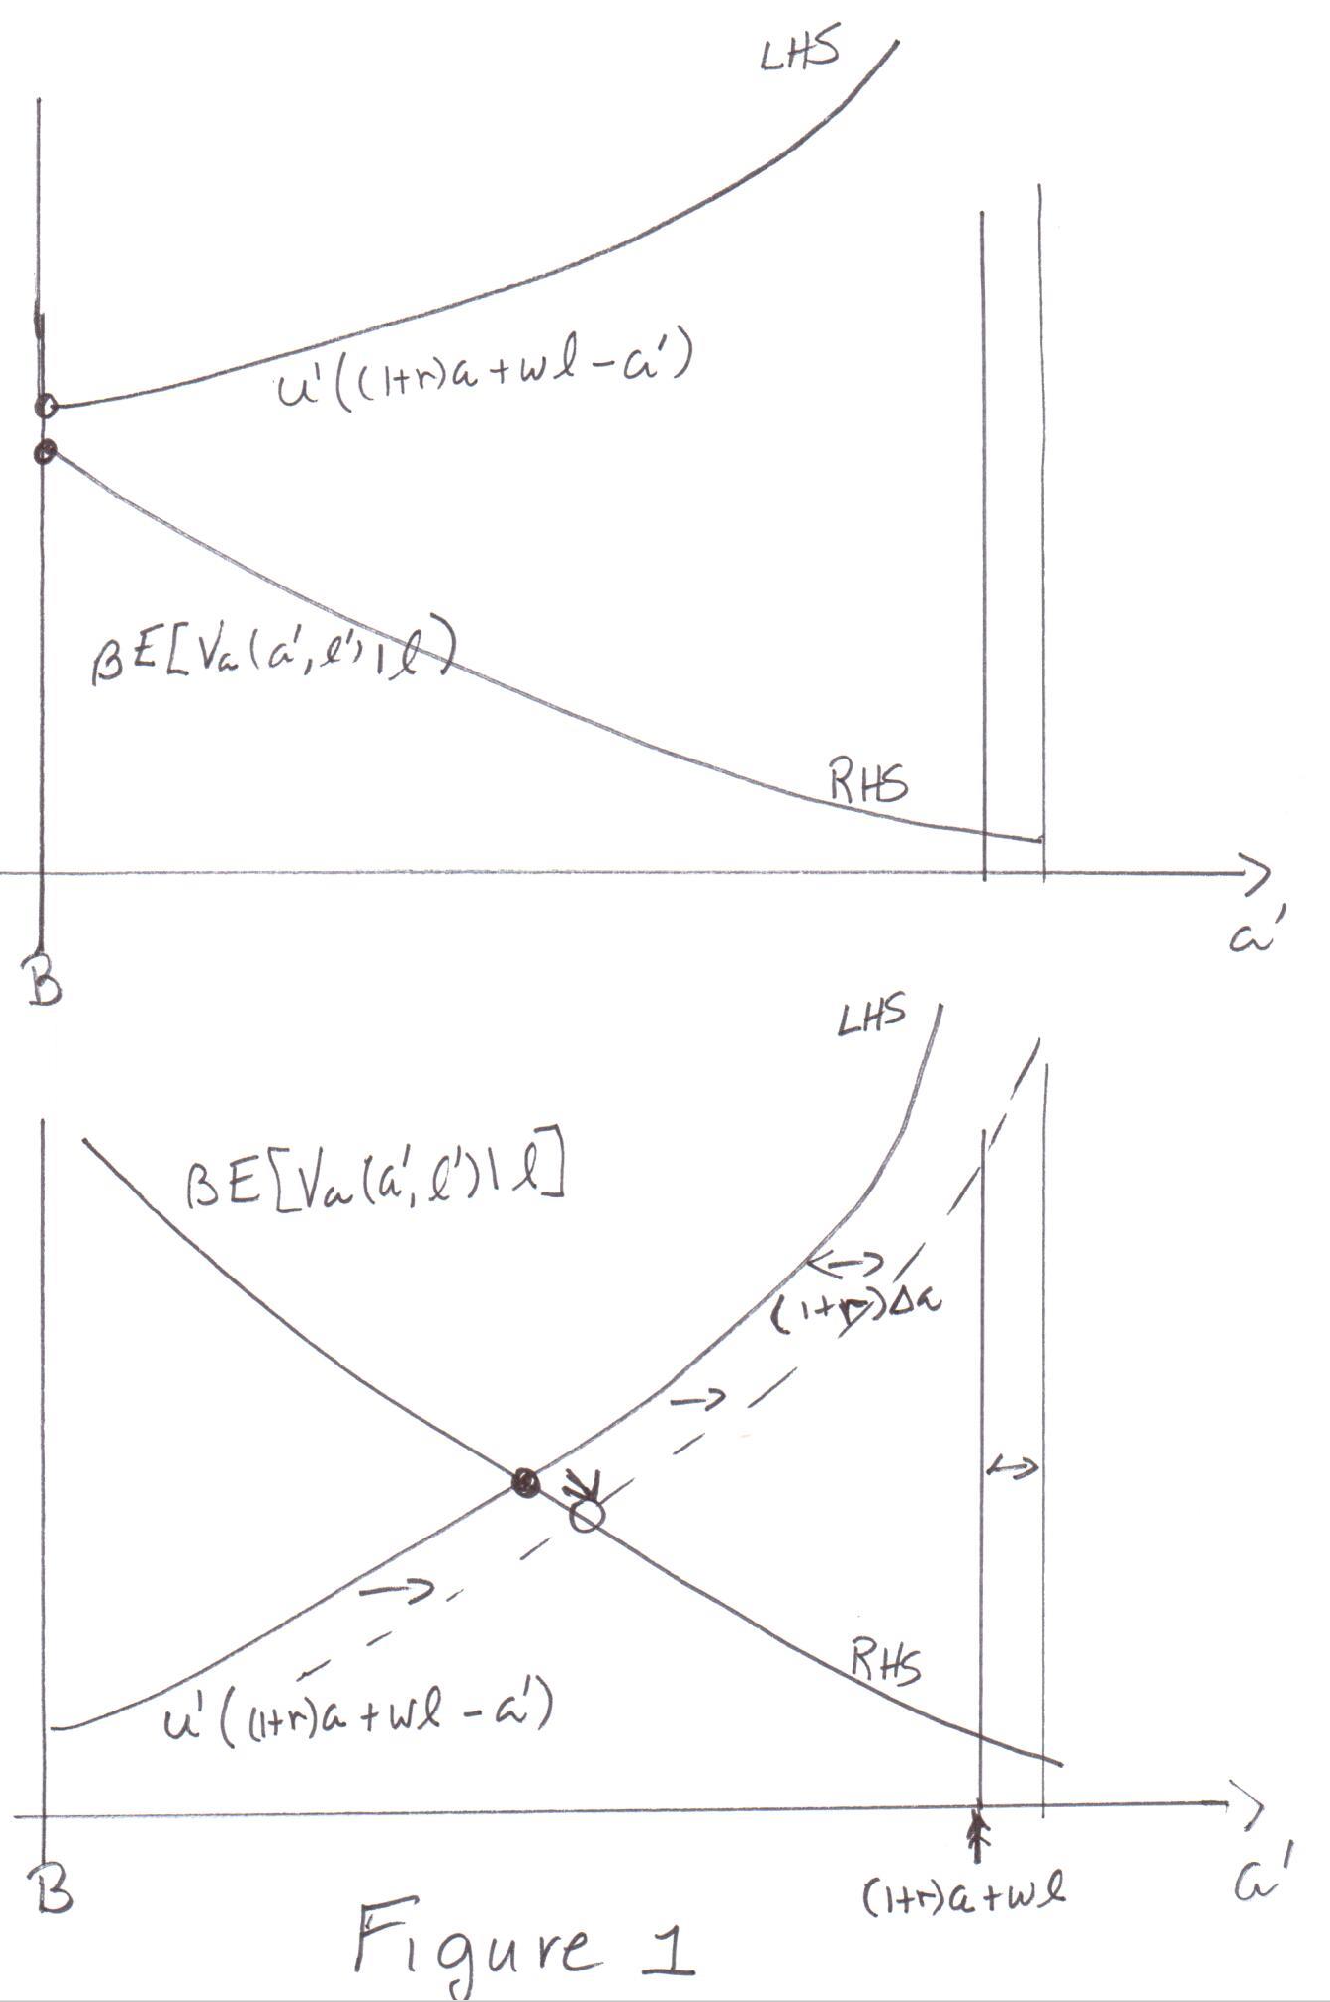
\includegraphics[width=0.5\textwidth]{11-20-1}
		\captionof{figure}{LHS and RHS of the FOC}
	\end{center}
}
The FOC is \[
	u'\left[ (1+r)a + wl - a' \right] \ge \frac{1}{1+\rho} \int_{}^{} V_a(a',l')dG(l';l) 
,\] with equality if $a' > B$. Referring to the plot, if $a$ increases by $\Delta$, the LHS is shifted to the right by $(1+r)\Delta$. As usual, if $a^* = B$, then the solution may either remain at $B$, or it may increase to be interior. If $a^* > B$, then $a^*$ increases by less than $(1+r)\Delta$, so consumption increases strictly.

The policy function $a^*$ has slope less than $(1+r)$, but the slope may exceed unity.

A higher labor shock in the current period has two effects:
\begin{itemize}
	\item It means a higher current income, providing an incentive to save more
	\item It improves earnings prospects for the near term, so the consumer is motivated to save less.
\end{itemize}

\subsection{The Transition Function for the State}
\marginnote{
	\begin{center}
		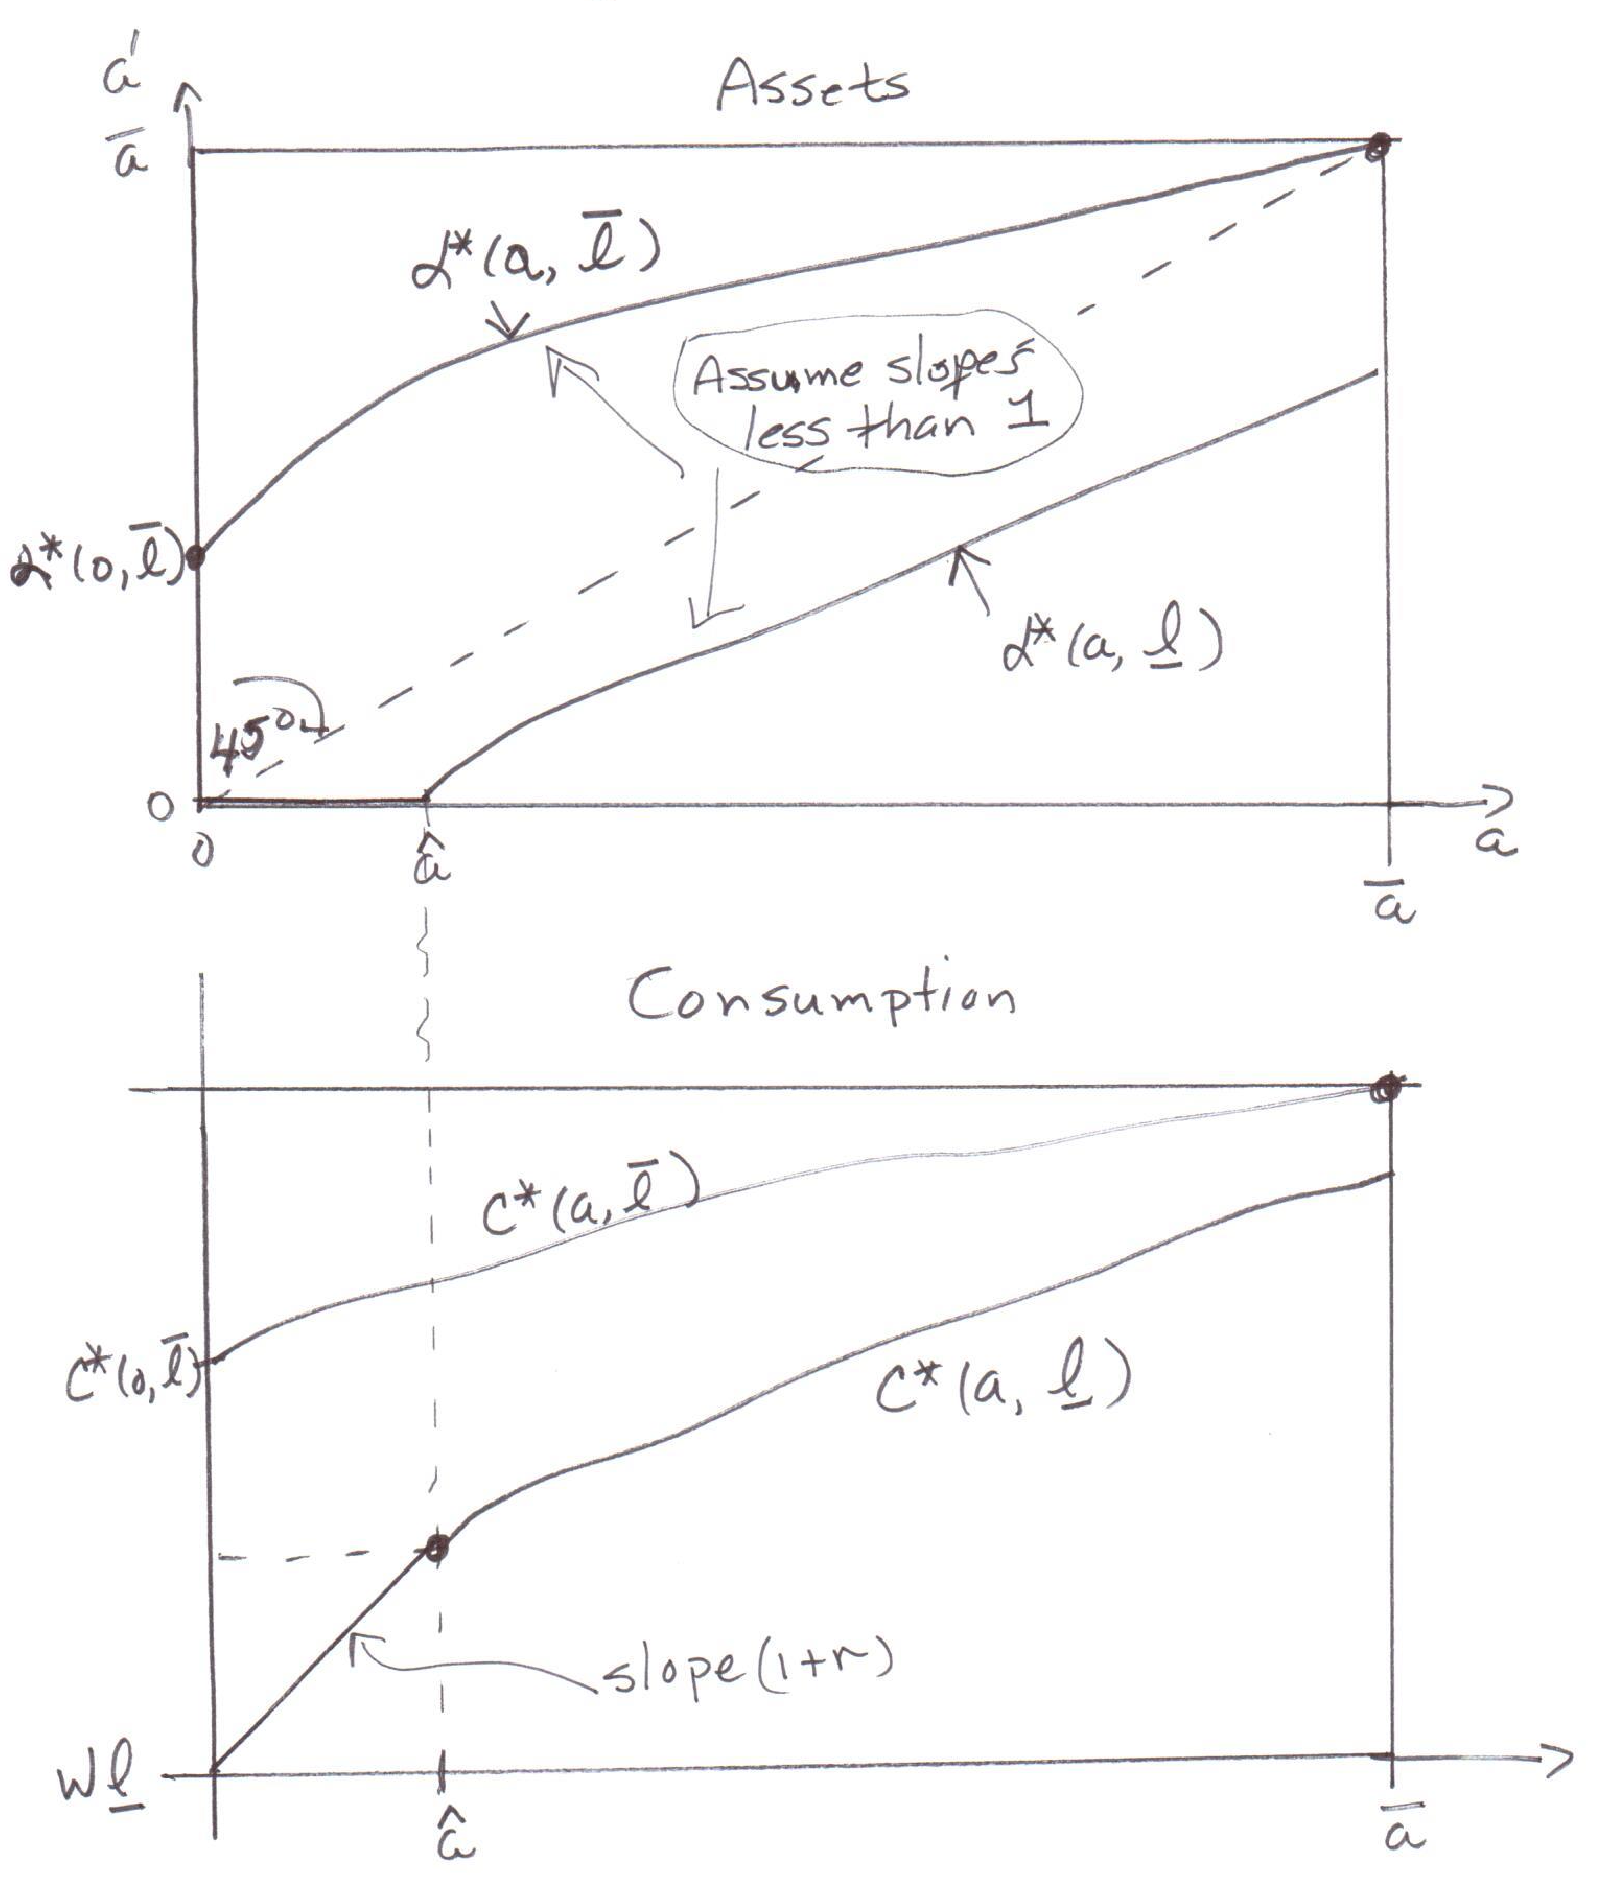
\includegraphics[width=0.5\textwidth]{11-20-2}
		\captionof{figure}{Policy functions with slope less than 1}
	\end{center}
}
If $a^*$ has slope less than 1, there is some interval of low labor shocks at which all income is consumed.

If $a^*$ has slope greater than 1, then there can be multiple ergodic sets and transient sets.
\begin{center}
	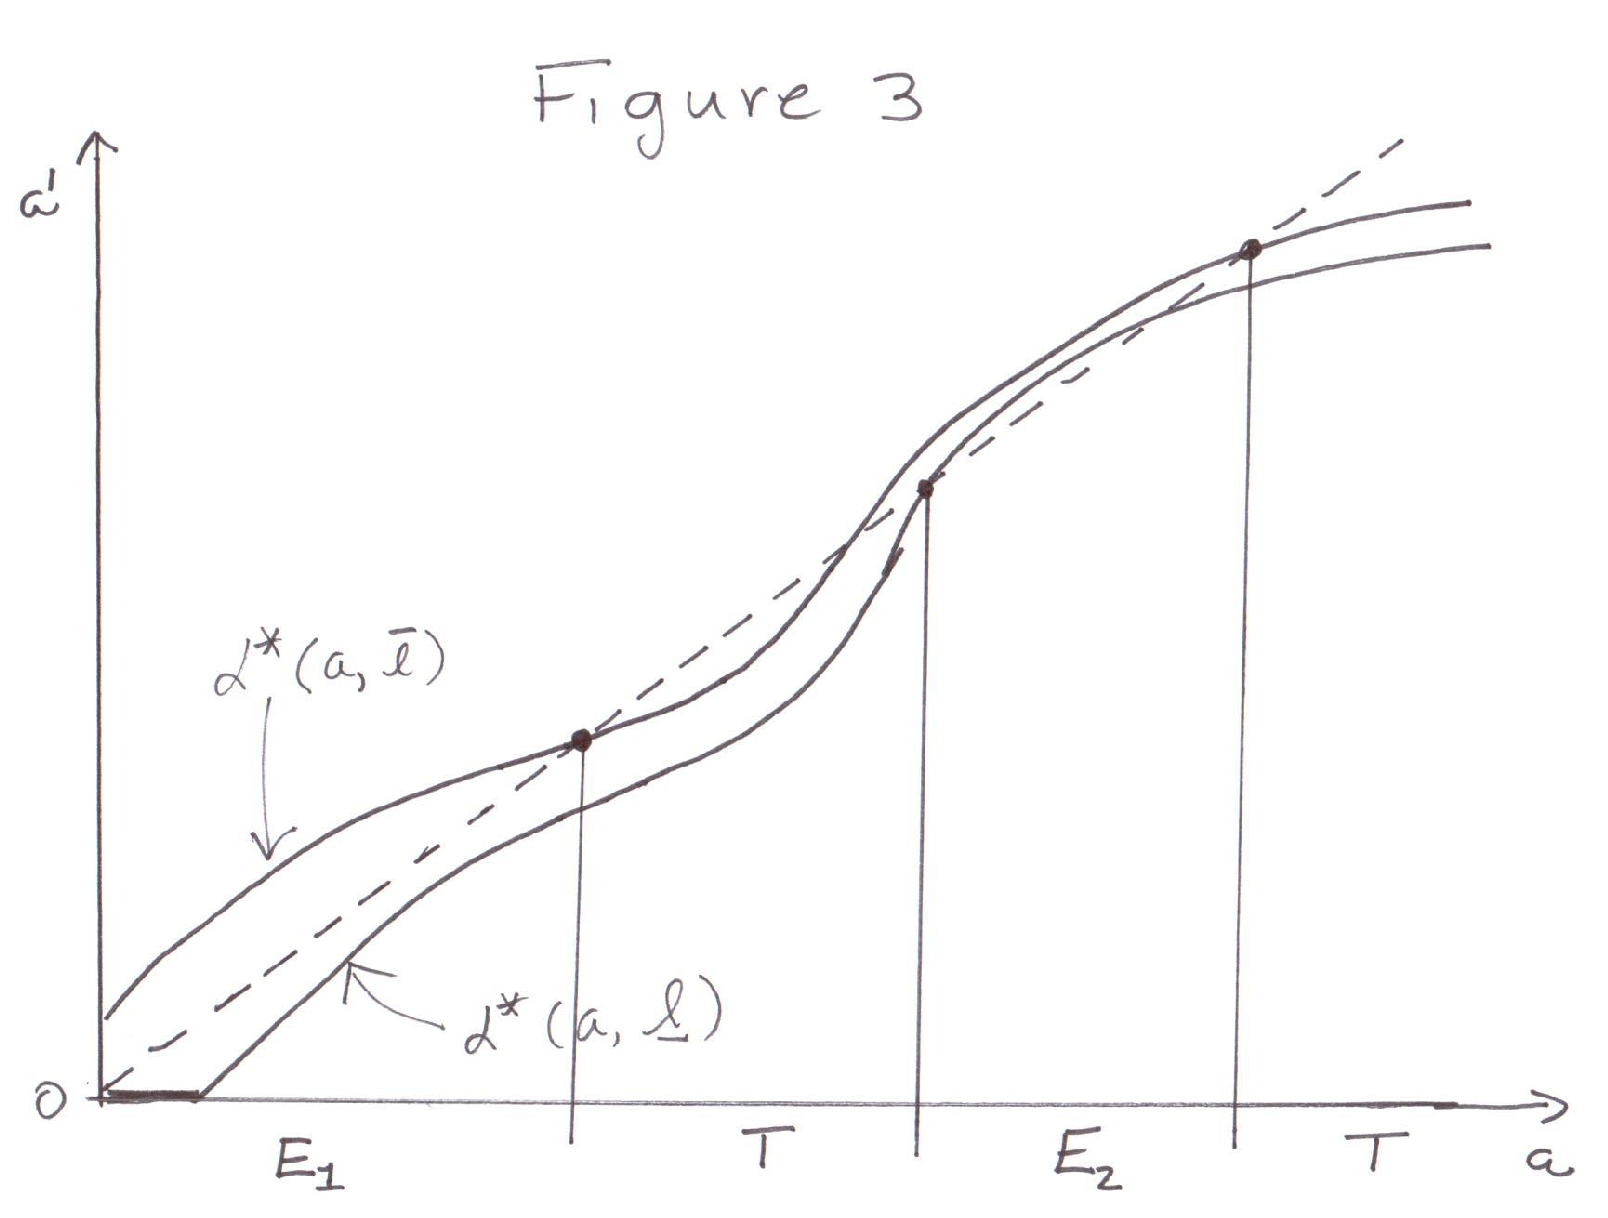
\includegraphics[width=0.5\textwidth]{11-20-3}
	\captionof{figure}{$a^*$ with slope greater than 1}
\end{center}
Note that if the individual is within sets $E_1$ or $E_2$, it is impossible for him to move to another set. Starting in a $T$ set leads the individual into $E_i$.

\subsection{The Stationary Distribution for i.i.d.\ Shocks}

The optimal policy function has the form \[
	a^*(a,l) = \sigma\left[ (1+r)a + wl \right]
,\] where $\sigma$ is nondecreasing and strictly increasing where $\sigma > 0$.

Hence, $a' \le z$ iff \[
	(1+r) a + wl \le \sigma^{-1}(z)
.\] The consumer carries over assets less than $z'$ if current-period goods-on-hand are low.\marginnote{We define $\sigma(0)$ as $\lim\limits_{z \to 0^+} \sigma^{-1}(z)$.}

\subsection{Average Assets and the Fixed Point Problem}
An increase in $\hat{k}$ change $r$ and $w$, and thus $K^{\text{av}}$. An increase in $\hat{k}$ has two effects:
\begin{itemize}
	\item price effect: $r$ decreases, so the price of insurance is higher, reducing the demand for insurance and thus reducing average assets
	\item income effect: a higher wage implies higher income, raising average assets.
\end{itemize}

The first effect dominates if there is a lot of risk or the consumer is very risk averse.

We plot the supply curve determined by its points $\left( K^{\text{av}}\left( r,w \right), r \right)$. 

\section{Search -- Lucas and Prescott Islands}
\subsection{Basic Search Model (McCall)}

Search models are a tractable model of market friction. In the McCall model, works decide to participate in the labor market or not; if they participate, if they are employed or not; if employed, if they quit and seek a new job.

At the beginning of each period, the worker can accept the wage $\hat{w}$ he was offered last period or reject it and continue searching. 
If he takes the job, he keeps it forever at the same wage. While unemployed, he may collected unemployment compensation. The goal is to maximize the EDV of total income.

Let $f$ be the density of the wage distribution, $b\ge 0$ unemployment benefits net of search bosts, $\beta = \frac{1}{1+r}$ the discount factor, and $\hat{w}$ the current wage offer. The state is $\hat{w}$, while the control is the binary choice of accepting or rejecting the current wage offer. Assume $F(b) < 1$ and $F(W) = 1$.

The Bellman equation is thus \[
	v(\hat{w}) = \max \{\underbrace{\frac{\hat{w}}{1-\beta}}_{\text{accept}}, \underbrace{b + \beta \int_{0}^{W} v(w)f(w)dw}_{\text{reject}} \}
.\] 
\marginnote{
	\begin{center}
		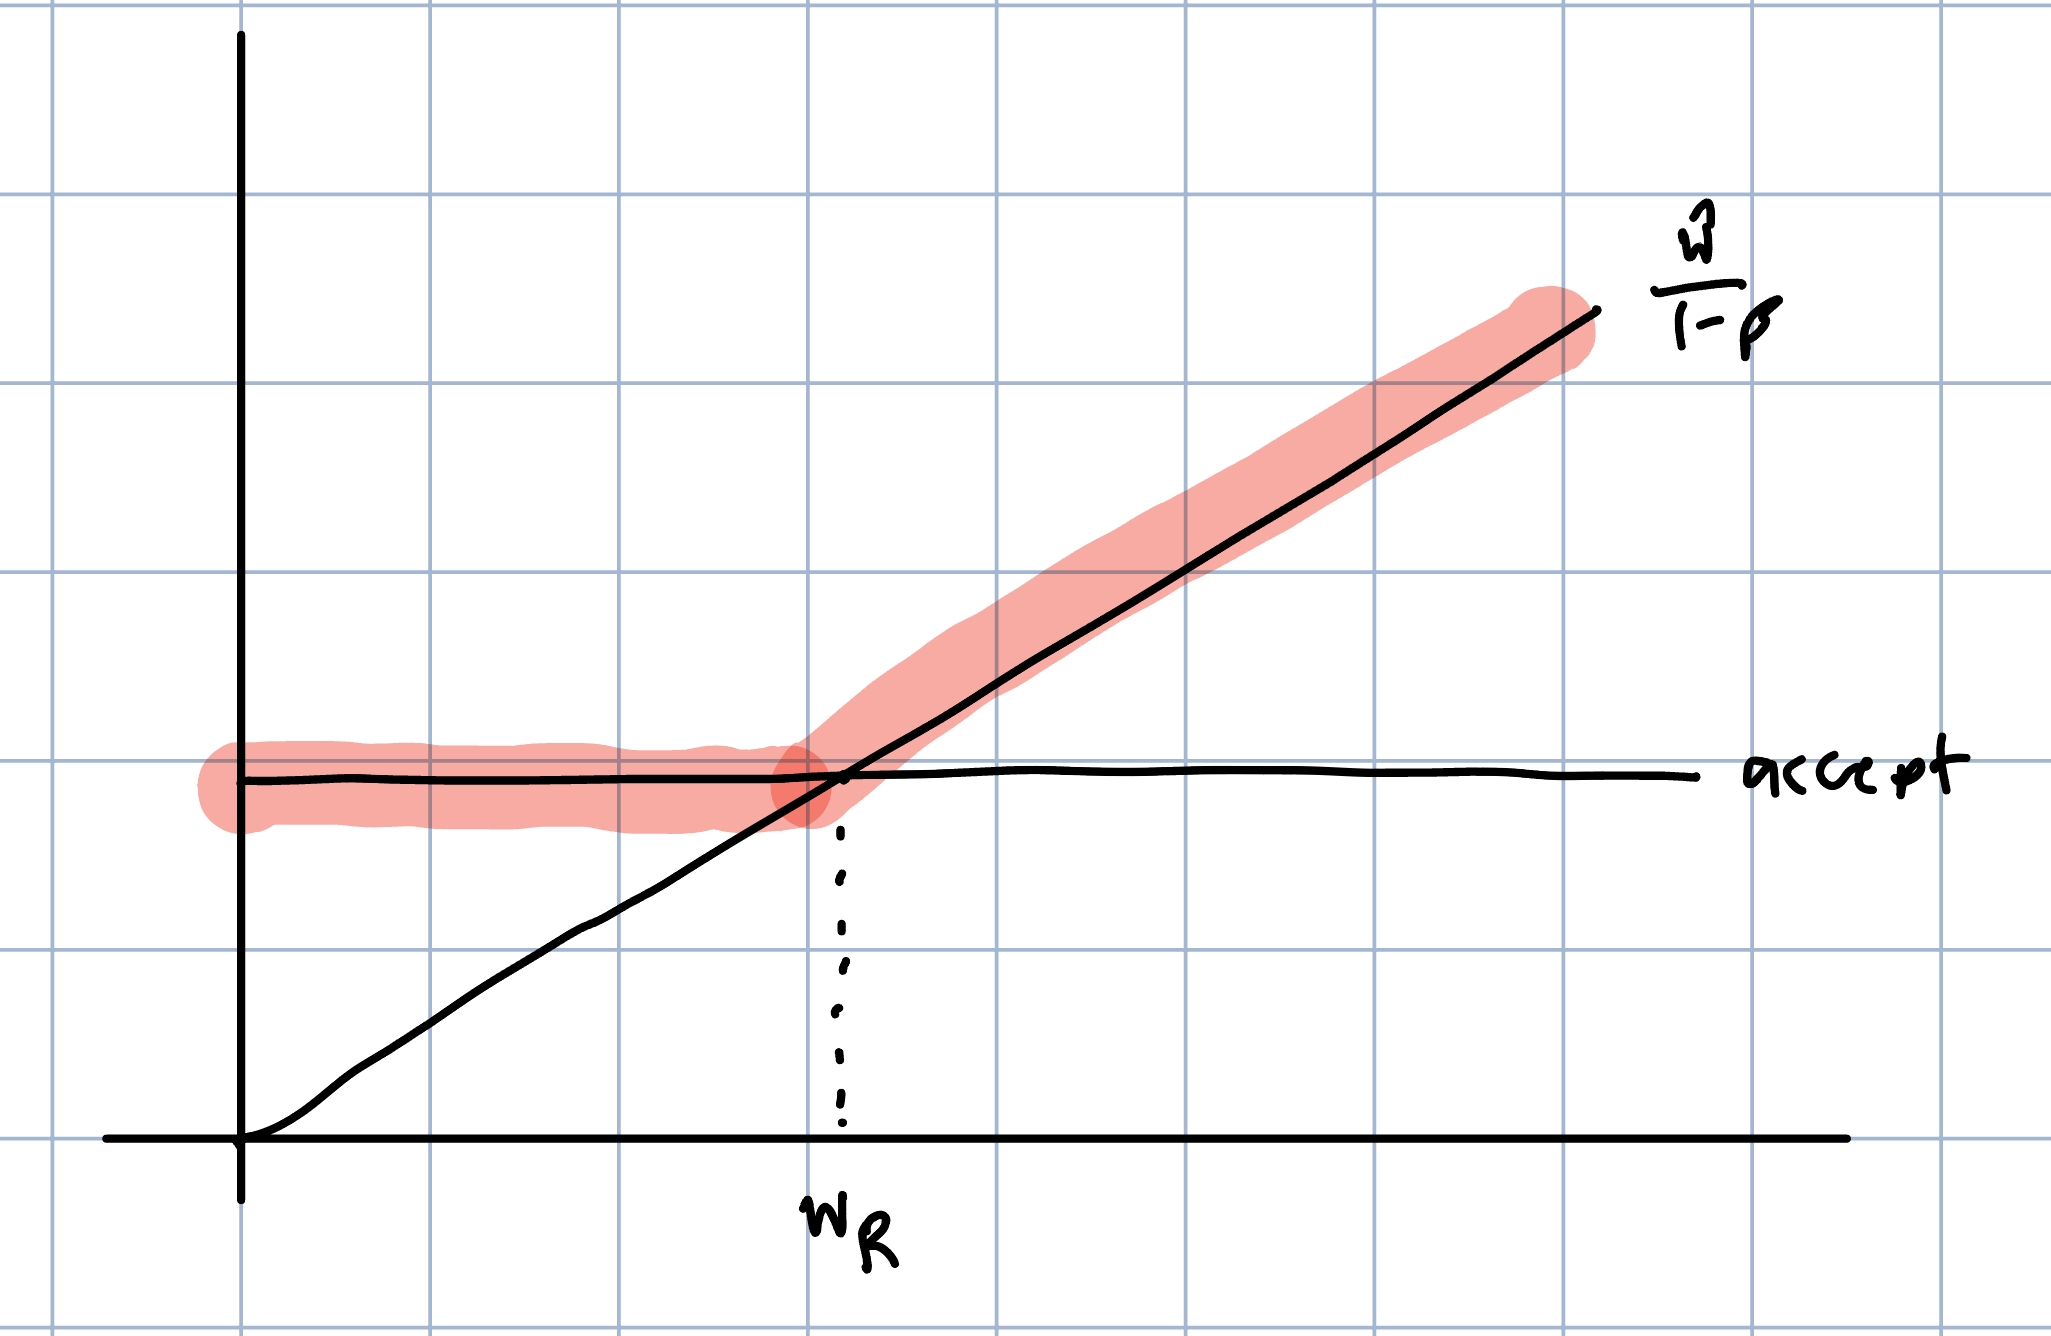
\includegraphics[width=0.5\textwidth]{12-2-1}
		\captionof{figure}{Bellman equation for McCall Search}
	\end{center}
}We see that $v$ is piecewise linear and there exists a reservation wage, where the decision to accept or reject depends only on how $\hat{w}$ relates to $w_R$.

To calculate $w_R$, we can put $\hat{w} = w_R$ in the Bellman to find the indifference point:
\begin{align*}
	v(w_R) = \frac{w_R}{1-\beta} &= b + \beta \left[ \frac{w_R}{1-\beta}F(w_R) + \int_{w_R}^{W} \frac{w}{1-\beta} f(w)dw  \right] \\
	w_R - b &= \frac{1}{r} \int_{w_R}^{W} (w-x)f(w)dw =: \frac{1}{r} \psi(w_R)
,\end{align*}
where $\psi(w_R)$ is the density-weighted surplus above $w_R$, appropriately discounted.

Note that $\psi(0) $ is the mean of the wage distribution, with $\psi(b) > 0$ and $\psi (W) = 0$. Furthermore, $\psi$ is decreasing, as $\psi'(x) = - \int_{x}^{W} f(w)dw < 0 $.
Plotting $x-b$ against $\frac{1}{r}\psi(x)$ as functions of $x$, the LHS of the equation for $w_R$ is strictly increasing (linear) from $0$ and the RHS is strictly decreasing starting from $\frac{\psi(b)}{r} > 0$ and is $0$ at $W$. So, there exists a unique intersection $w_R$.

As expected,
\begin{enumerate}[(i)]
	\item Less discounting $\implies w_R \uparrow$,
	\item $b \uparrow \implies w_R \uparrow$ ,
	\item An improvement in the wage distribution in the sense of FOSD raises $w_R$.
	\item Furthermore, a mean-preserving spread\marginnote{A mean preserving spread $G$ of $F$ means that for some $w^c$,
		\begin{align*}
			G(w) &\ge F(w), \forall\ w \le w^c, \\
			G(w) &\le F(w), \forall\ w \ge w^c
	.\end{align*}} raises the reservation wage. This is because draws from the left tail of the distribution are rejected anyways, so making them worse is inconsequential. Improving draws from the upper tail raises the reservation wage.
\end{enumerate}

The McCall model is problematic because it does not explain where unemployed workers come from. Furthermore, if firms are aware of how employment works, then they would just offer the reservation to everyone.

\subsection{Lucas-Prescott Islands: Overview}

Lucas-Prescott (1974) was the first to model unemployment for the entire economy.

They construct a model where workers sometimes choose to be unemployed, since a period of unemployment is the cost of searching for a new, higher-wage job. There are several islands that represent different labor markets\marginnote{The islands could be different occupations or geographical regions.} that are subject to idiosyncratic (yet identically distributed) productivity shocks. Hence, the cross-sectional distribution of shocks across islands is constant (in the long run), so each island operates in a stationary environment. The shocks follow a monotone Markov process.

Workers can move across islands with a cost, so they only move if the expected increase in value on the new island is sufficient large to compensate for foregone earnings.

Suppose an island has an increase in its productivity shocks. In the absence of labor inflows, the wage rate rises; due to the monotonicity of the Markov process, the expected value from next period also rises. This attracts new workers to the island. 
Workers flow across islands, and in equilibrium, the summed inflows equal the summed outflows.

We take a simpler (but equivalent) approach as the original paper. First, we study a representative island, and the rest-of-world is represented as another continent. The high-value continent is where exiting workers go, and the low-vlaue continent is the source of arriving new workers. The value gap between the two is such that workers on the low-value island are indifferent about migrating to the high-value island.

\subsection{Lucas-Prescott Islands: The Model}

\newthought{Preferences} Workers do not value leisure and their utility is linear in consumption. Their objective is to maximize \[
	\E\left[\sum\limits_{t=0}^{\infty} \beta^{t}c_t\right] 
.\] A worker on either continent can stay there forever with a constant wage.

\newthought{Labor supply} There are $N>0$ workers per island.

\newthought{Productivity shocks} The shock on an island is $z \in Z = \left[ \underline{z} , \overline{z} \right]$ with transition function $Q(z,z')$. Assume $Q$ has the Feller property, is monotone, satisfies a \emph{mixing condition}\marginnote{The mixing condition guarantees a unique ergodic solution. The fact that the same $n$ works for every $z$ implies that there are no cycles.} for some $n \ge 1, \alpha > 0$ \[
	Q^n(z,(a,b]) \ge \alpha(b-a) > 0, \quad \forall\ z\in Z, \forall\ \underline{z} \le z \le b \le \overline{z}
.\] Then $Q$ has a unique stationary distribution with stationary probability measure $\mu(z)$.

\newthought{Technology} Let $x$ be the beginning-of-period workforce and $z$ the shock. The wage $f(x,z)$ is marginal product, which is continuous and strictly decreasing in $x$ and strictly increasing in $z$ such that 
 $\forall\ z$, $f(0,z)$ is finite and $f(\overline{x}, z) = 0$.

\newthought{Timing} We have that $x$ is the beginning-of-period workforce on the island. Then this peirod's shock $z$ is realized. Workers on the island decide whether to stay or leave, workers form outside can arrive, and production and consumption occur.












\end{document}
